% Options for packages loaded elsewhere
\PassOptionsToPackage{unicode}{hyperref}
\PassOptionsToPackage{hyphens}{url}
%
\documentclass[
  ignorenonframetext,
]{beamer}
\usepackage{pgfpages}
\setbeamertemplate{caption}[numbered]
\setbeamertemplate{caption label separator}{: }
\setbeamercolor{caption name}{fg=normal text.fg}
\beamertemplatenavigationsymbolsempty
% Prevent slide breaks in the middle of a paragraph
\widowpenalties 1 10000
\raggedbottom
\setbeamertemplate{part page}{
  \centering
  \begin{beamercolorbox}[sep=16pt,center]{part title}
    \usebeamerfont{part title}\insertpart\par
  \end{beamercolorbox}
}
\setbeamertemplate{section page}{
  \centering
  \begin{beamercolorbox}[sep=12pt,center]{part title}
    \usebeamerfont{section title}\insertsection\par
  \end{beamercolorbox}
}
\setbeamertemplate{subsection page}{
  \centering
  \begin{beamercolorbox}[sep=8pt,center]{part title}
    \usebeamerfont{subsection title}\insertsubsection\par
  \end{beamercolorbox}
}
\AtBeginPart{
  \frame{\partpage}
}
\AtBeginSection{
  \ifbibliography
  \else
    \frame{\sectionpage}
  \fi
}
\AtBeginSubsection{
  \frame{\subsectionpage}
}

\usepackage{amsmath,amssymb}
\usepackage{iftex}
\ifPDFTeX
  \usepackage[T1]{fontenc}
  \usepackage[utf8]{inputenc}
  \usepackage{textcomp} % provide euro and other symbols
\else % if luatex or xetex
  \usepackage{unicode-math}
  \defaultfontfeatures{Scale=MatchLowercase}
  \defaultfontfeatures[\rmfamily]{Ligatures=TeX,Scale=1}
\fi
\usepackage{lmodern}
\ifPDFTeX\else  
    % xetex/luatex font selection
\fi
% Use upquote if available, for straight quotes in verbatim environments
\IfFileExists{upquote.sty}{\usepackage{upquote}}{}
\IfFileExists{microtype.sty}{% use microtype if available
  \usepackage[]{microtype}
  \UseMicrotypeSet[protrusion]{basicmath} % disable protrusion for tt fonts
}{}
\makeatletter
\@ifundefined{KOMAClassName}{% if non-KOMA class
  \IfFileExists{parskip.sty}{%
    \usepackage{parskip}
  }{% else
    \setlength{\parindent}{0pt}
    \setlength{\parskip}{6pt plus 2pt minus 1pt}}
}{% if KOMA class
  \KOMAoptions{parskip=half}}
\makeatother
\usepackage{xcolor}
\newif\ifbibliography
\setlength{\emergencystretch}{3em} % prevent overfull lines
\setcounter{secnumdepth}{-\maxdimen} % remove section numbering


\providecommand{\tightlist}{%
  \setlength{\itemsep}{0pt}\setlength{\parskip}{0pt}}\usepackage{longtable,booktabs,array}
\usepackage{calc} % for calculating minipage widths
\usepackage{caption}
% Make caption package work with longtable
\makeatletter
\def\fnum@table{\tablename~\thetable}
\makeatother
\usepackage{graphicx}
\makeatletter
\def\maxwidth{\ifdim\Gin@nat@width>\linewidth\linewidth\else\Gin@nat@width\fi}
\def\maxheight{\ifdim\Gin@nat@height>\textheight\textheight\else\Gin@nat@height\fi}
\makeatother
% Scale images if necessary, so that they will not overflow the page
% margins by default, and it is still possible to overwrite the defaults
% using explicit options in \includegraphics[width, height, ...]{}
\setkeys{Gin}{width=\maxwidth,height=\maxheight,keepaspectratio}
% Set default figure placement to htbp
\makeatletter
\def\fps@figure{htbp}
\makeatother

\makeatletter
\@ifpackageloaded{caption}{}{\usepackage{caption}}
\AtBeginDocument{%
\ifdefined\contentsname
  \renewcommand*\contentsname{Table of contents}
\else
  \newcommand\contentsname{Table of contents}
\fi
\ifdefined\listfigurename
  \renewcommand*\listfigurename{List of Figures}
\else
  \newcommand\listfigurename{List of Figures}
\fi
\ifdefined\listtablename
  \renewcommand*\listtablename{List of Tables}
\else
  \newcommand\listtablename{List of Tables}
\fi
\ifdefined\figurename
  \renewcommand*\figurename{Figure}
\else
  \newcommand\figurename{Figure}
\fi
\ifdefined\tablename
  \renewcommand*\tablename{Table}
\else
  \newcommand\tablename{Table}
\fi
}
\@ifpackageloaded{float}{}{\usepackage{float}}
\floatstyle{ruled}
\@ifundefined{c@chapter}{\newfloat{codelisting}{h}{lop}}{\newfloat{codelisting}{h}{lop}[chapter]}
\floatname{codelisting}{Listing}
\newcommand*\listoflistings{\listof{codelisting}{List of Listings}}
\makeatother
\makeatletter
\makeatother
\makeatletter
\@ifpackageloaded{caption}{}{\usepackage{caption}}
\@ifpackageloaded{subcaption}{}{\usepackage{subcaption}}
\makeatother

\ifLuaTeX
  \usepackage{selnolig}  % disable illegal ligatures
\fi
\usepackage{bookmark}

\IfFileExists{xurl.sty}{\usepackage{xurl}}{} % add URL line breaks if available
\urlstyle{same} % disable monospaced font for URLs
\hypersetup{
  pdftitle={Dealing with categorical variables},
  pdfauthor={Mohamed Ahmed Aref},
  hidelinks,
  pdfcreator={LaTeX via pandoc}}


\title{Dealing with categorical variables}
\author{Mohamed Ahmed Aref}
\date{}

\begin{document}
\frame{\titlepage}


\begin{frame}{Quarto}
\phantomsection\label{quarto}
Quarto enables you to weave together content and executable code into a
finished presentation. To learn more about Quarto presentations see
\url{https://quarto.org/docs/presentations/}.
\end{frame}

\begin{frame}{Bullets}
\phantomsection\label{bullets}
When you click the \textbf{Render} button a document will be generated
that includes:

\begin{itemize}
\tightlist
\item
  Content authored with markdown
\item
  Output from executable code
\end{itemize}
\end{frame}

\begin{frame}[fragile]{Code}
\phantomsection\label{code}
When you click the \textbf{Render} button a presentation will be
generated that includes both content and the output of embedded code.
You can embed code like this:

\begin{verbatim}
Rows: 21,483
Columns: 9
$ year    <int> 2000, 2000, 2000, 2000, 2000, 2000, 2000, 2000, 2000, 2000, 20~
$ marital <fct> Never married, Divorced, Widowed, Never married, Divorced, Mar~
$ age     <int> 26, 48, 67, 39, 25, 25, 36, 44, 44, 47, 53, 52, 52, 51, 52, 40~
$ race    <fct> White, White, White, White, White, White, White, White, White,~
$ rincome <fct> $8000 to 9999, $8000 to 9999, Not applicable, Not applicable, ~
$ partyid <fct> "Ind,near rep", "Not str republican", "Independent", "Ind,near~
$ relig   <fct> Protestant, Protestant, Protestant, Orthodox-christian, None, ~
$ denom   <fct> "Southern baptist", "Baptist-dk which", "No denomination", "No~
$ tvhours <int> 12, NA, 2, 4, 1, NA, 3, NA, 0, 3, 2, NA, 1, NA, 1, 7, NA, 3, 3~
\end{verbatim}

\begin{verbatim}
[1] White Black Other
Levels: Other Black White Not applicable
\end{verbatim}

\begin{verbatim}
[1] White Black Other
Levels: Other Black White Not applicable
\end{verbatim}

\begin{verbatim}
# A tibble: 3 x 2
  race      n
  <fct> <int>
1 White 16395
2 Black  3129
3 Other  1959
\end{verbatim}

\begin{verbatim}
# A tibble: 3 x 2
  race      n
  <fct> <int>
1 Other  1959
2 Black  3129
3 White 16395
\end{verbatim}

\begin{verbatim}
[1] "Other"          "Black"          "White"          "Not applicable"
\end{verbatim}

\begin{verbatim}
race
         Other          Black          White Not applicable 
          1959           3129          16395              0 
\end{verbatim}

\begin{verbatim}
[1] "Other" "Black" "White"
\end{verbatim}

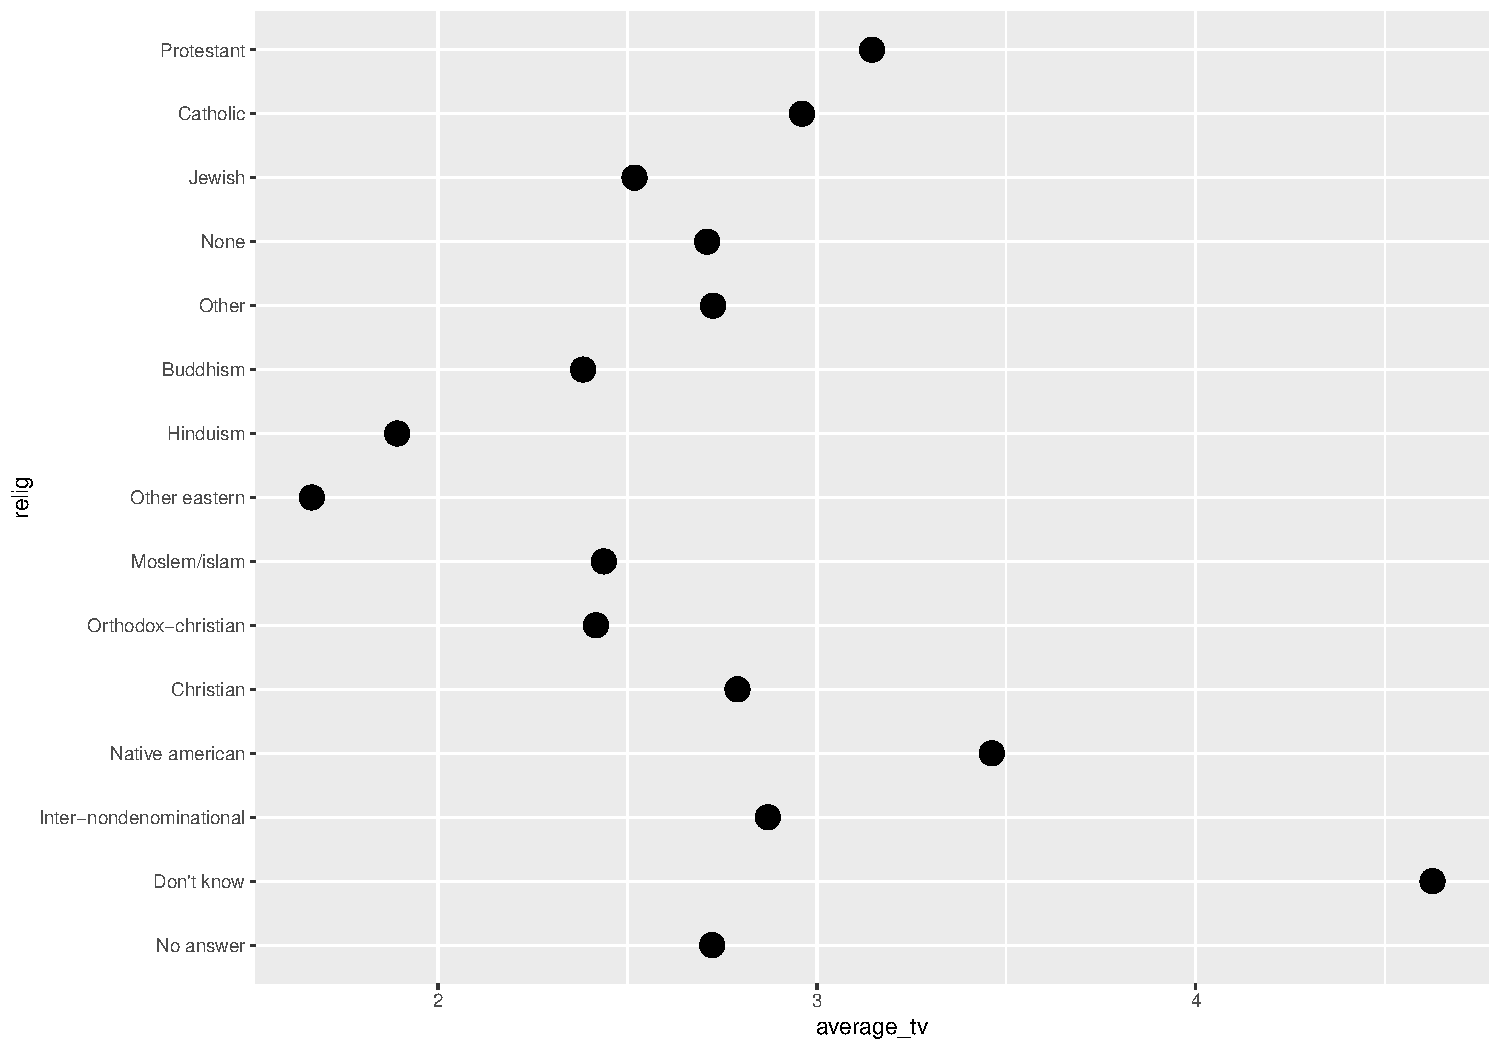
\includegraphics{gss_cat_files/figure-beamer/unnamed-chunk-1-1.pdf}

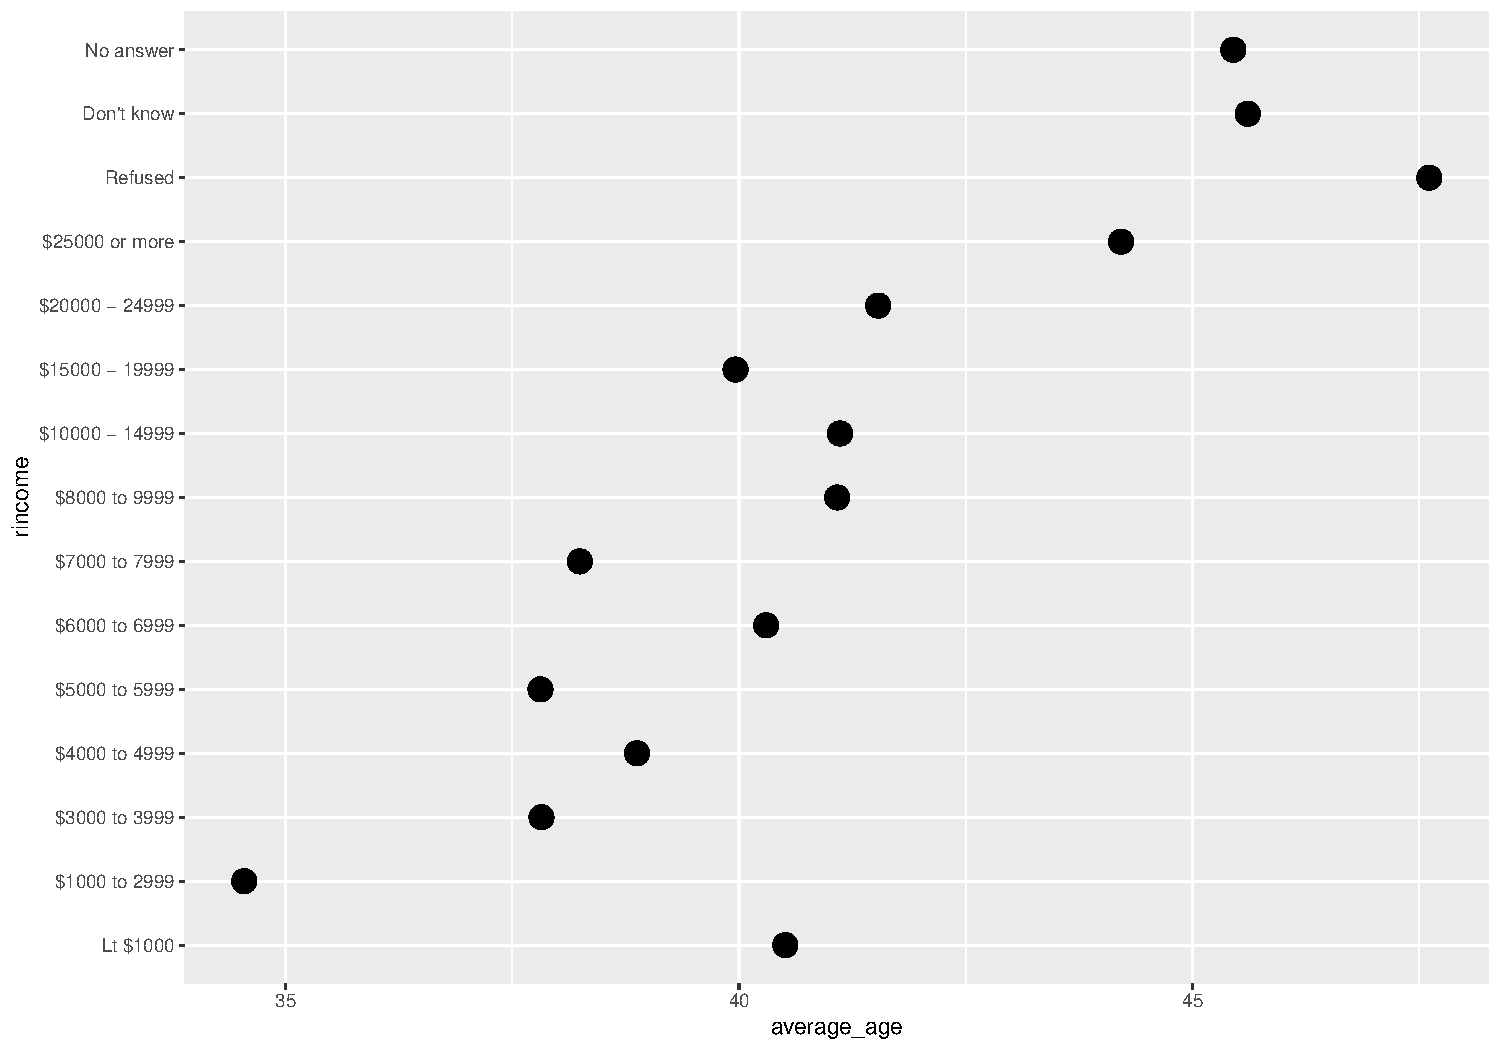
\includegraphics{gss_cat_files/figure-beamer/unnamed-chunk-1-2.pdf}

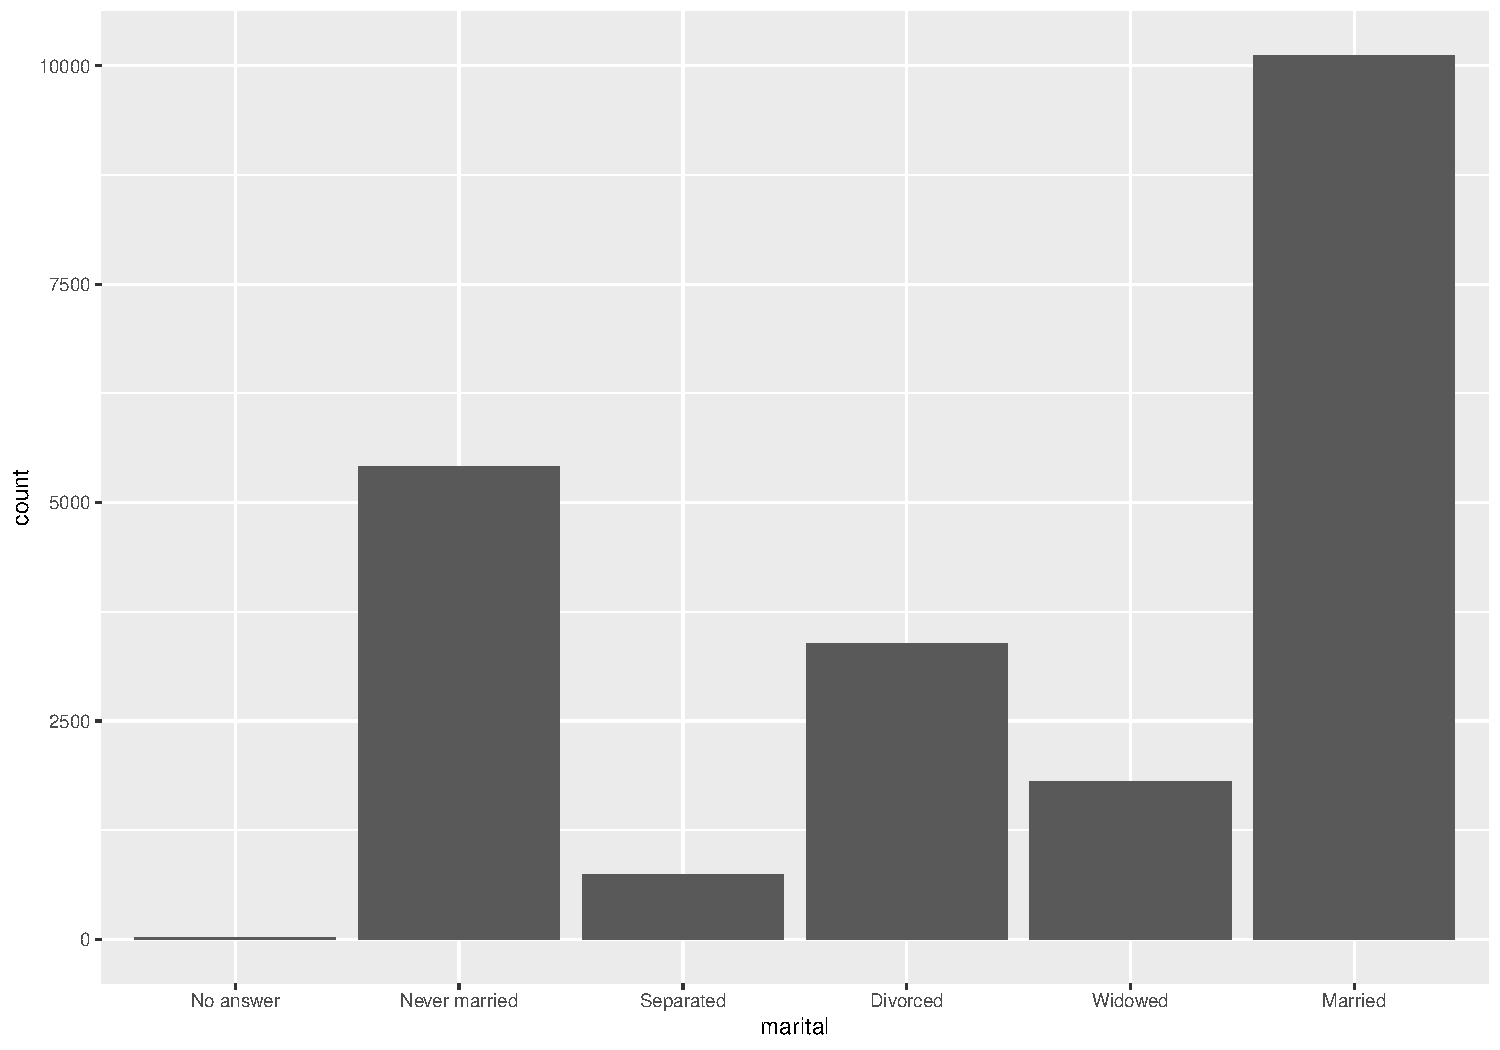
\includegraphics{gss_cat_files/figure-beamer/unnamed-chunk-1-3.pdf}

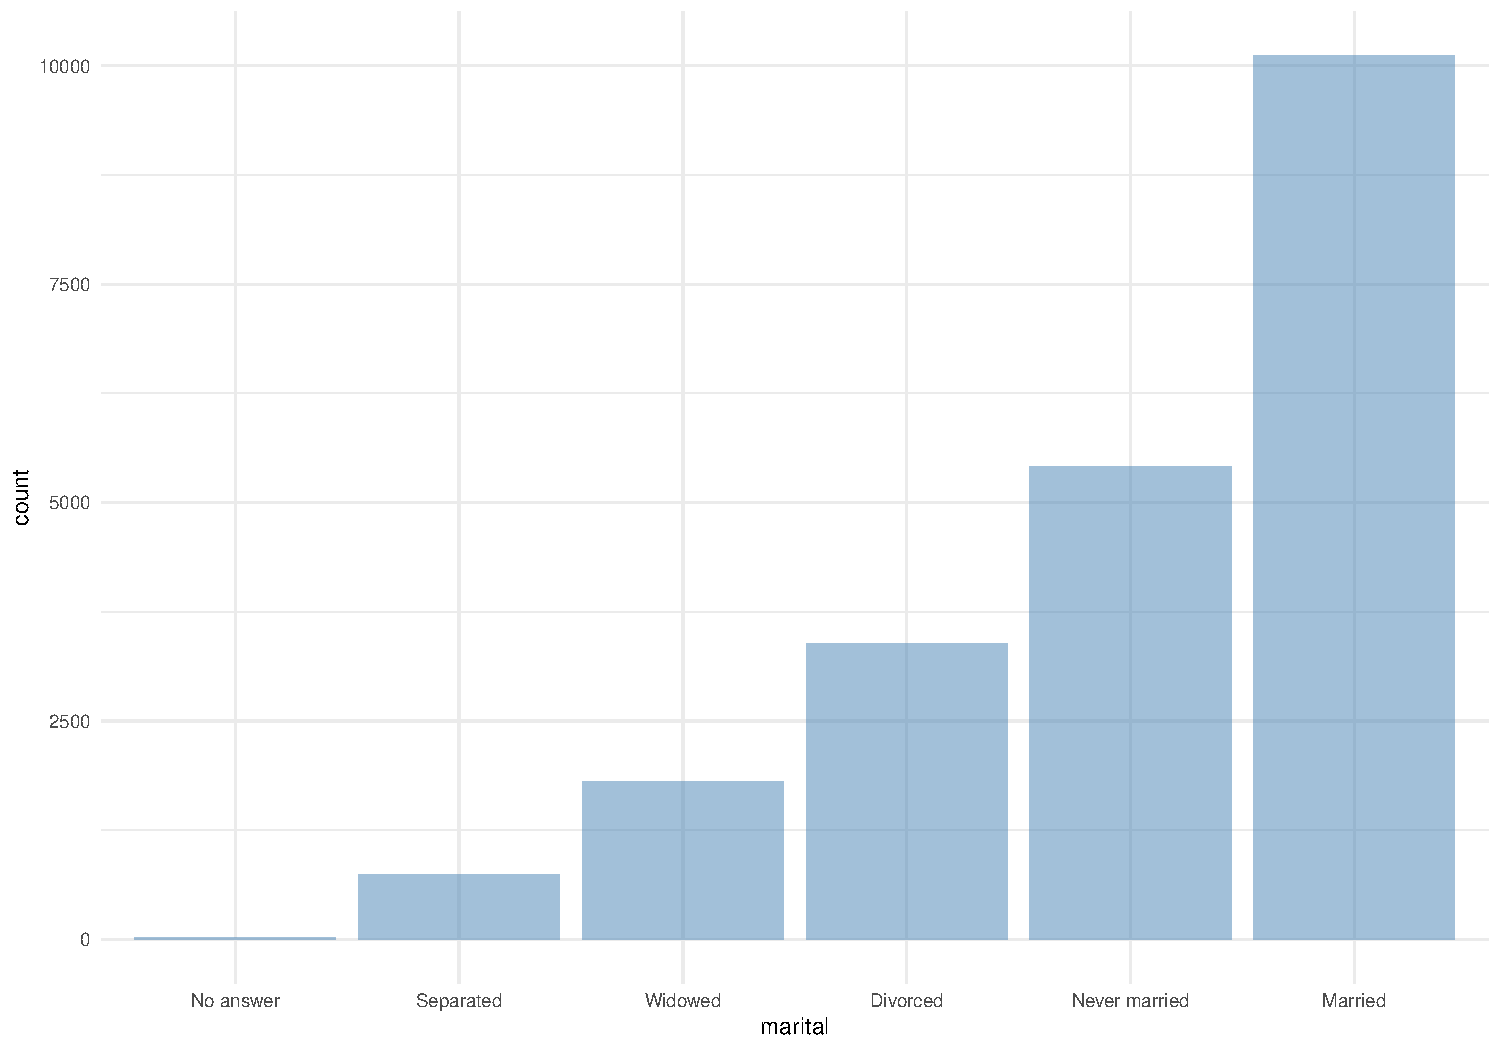
\includegraphics{gss_cat_files/figure-beamer/unnamed-chunk-1-4.pdf}

\begin{verbatim}
# A tibble: 8 x 2
  partyid                   n
  <fct>                 <int>
1 Other                   548
2 Republican, Strong     2314
3 Republican, Weak       3032
4 Independent, Near Rep  1791
5 Independent            4119
6 Independent, Near Dem  2499
7 Democrat, Weak         3690
8 Democrat, Strong       3490
\end{verbatim}

\begin{verbatim}
# A tibble: 4 x 2
  partyid     n
  <fct>   <int>
1 Other     548
2 Rep      7137
3 Ind      4119
4 Dem      9679
\end{verbatim}

\begin{verbatim}
# A tibble: 15 x 2
   relig                       n
   <fct>                   <int>
 1 Protestant              10846
 2 Catholic                 5124
 3 None                     3523
 4 Christian                 689
 5 Jewish                    388
 6 Other                     224
 7 Buddhism                  147
 8 Inter-nondenominational   109
 9 Moslem/islam              104
10 Orthodox-christian         95
11 No answer                  93
12 Hinduism                   71
13 Other eastern              32
14 Native american            23
15 Don't know                 15
\end{verbatim}

\begin{verbatim}
# A tibble: 3 x 2
  relig          n
  <fct>      <int>
1 Catholic    5124
2 Protestant 10846
3 Other       5513
\end{verbatim}

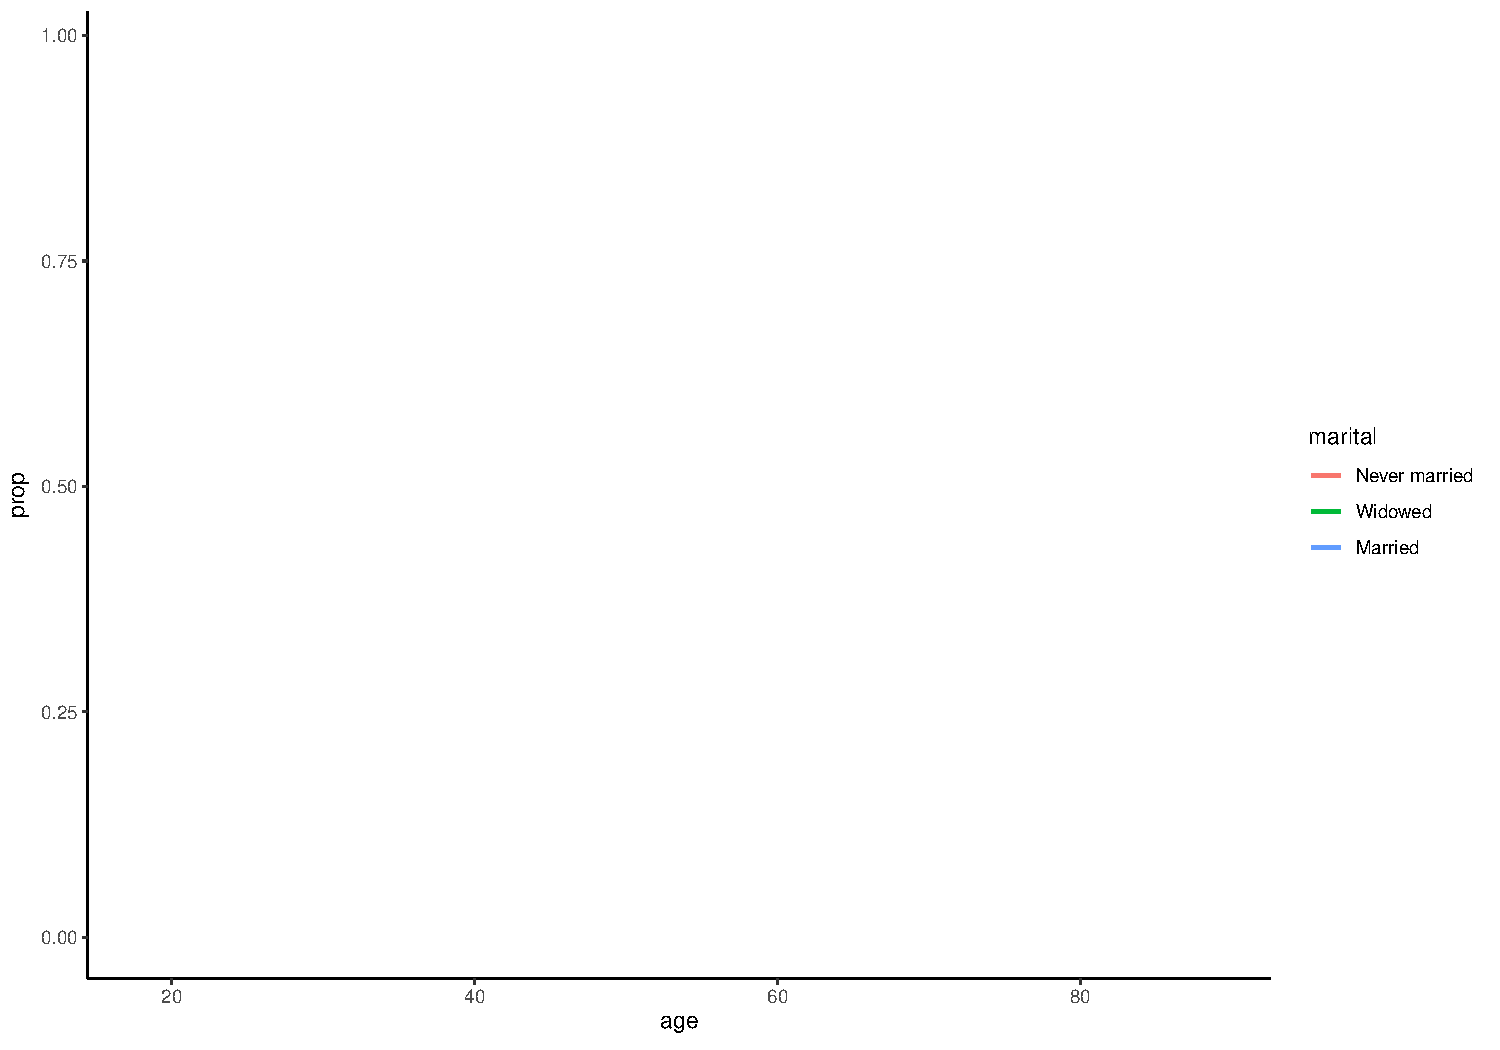
\includegraphics{gss_cat_files/figure-beamer/unnamed-chunk-1-5.pdf}

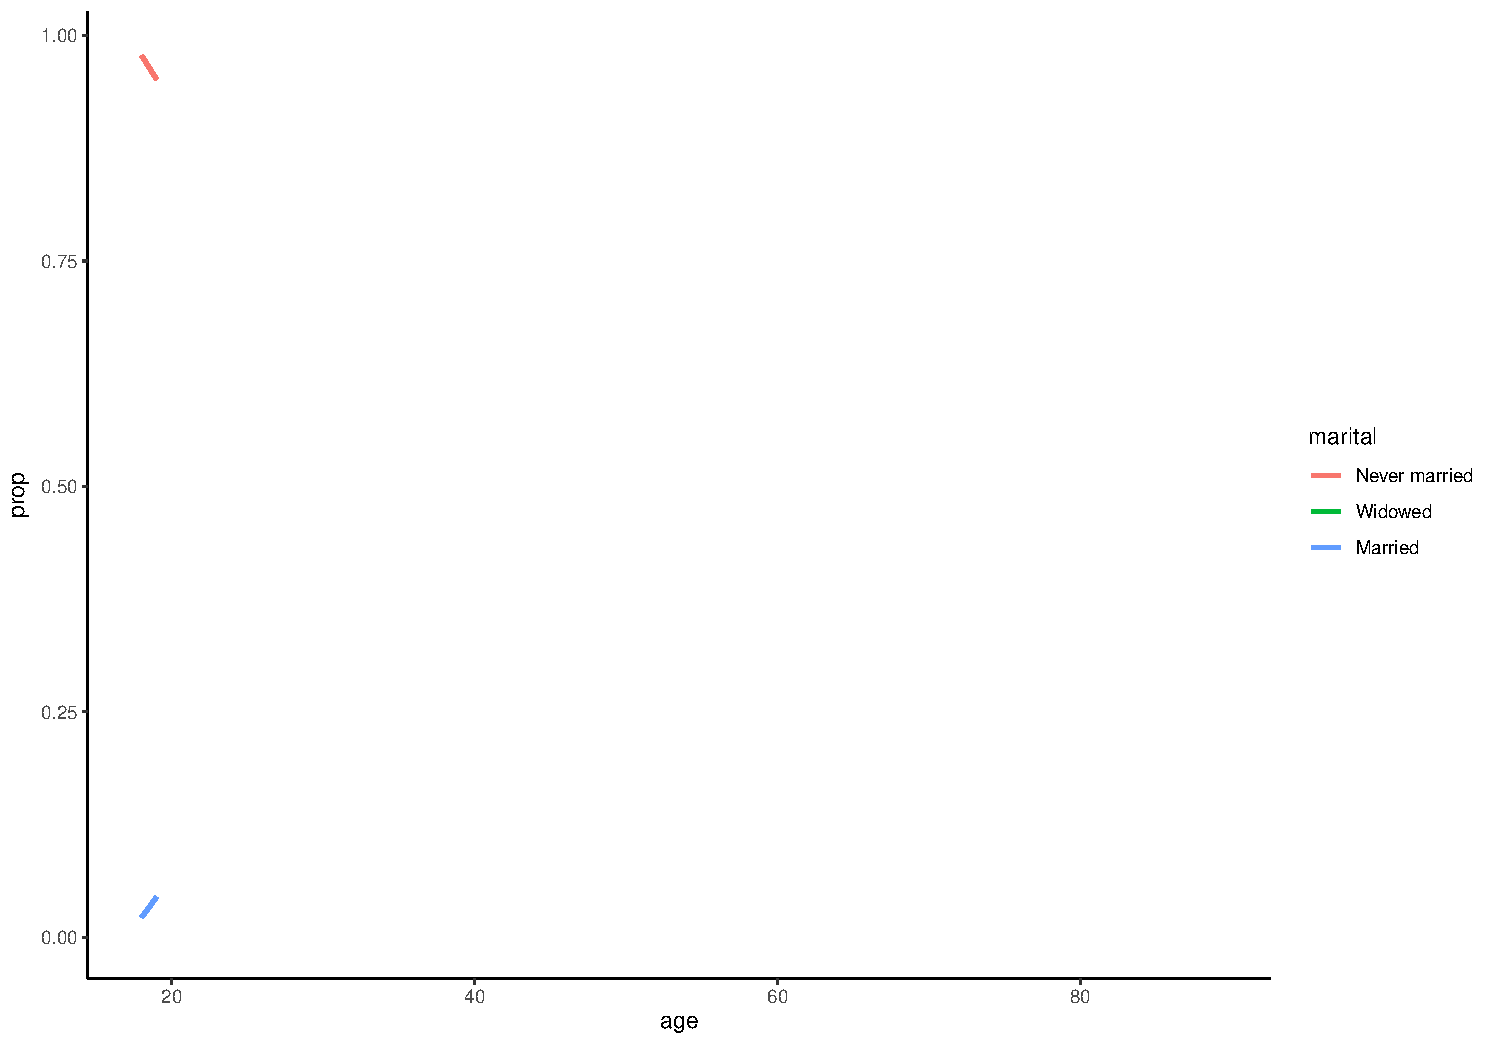
\includegraphics{gss_cat_files/figure-beamer/unnamed-chunk-1-6.pdf}

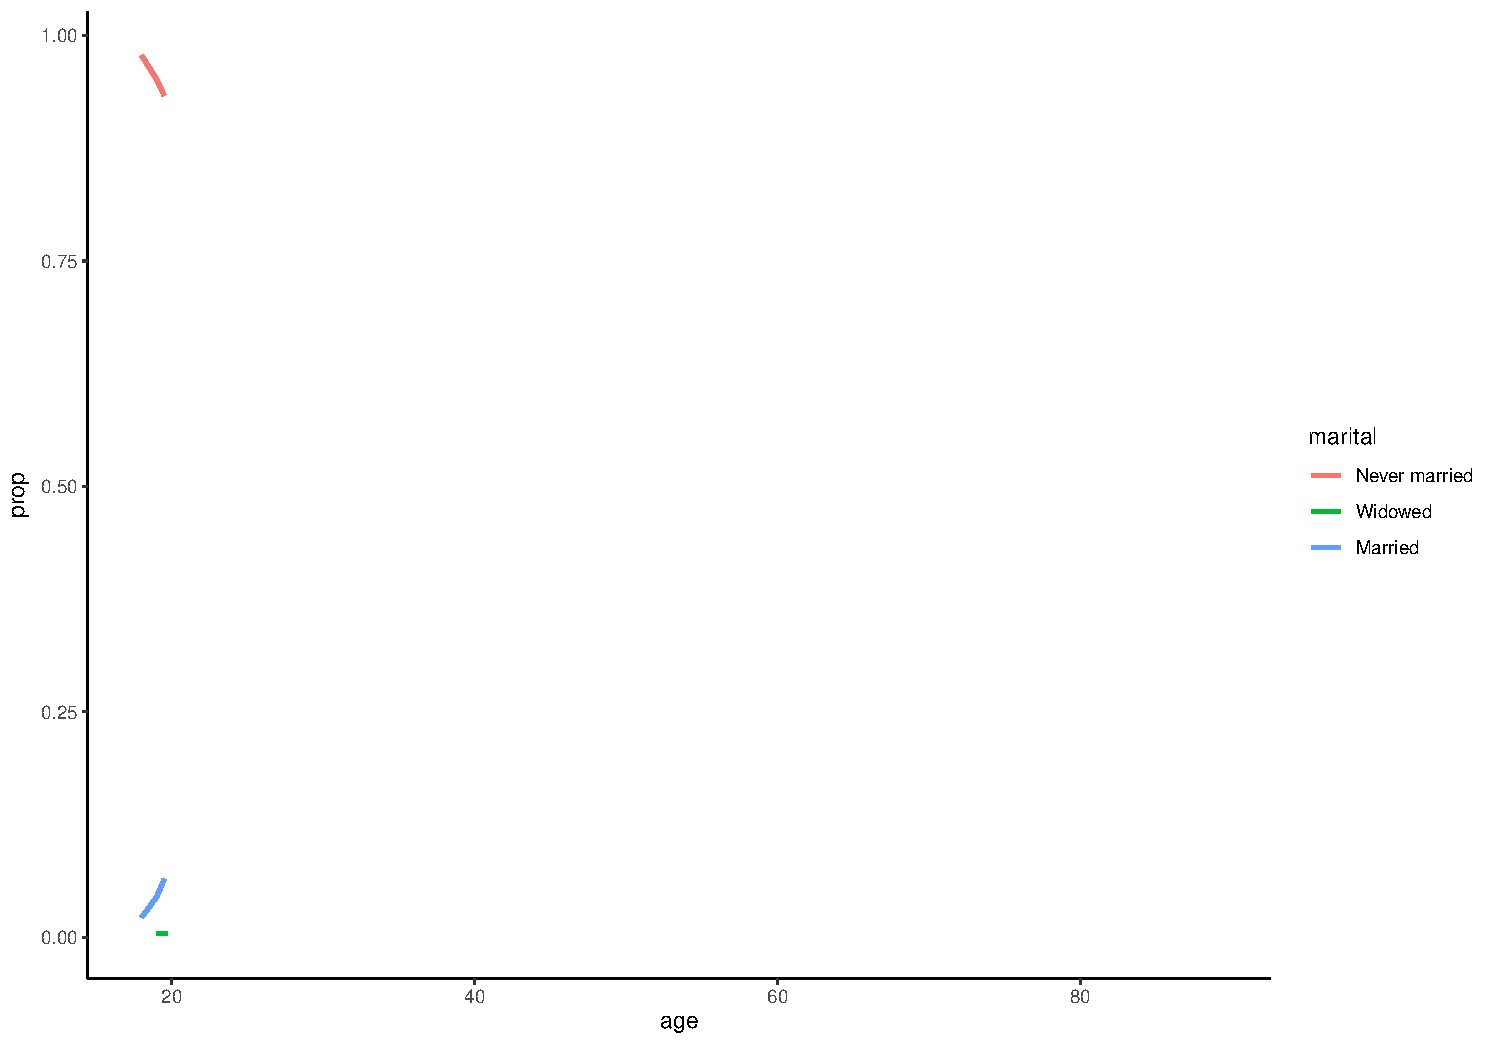
\includegraphics{gss_cat_files/figure-beamer/unnamed-chunk-1-7.pdf}

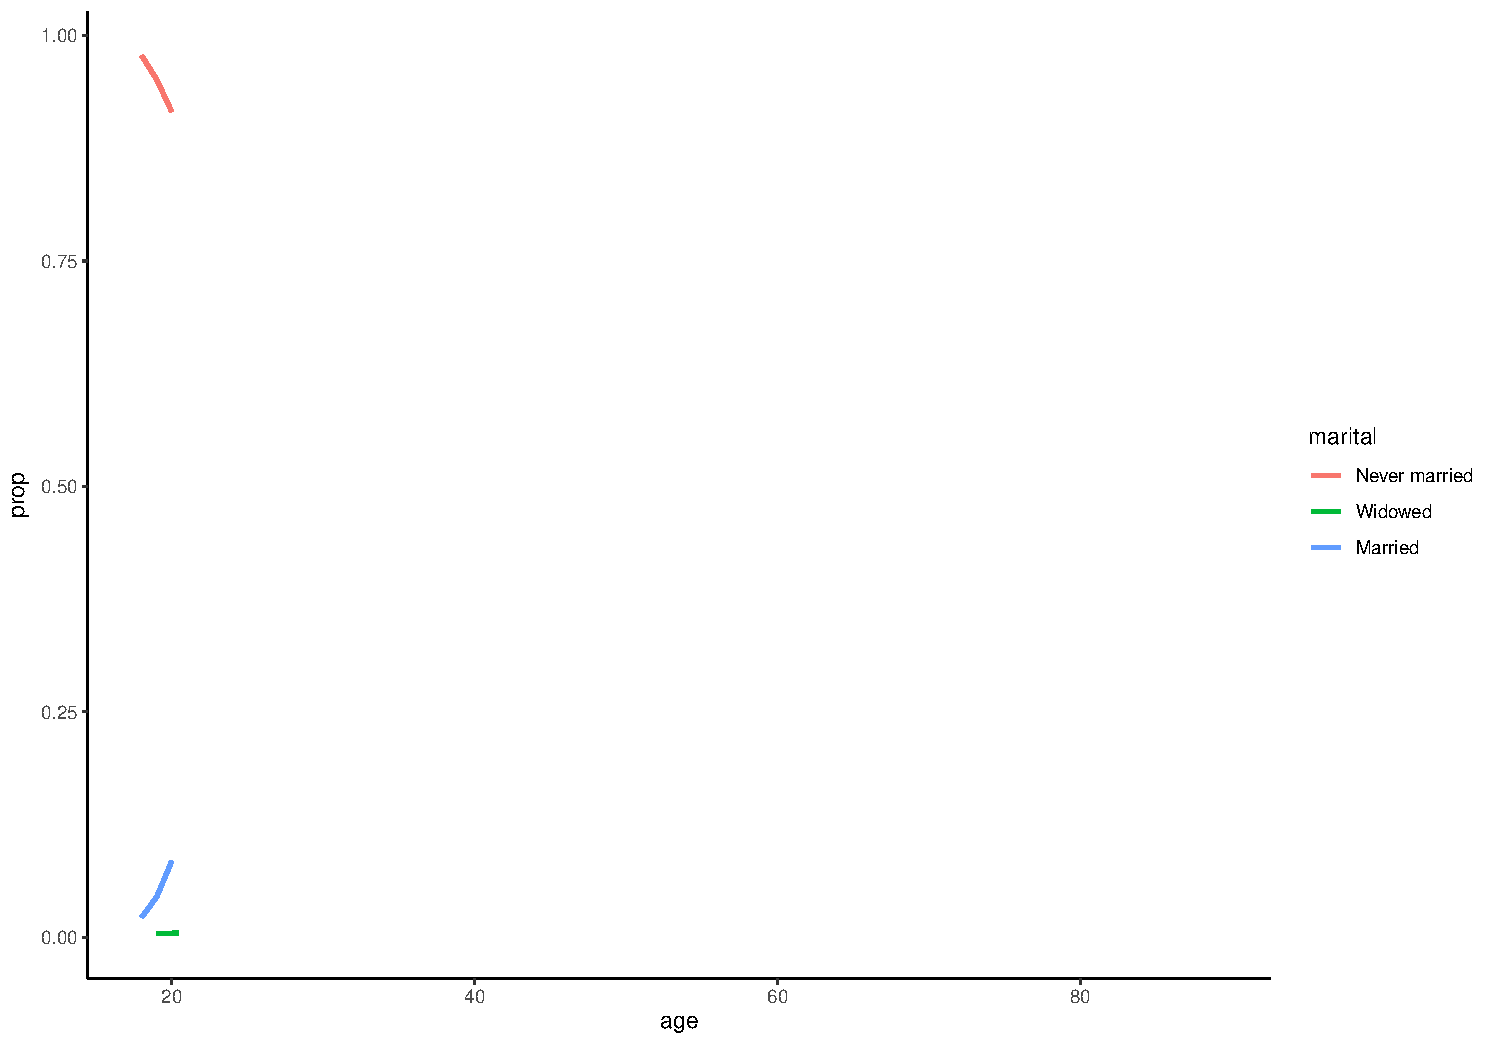
\includegraphics{gss_cat_files/figure-beamer/unnamed-chunk-1-8.pdf}

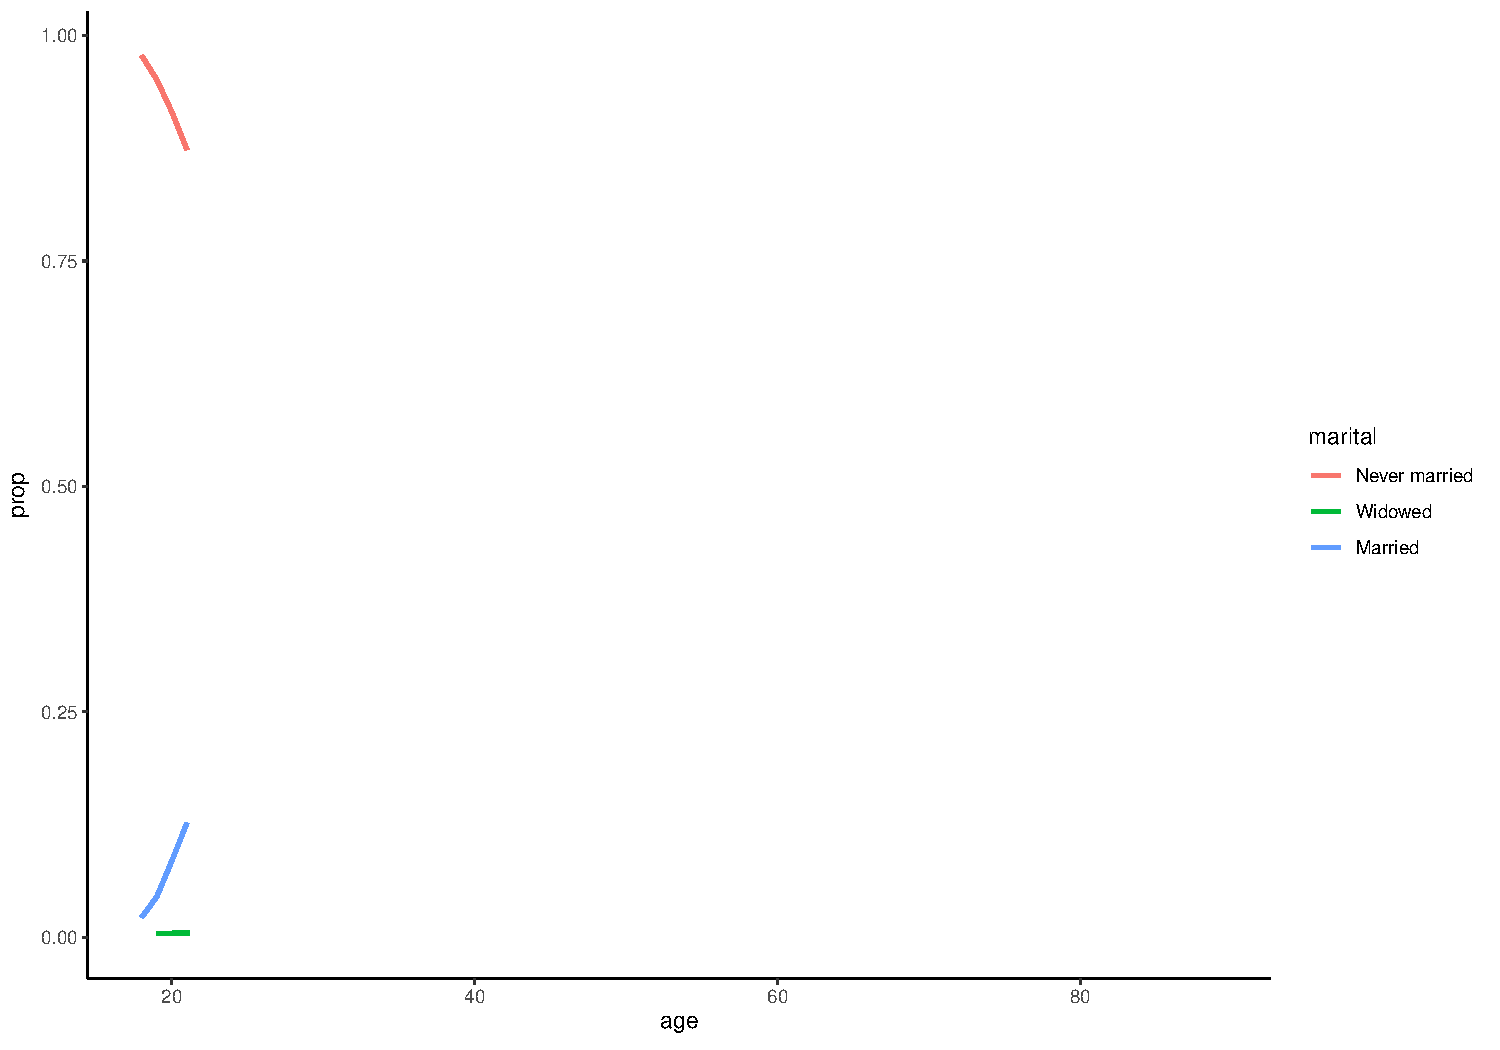
\includegraphics{gss_cat_files/figure-beamer/unnamed-chunk-1-9.pdf}

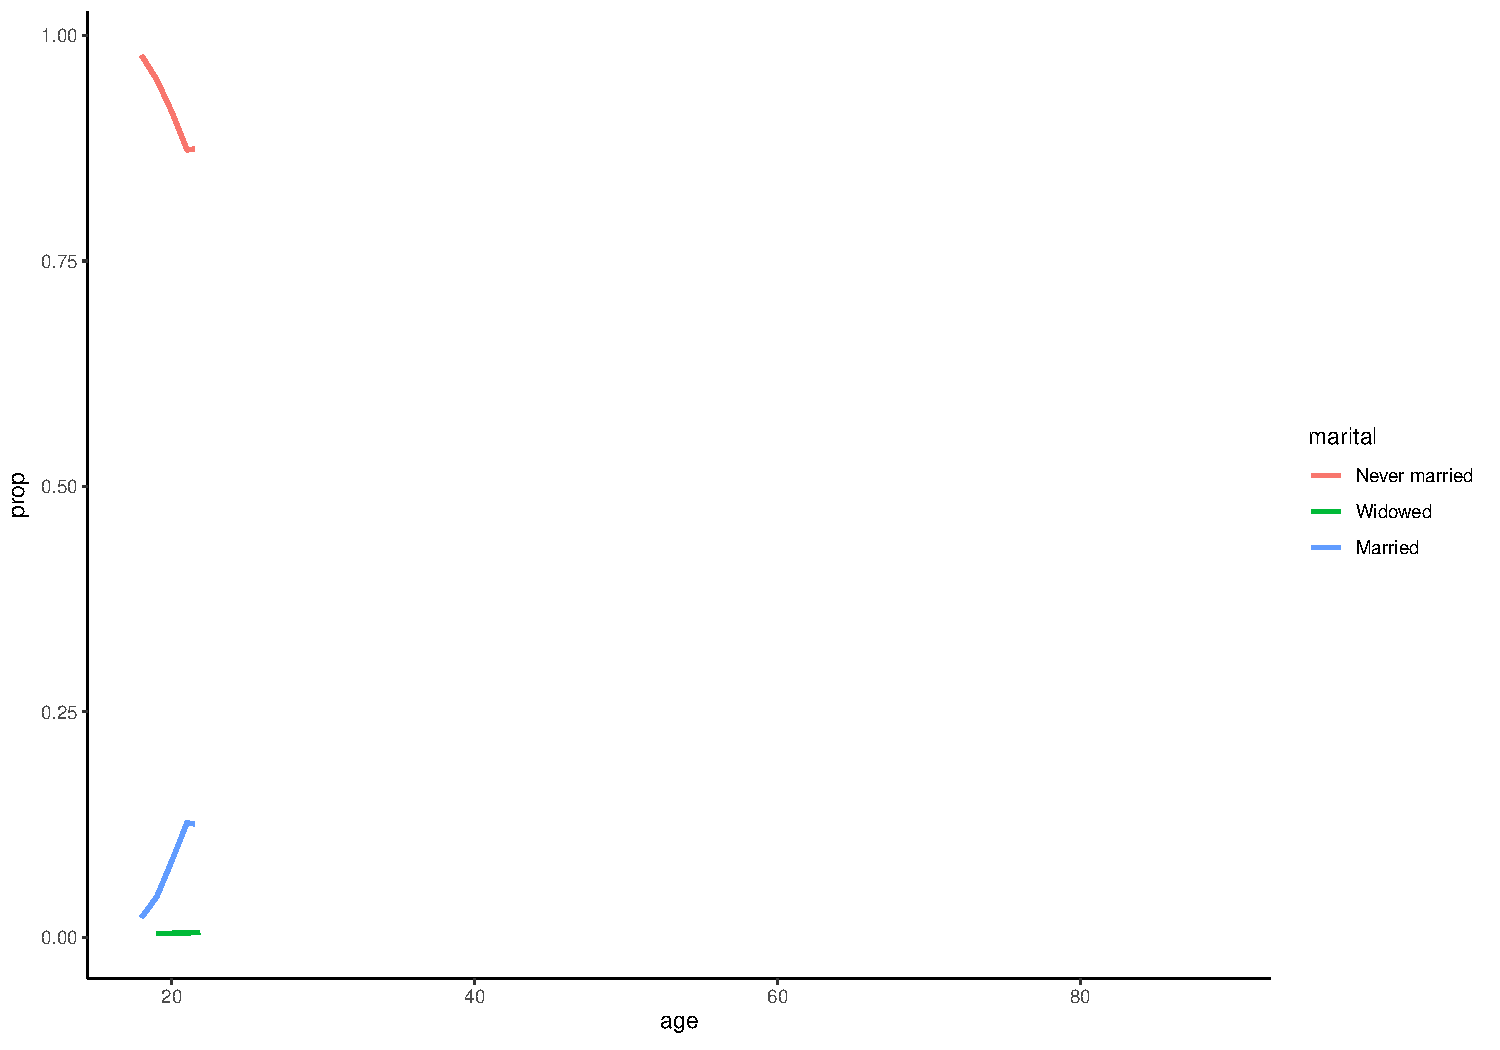
\includegraphics{gss_cat_files/figure-beamer/unnamed-chunk-1-10.pdf}

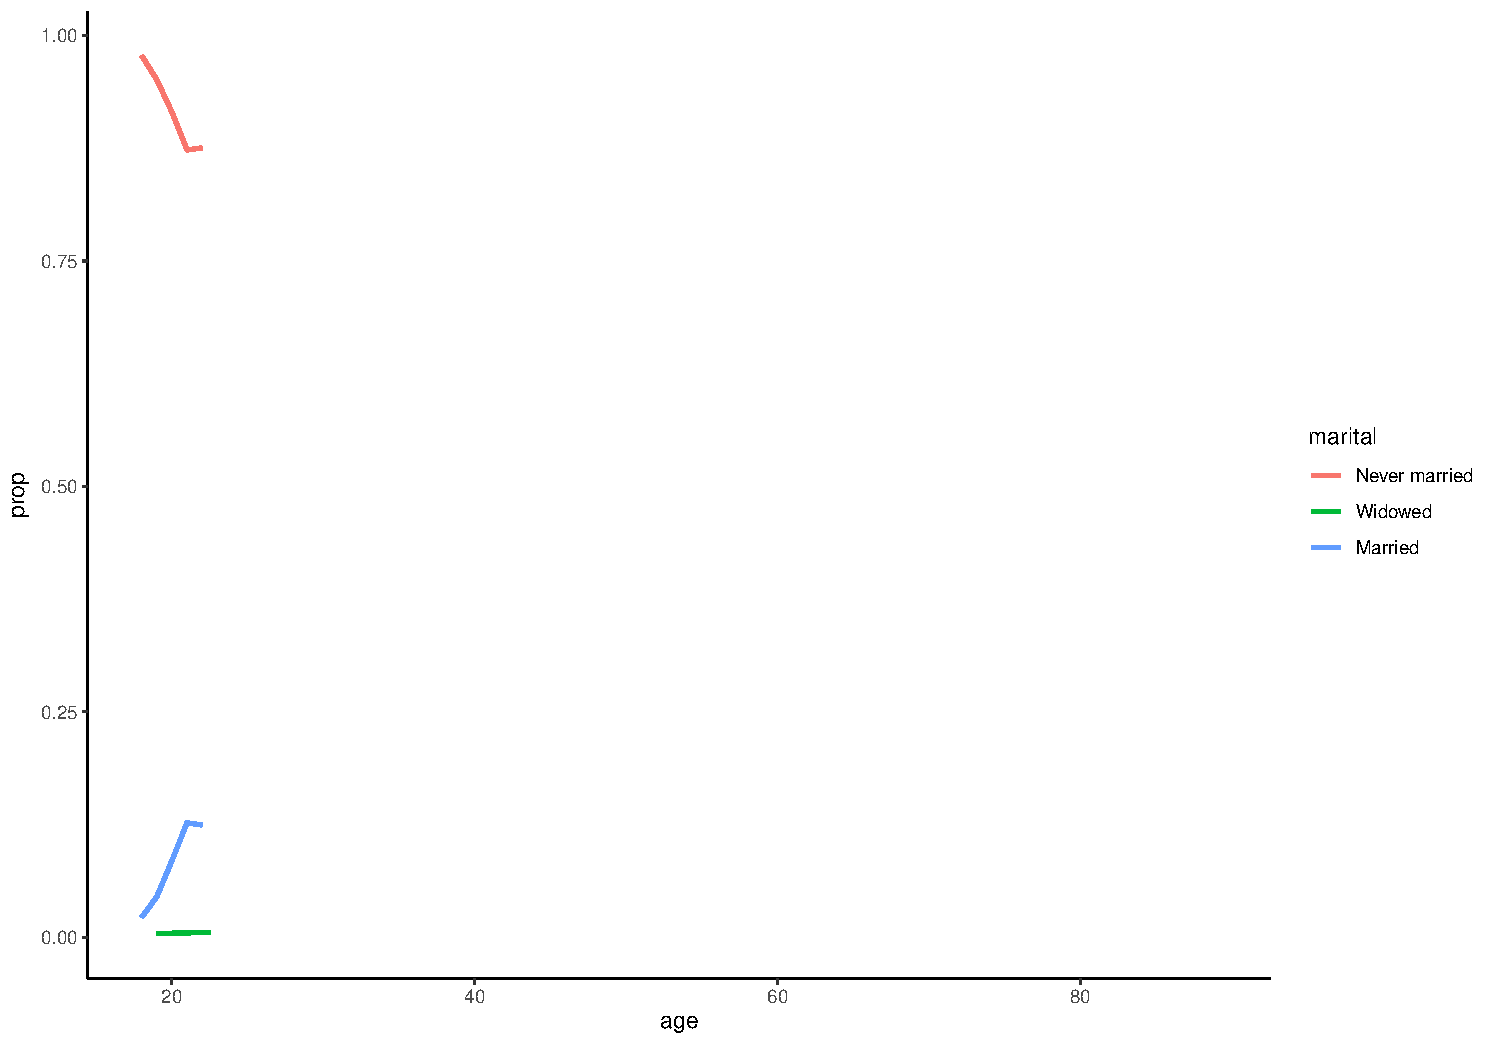
\includegraphics{gss_cat_files/figure-beamer/unnamed-chunk-1-11.pdf}

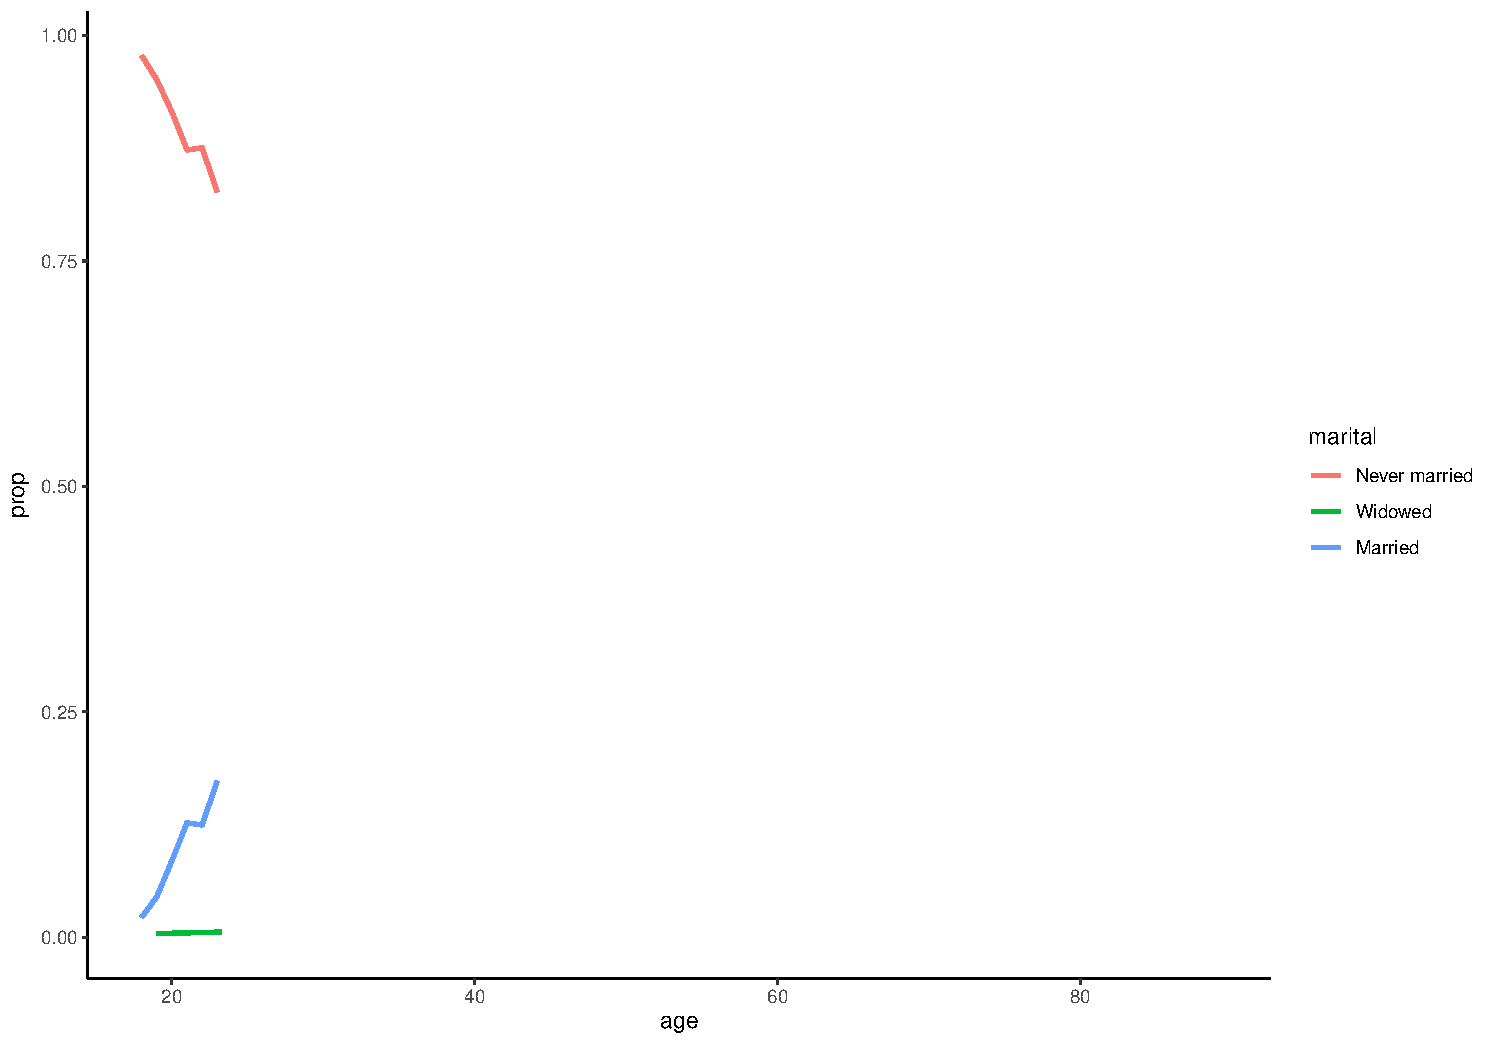
\includegraphics{gss_cat_files/figure-beamer/unnamed-chunk-1-12.pdf}

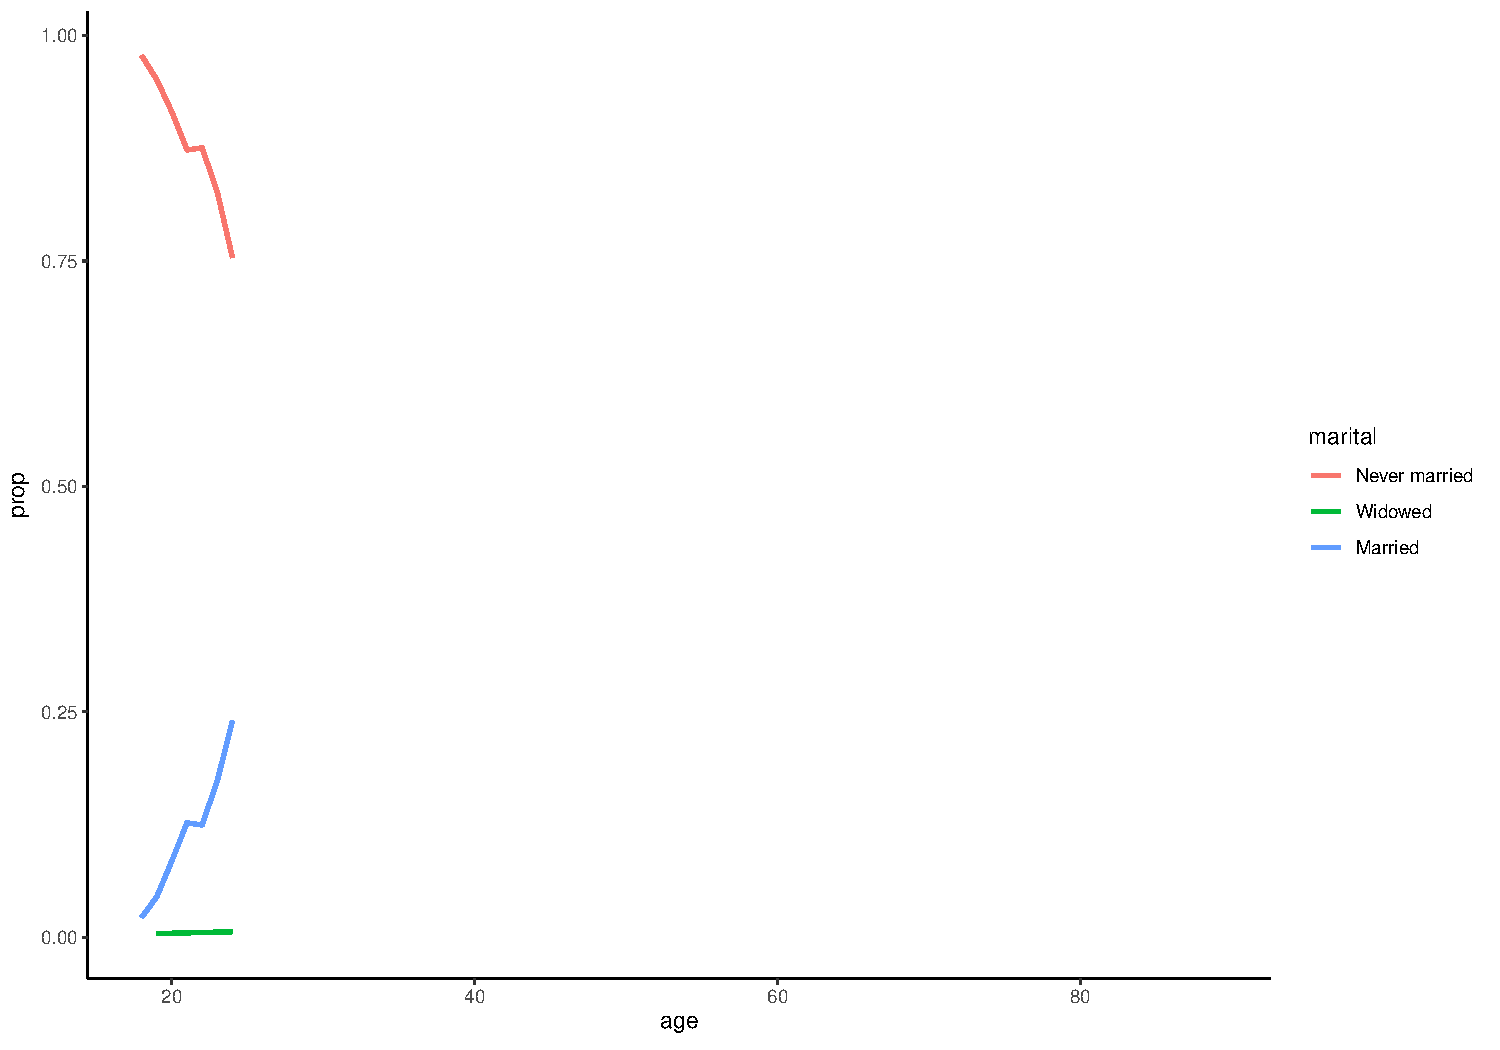
\includegraphics{gss_cat_files/figure-beamer/unnamed-chunk-1-13.pdf}

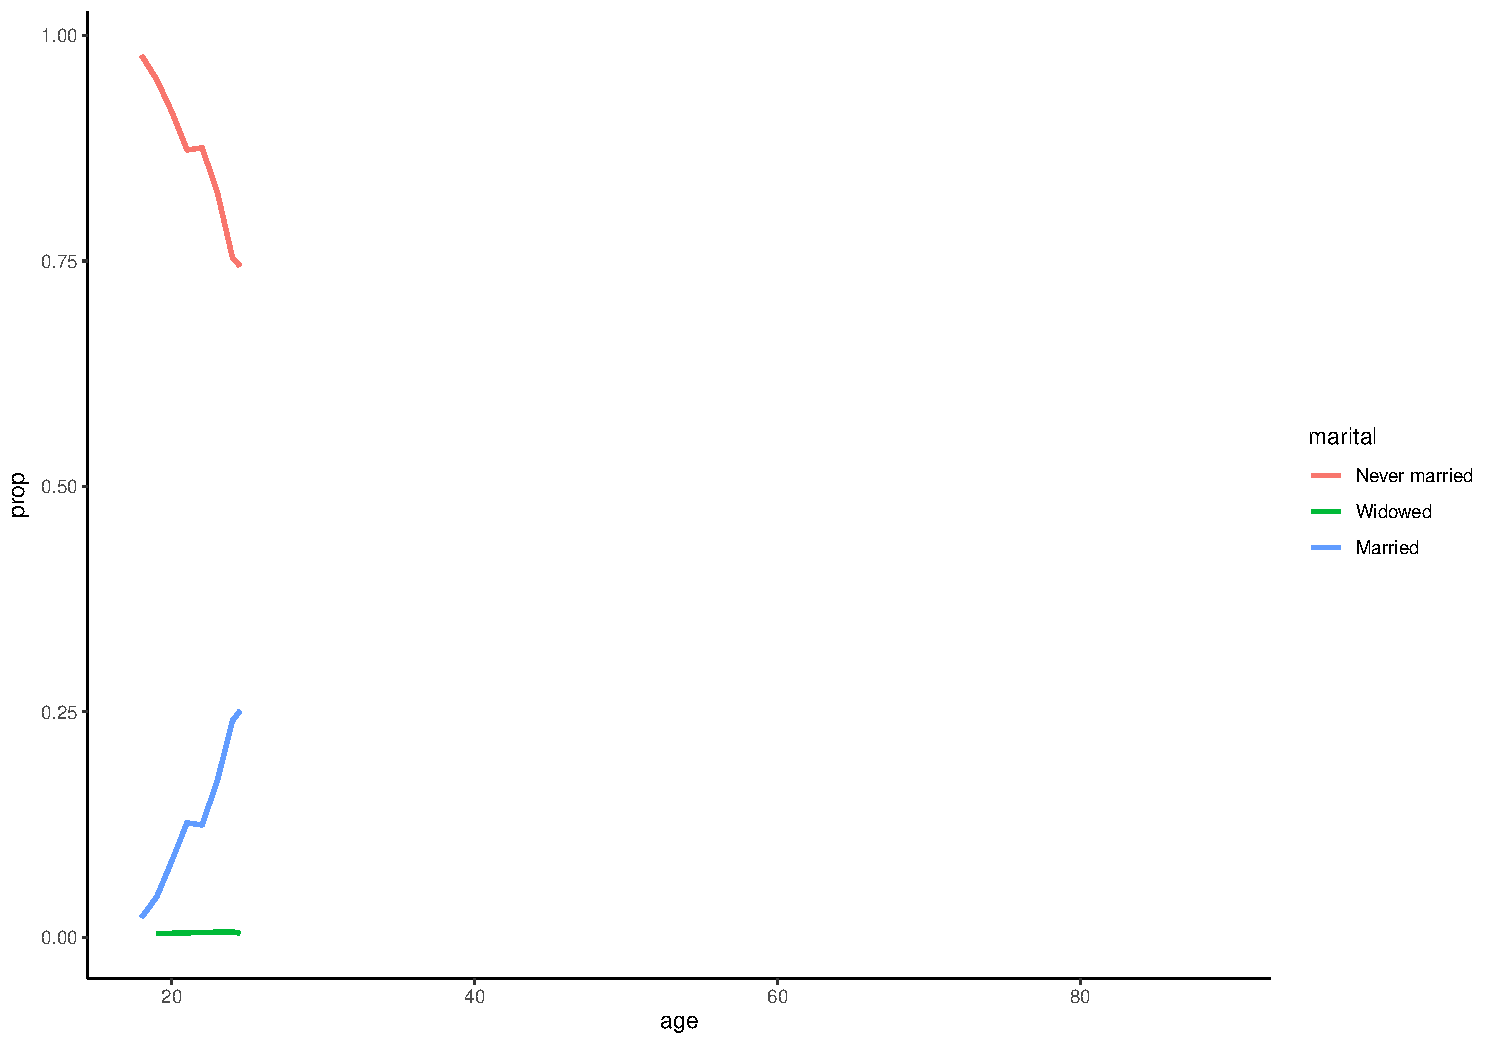
\includegraphics{gss_cat_files/figure-beamer/unnamed-chunk-1-14.pdf}

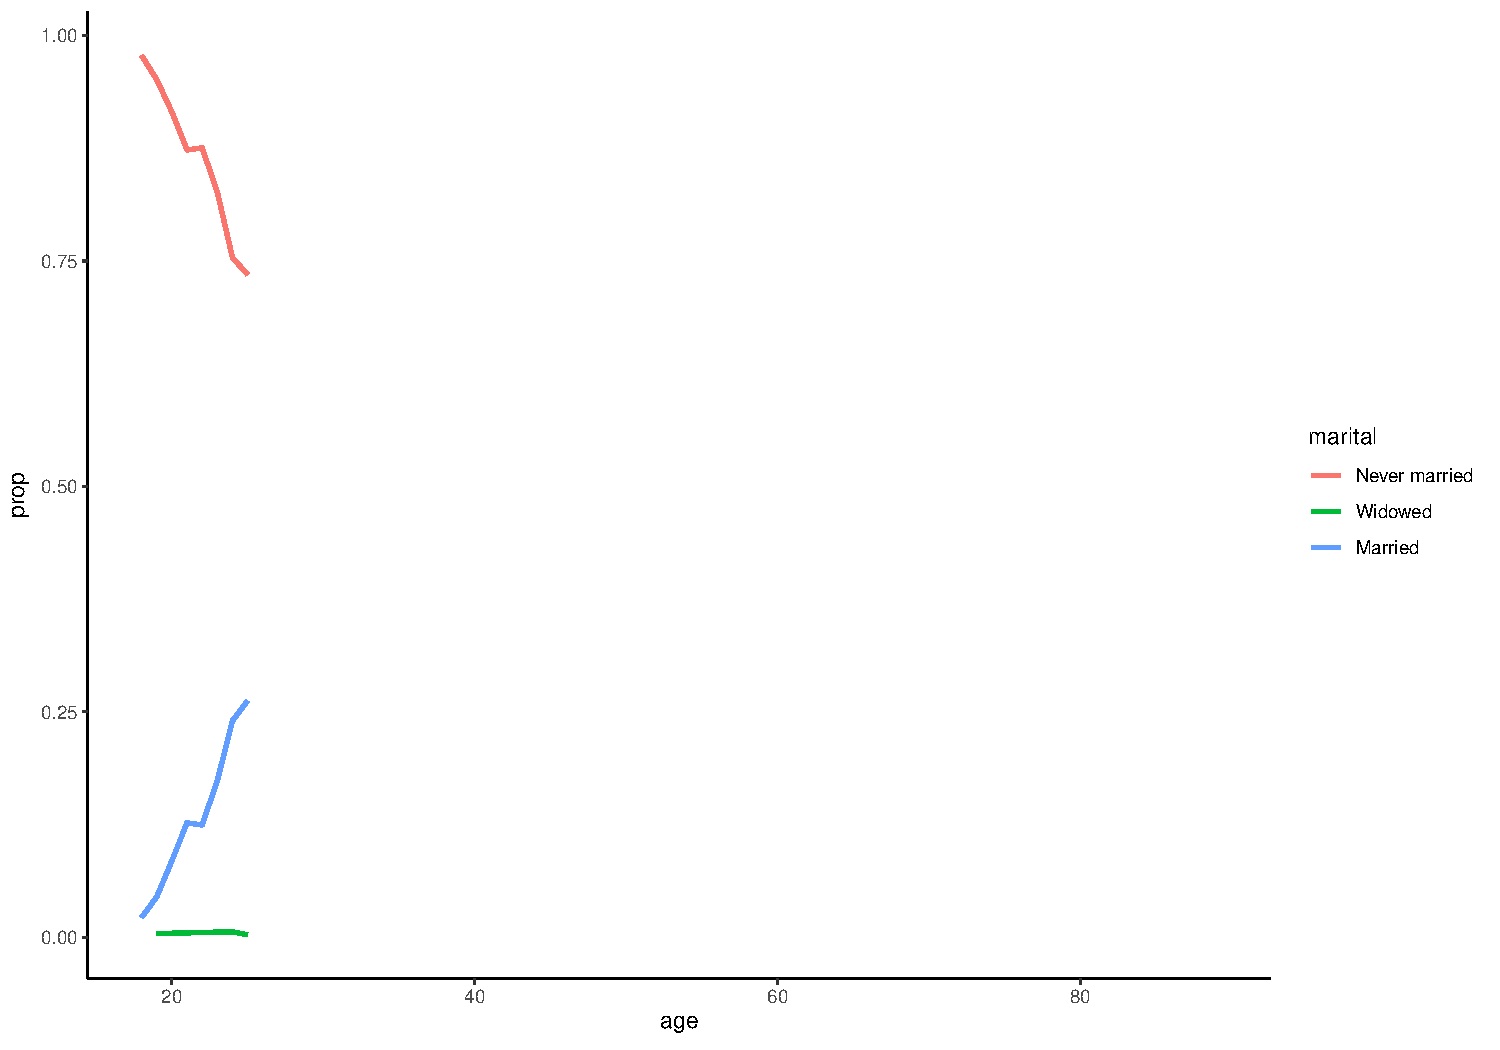
\includegraphics{gss_cat_files/figure-beamer/unnamed-chunk-1-15.pdf}

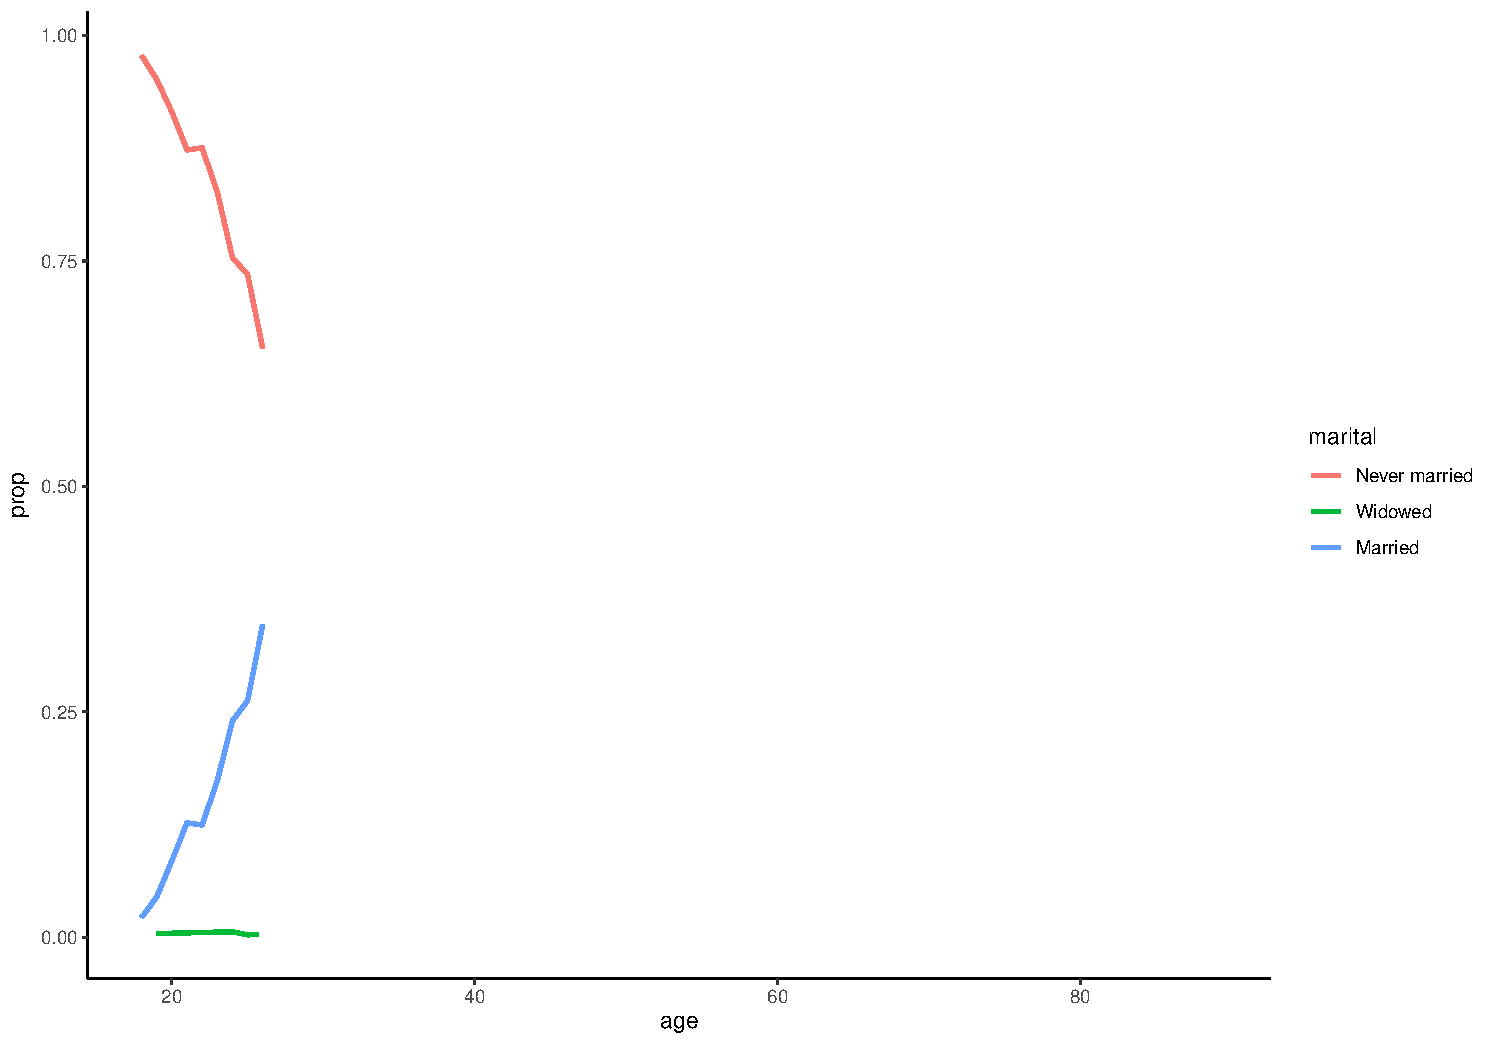
\includegraphics{gss_cat_files/figure-beamer/unnamed-chunk-1-16.pdf}

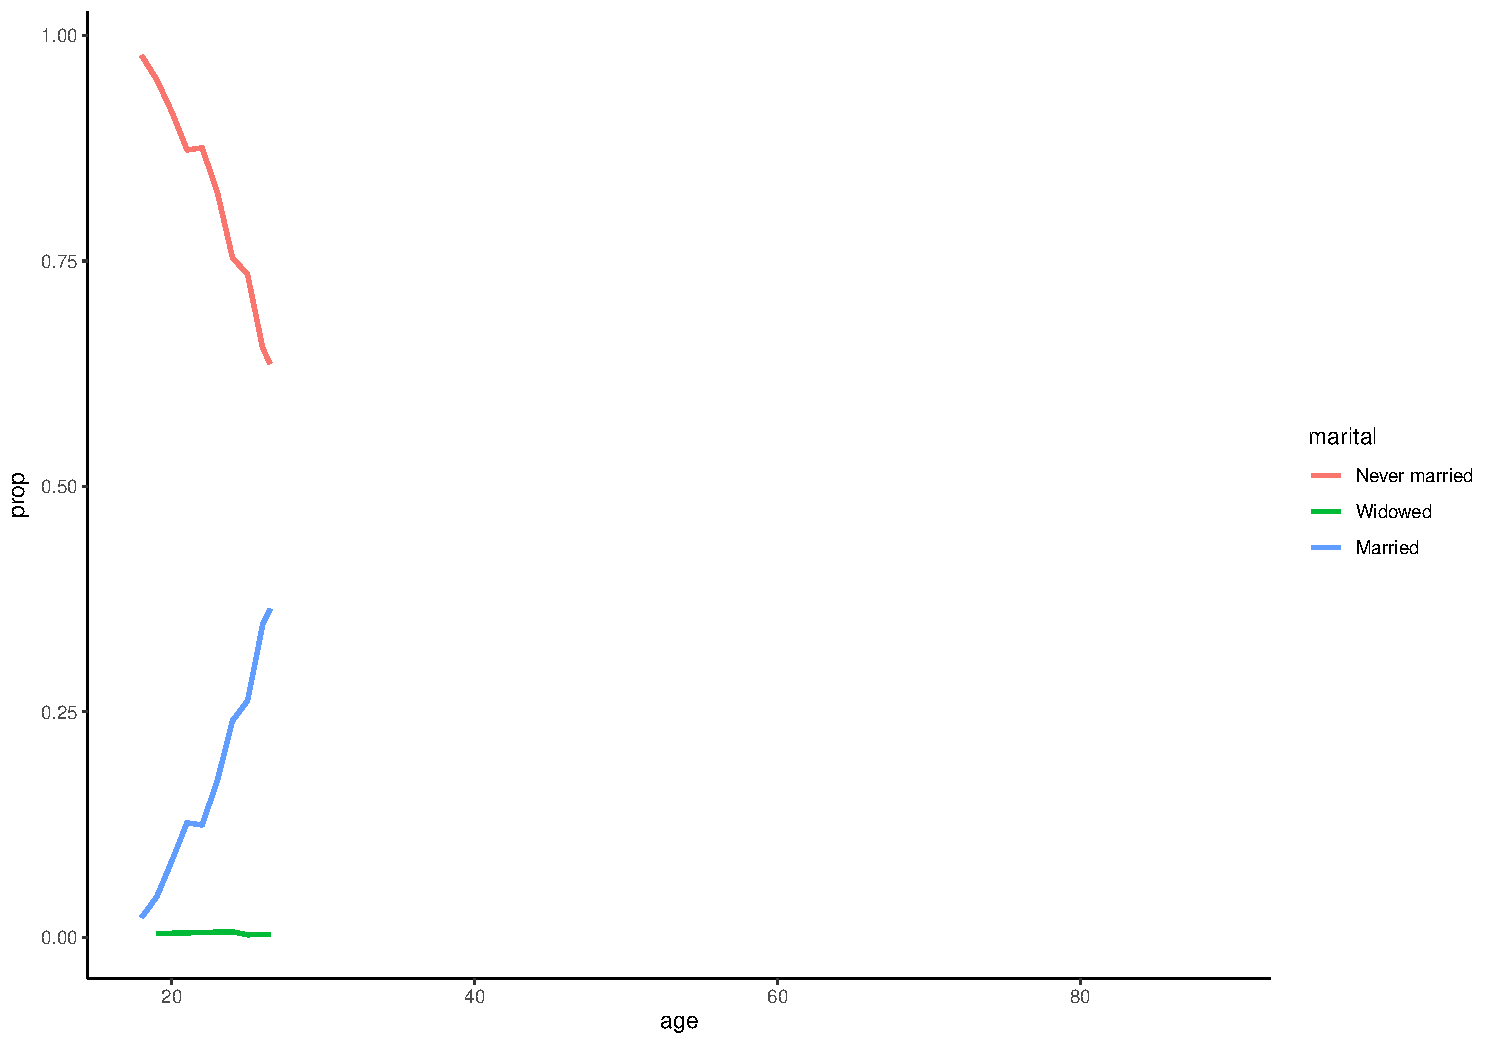
\includegraphics{gss_cat_files/figure-beamer/unnamed-chunk-1-17.pdf}

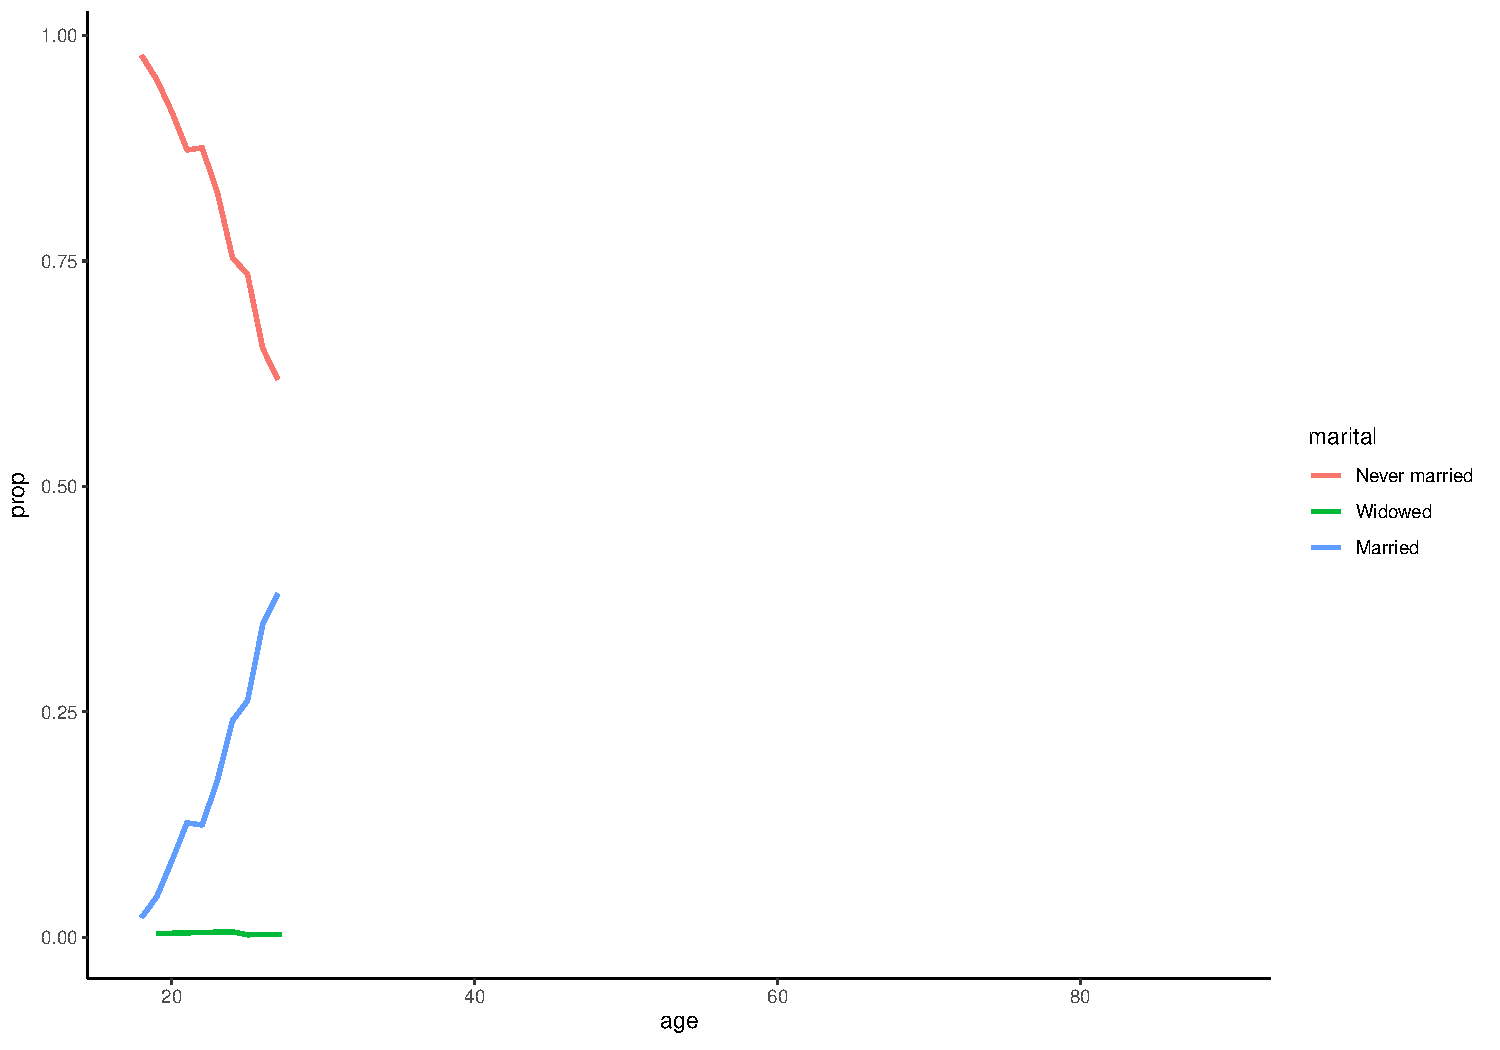
\includegraphics{gss_cat_files/figure-beamer/unnamed-chunk-1-18.pdf}

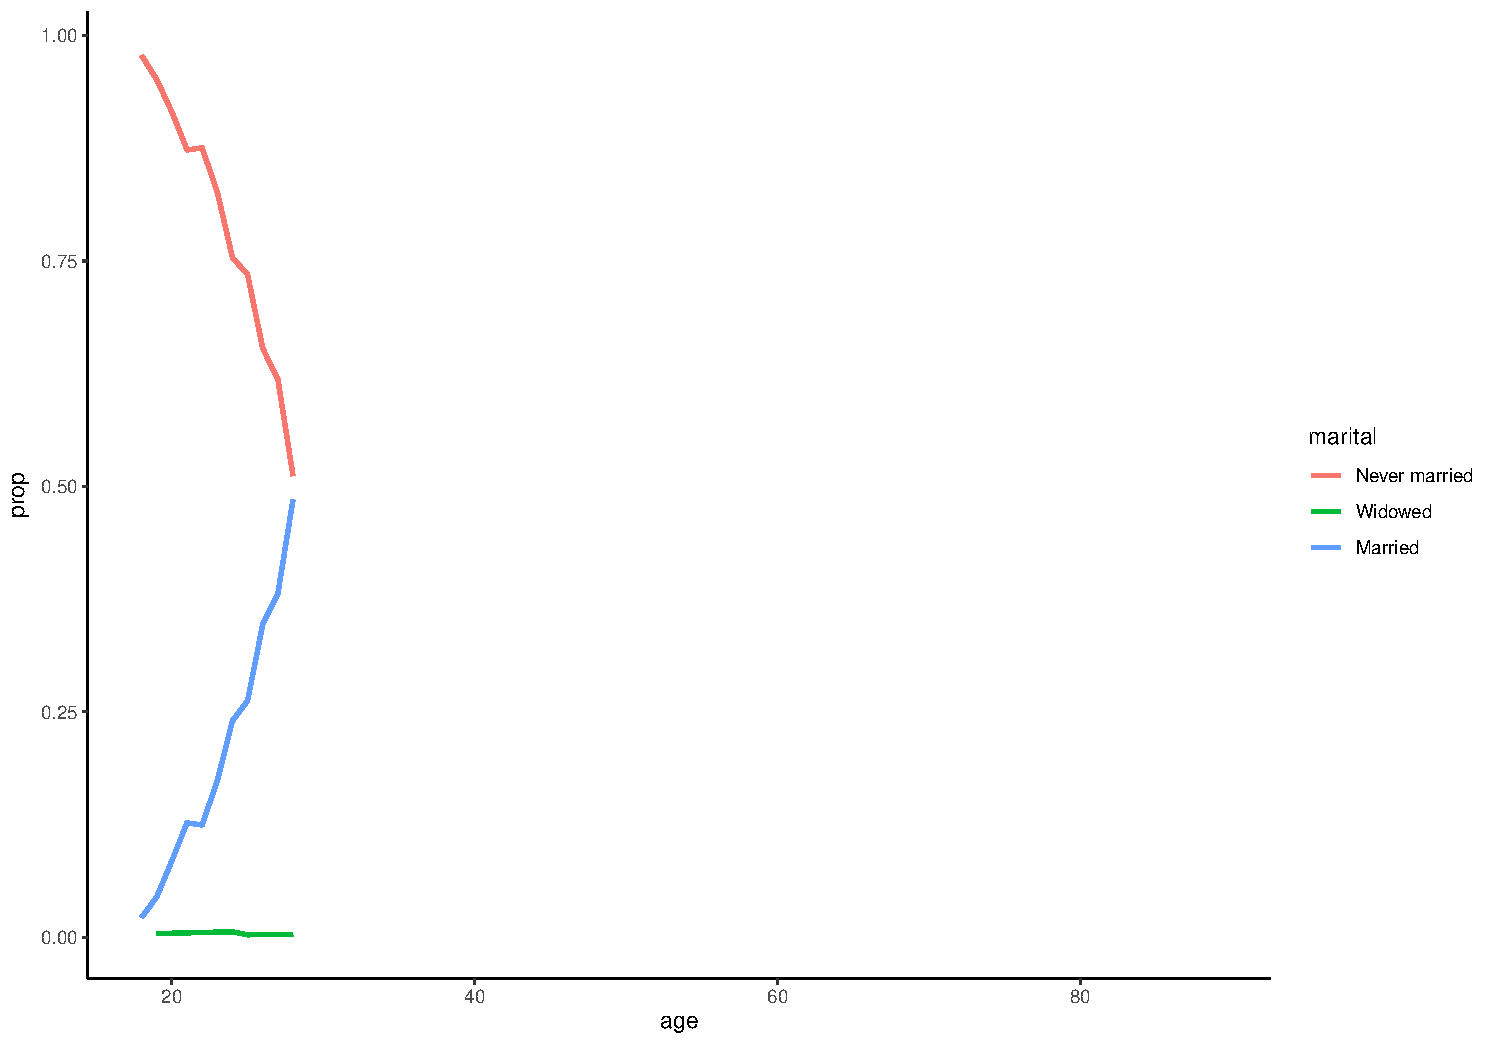
\includegraphics{gss_cat_files/figure-beamer/unnamed-chunk-1-19.pdf}

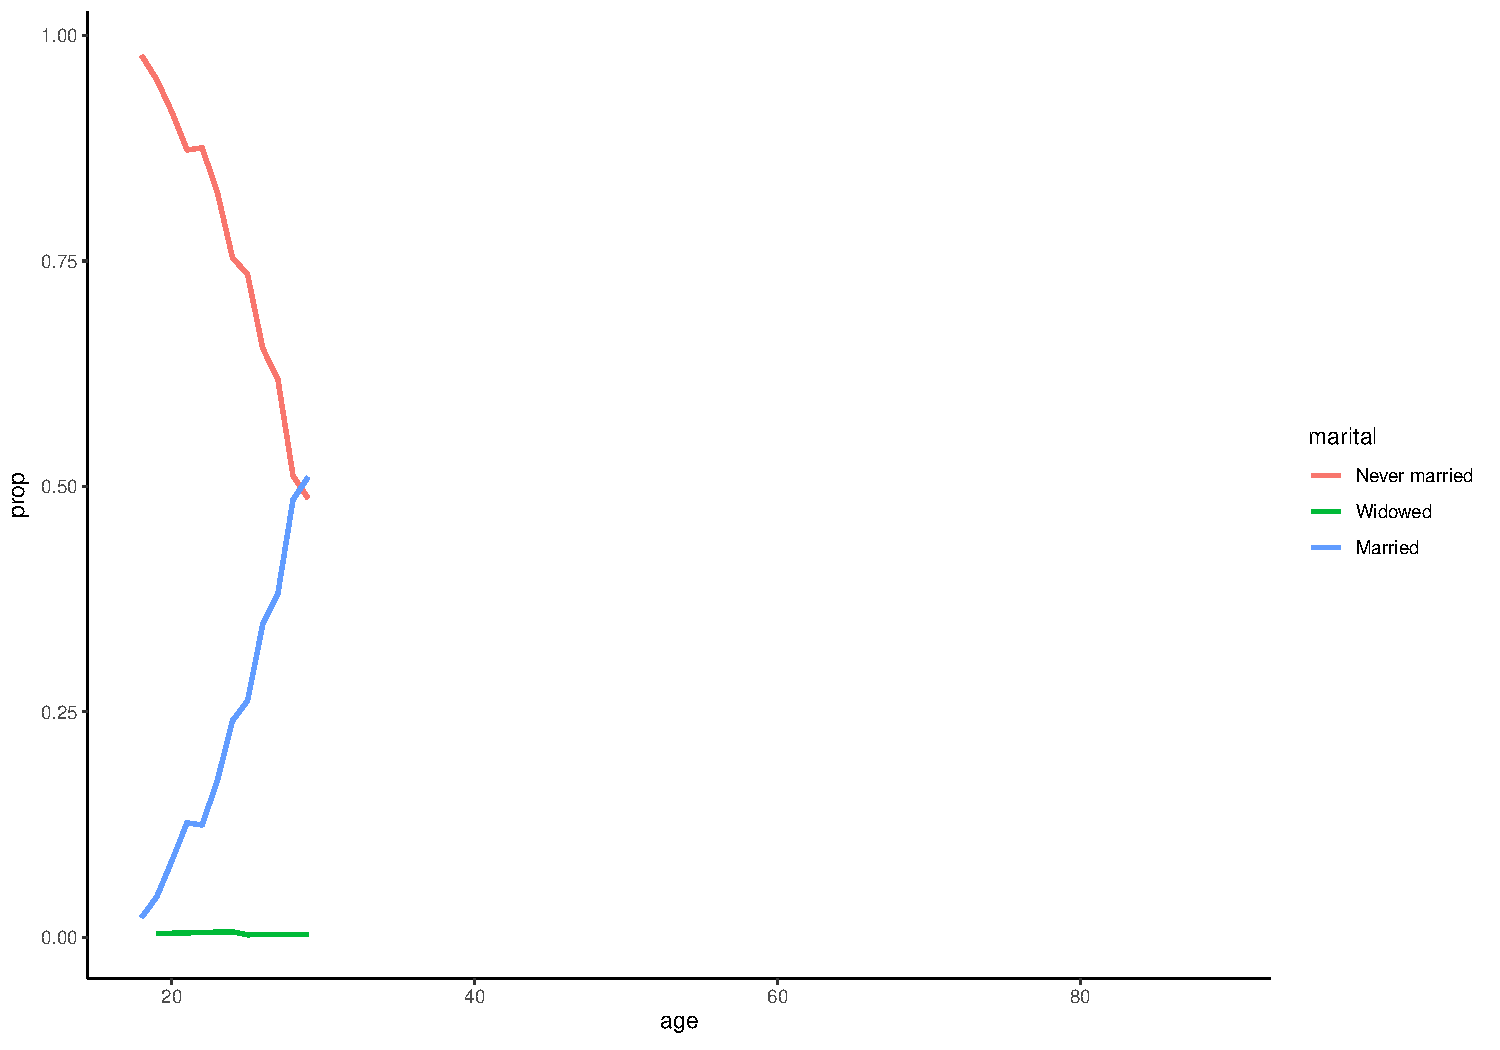
\includegraphics{gss_cat_files/figure-beamer/unnamed-chunk-1-20.pdf}

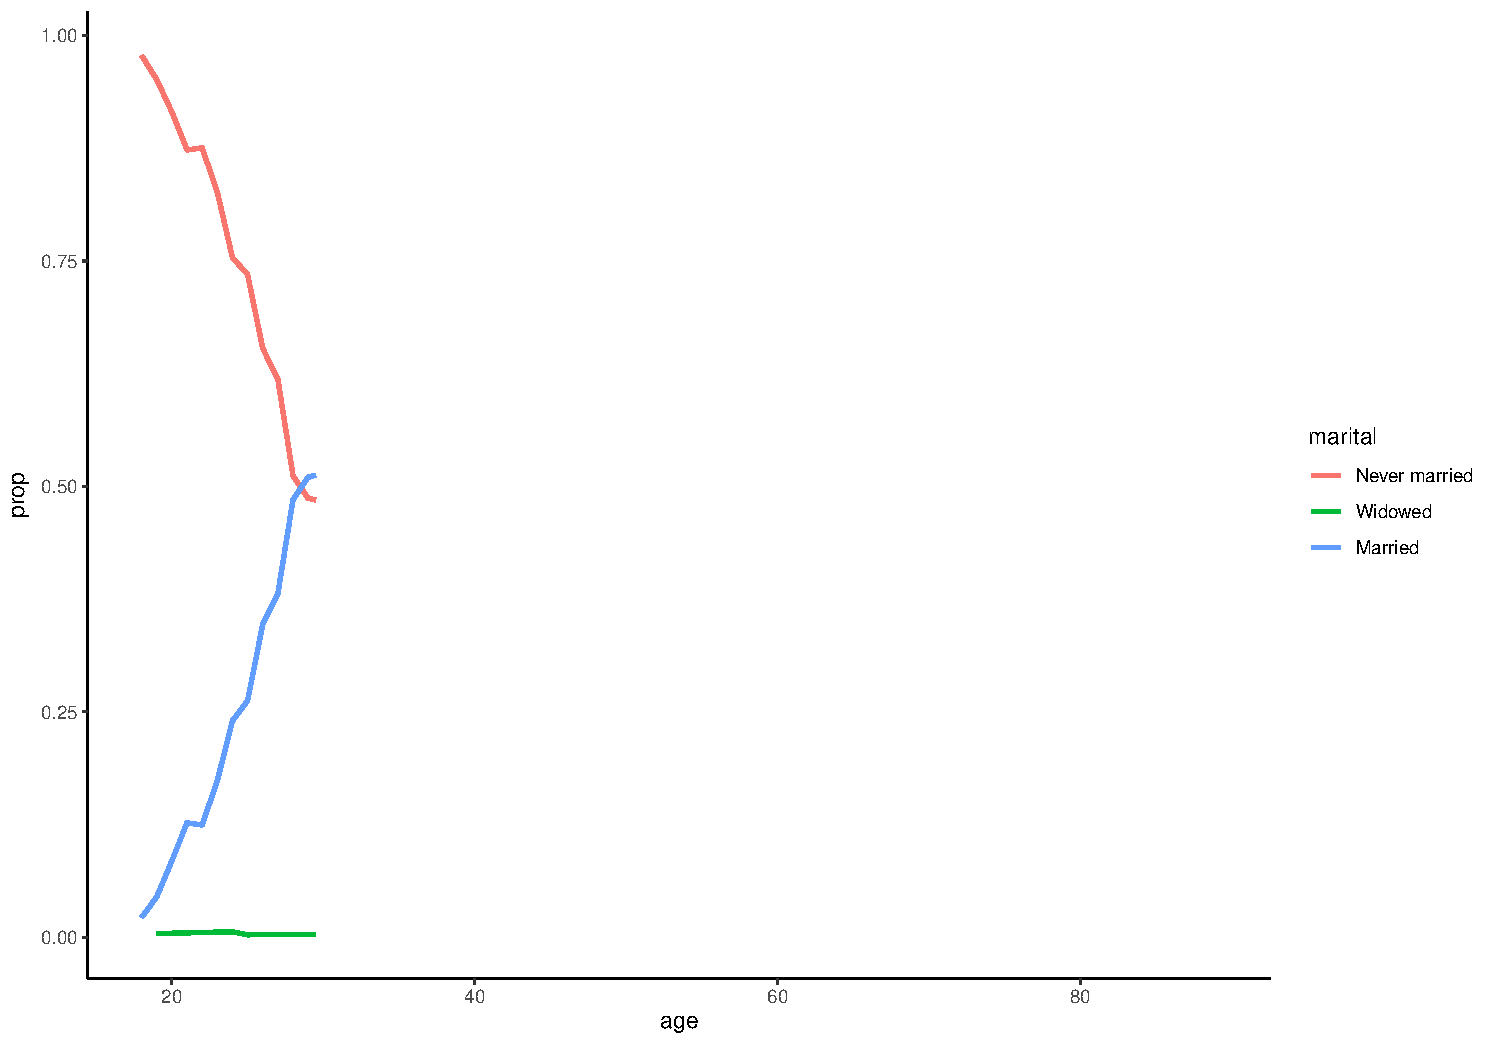
\includegraphics{gss_cat_files/figure-beamer/unnamed-chunk-1-21.pdf}

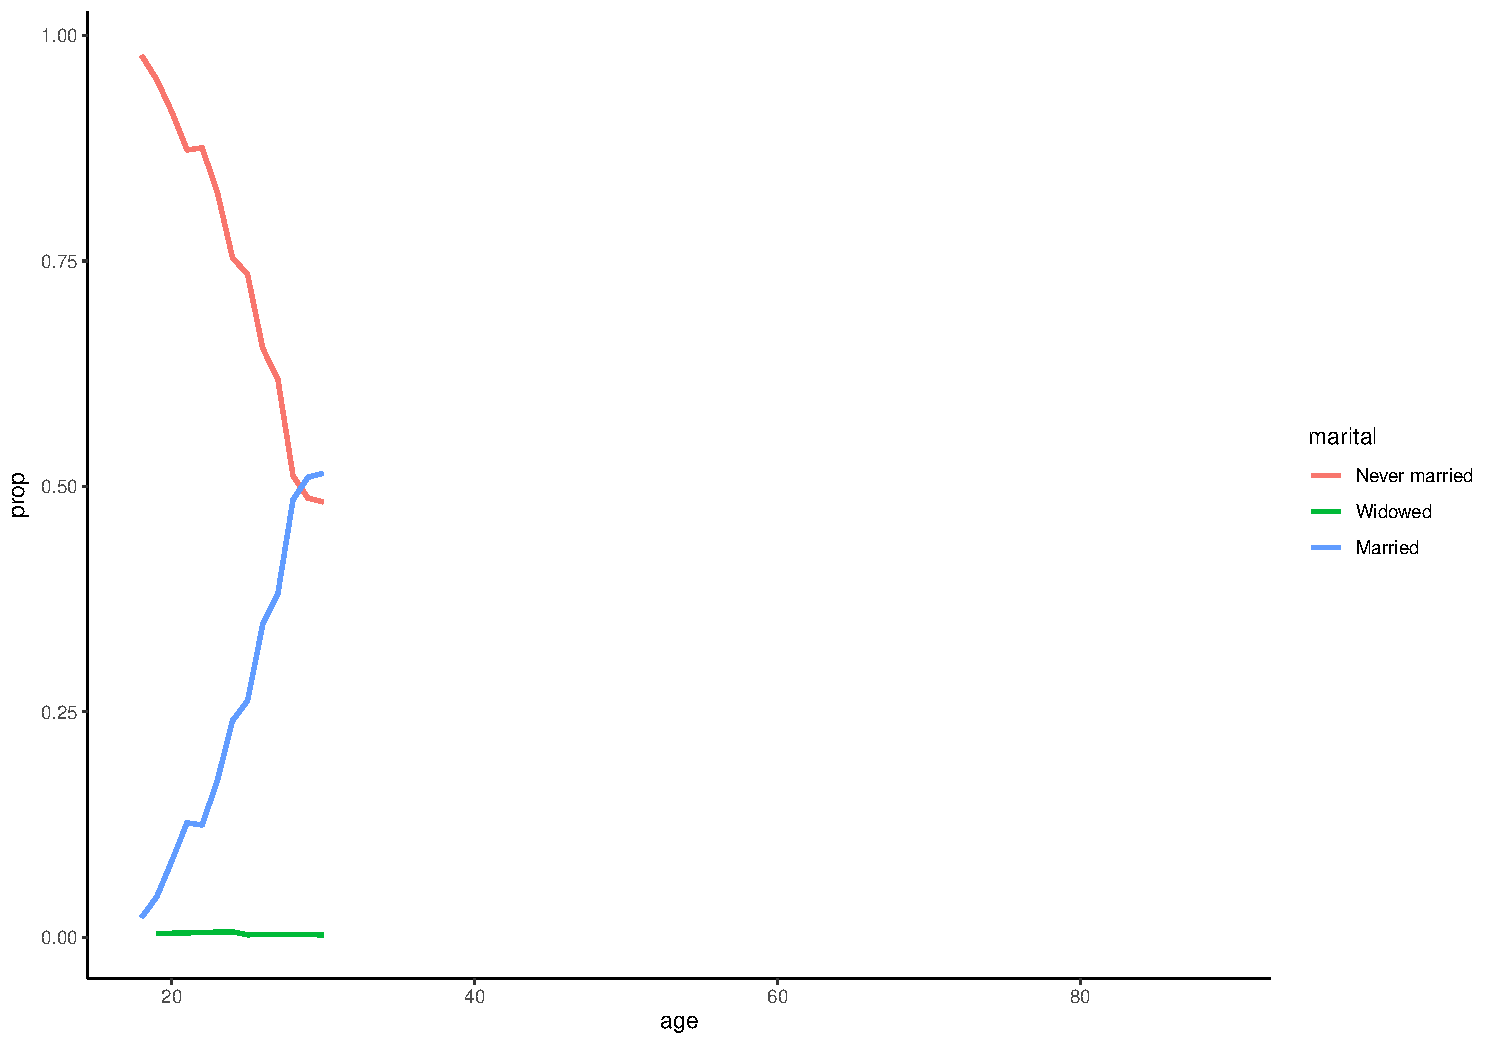
\includegraphics{gss_cat_files/figure-beamer/unnamed-chunk-1-22.pdf}

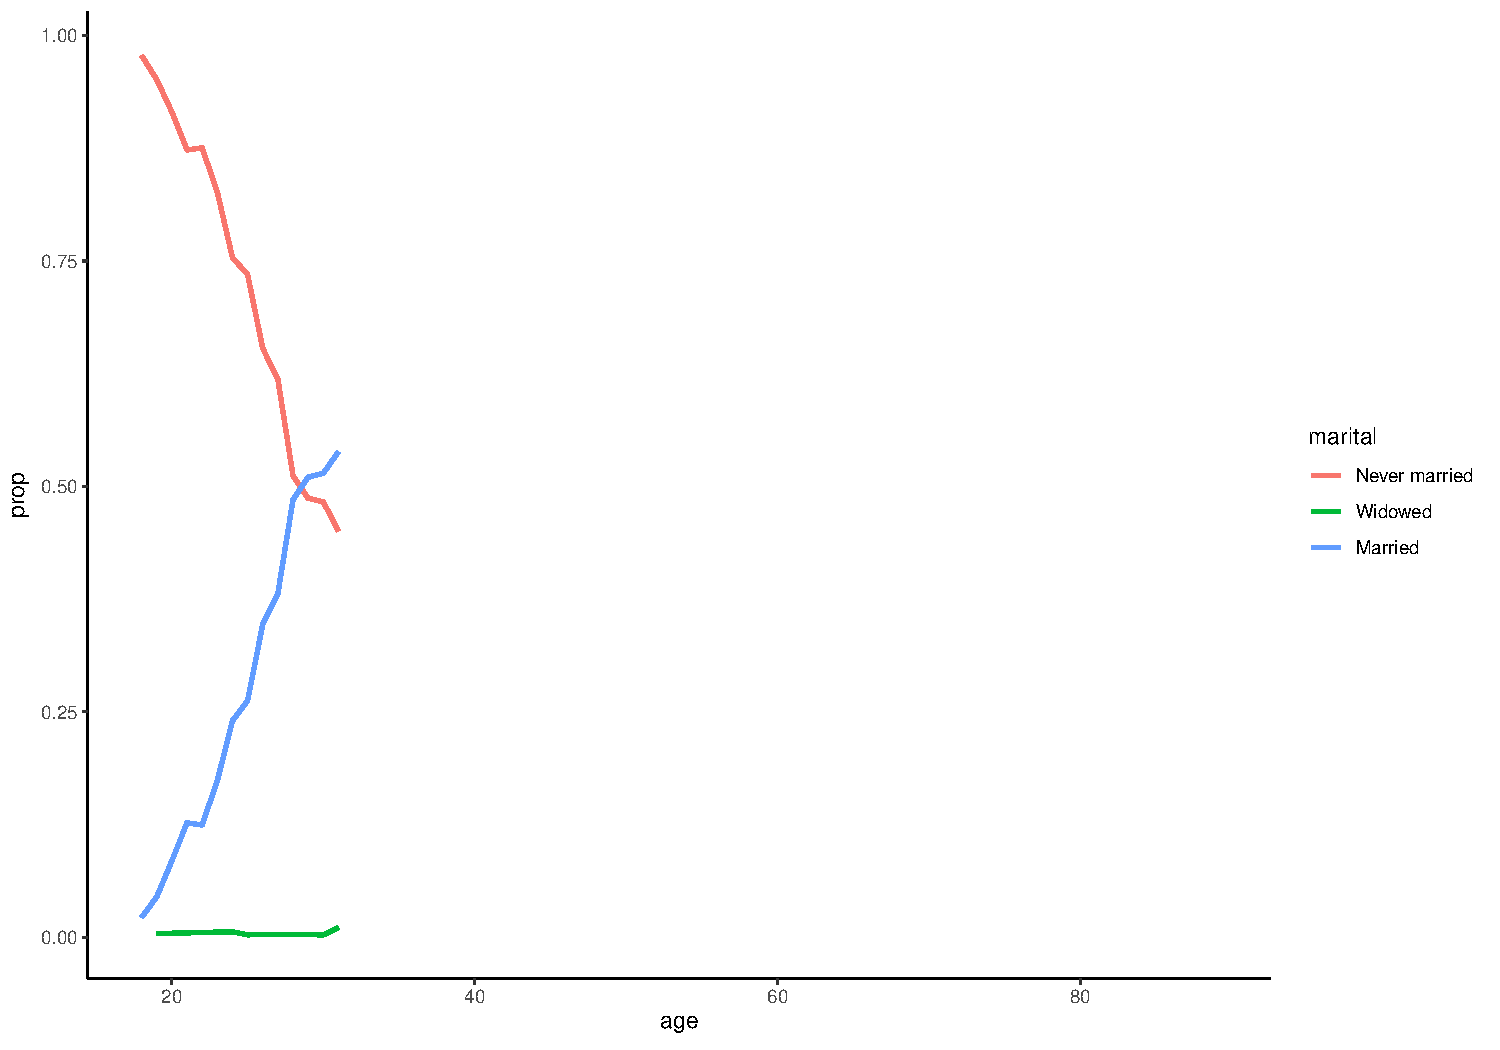
\includegraphics{gss_cat_files/figure-beamer/unnamed-chunk-1-23.pdf}

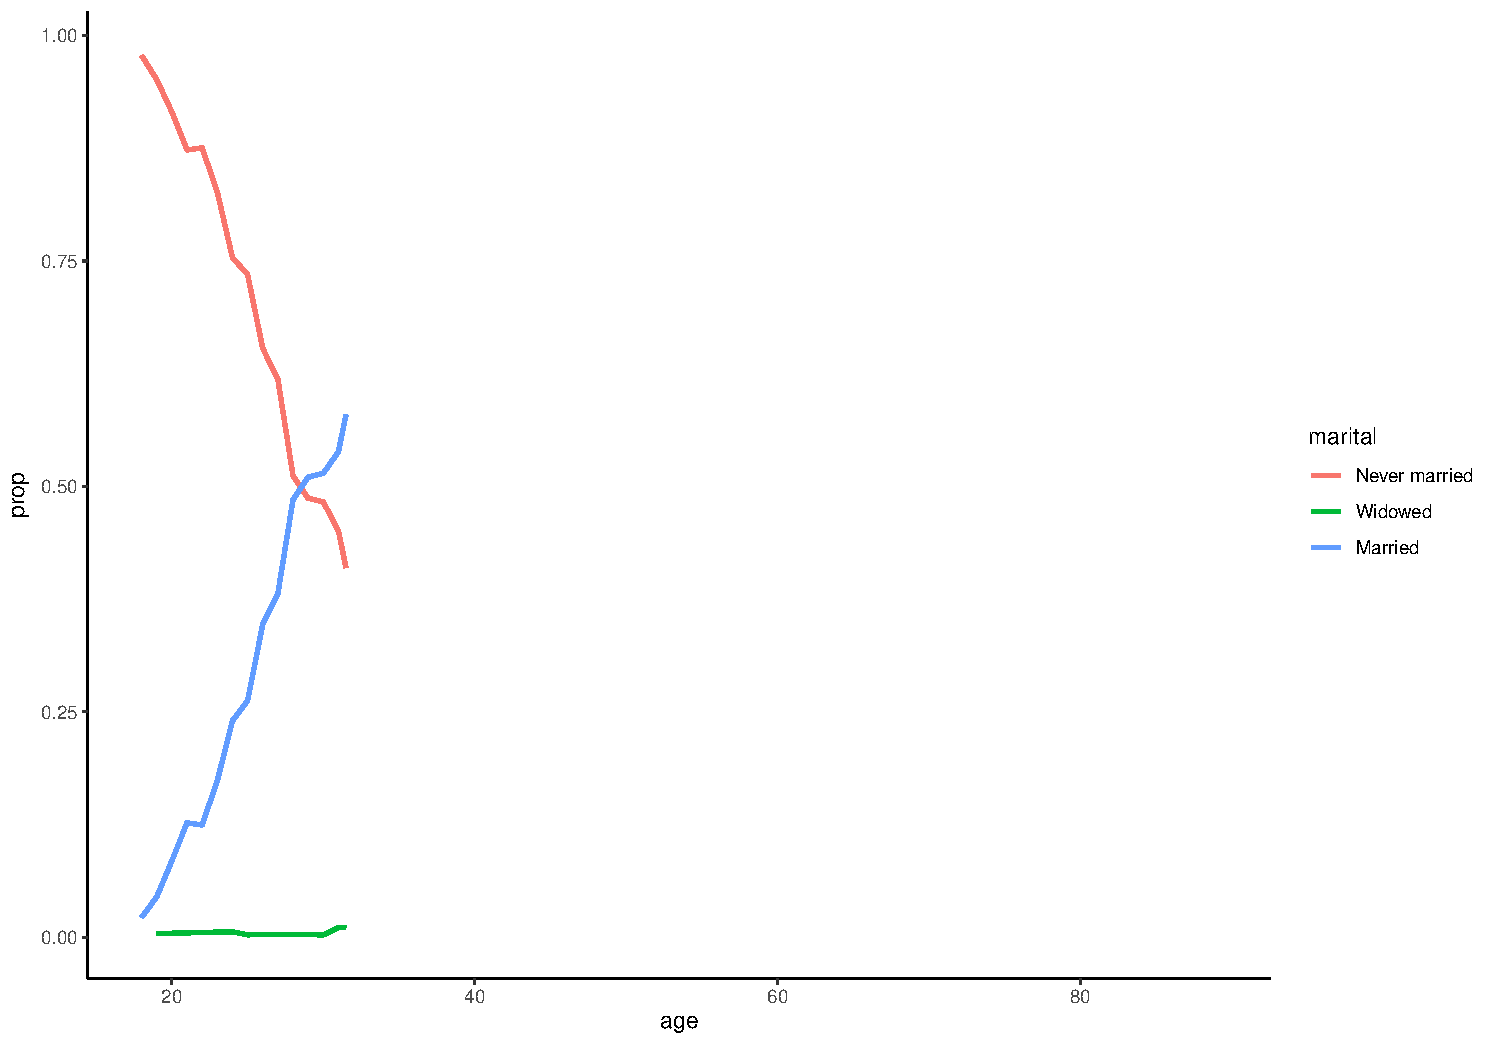
\includegraphics{gss_cat_files/figure-beamer/unnamed-chunk-1-24.pdf}

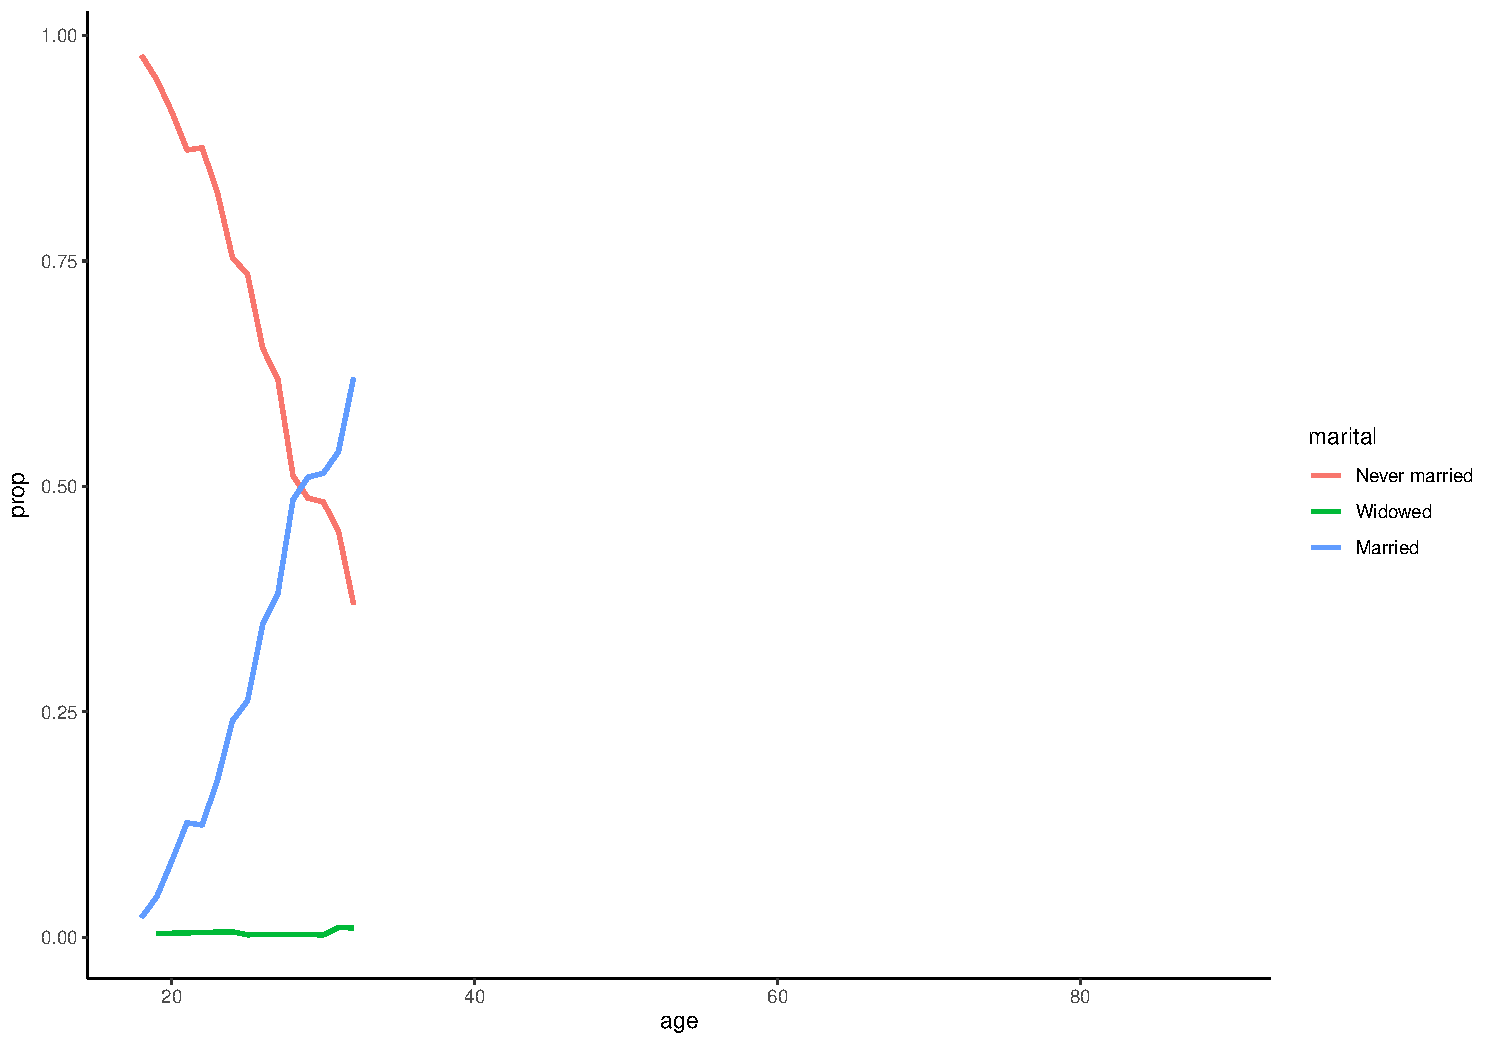
\includegraphics{gss_cat_files/figure-beamer/unnamed-chunk-1-25.pdf}

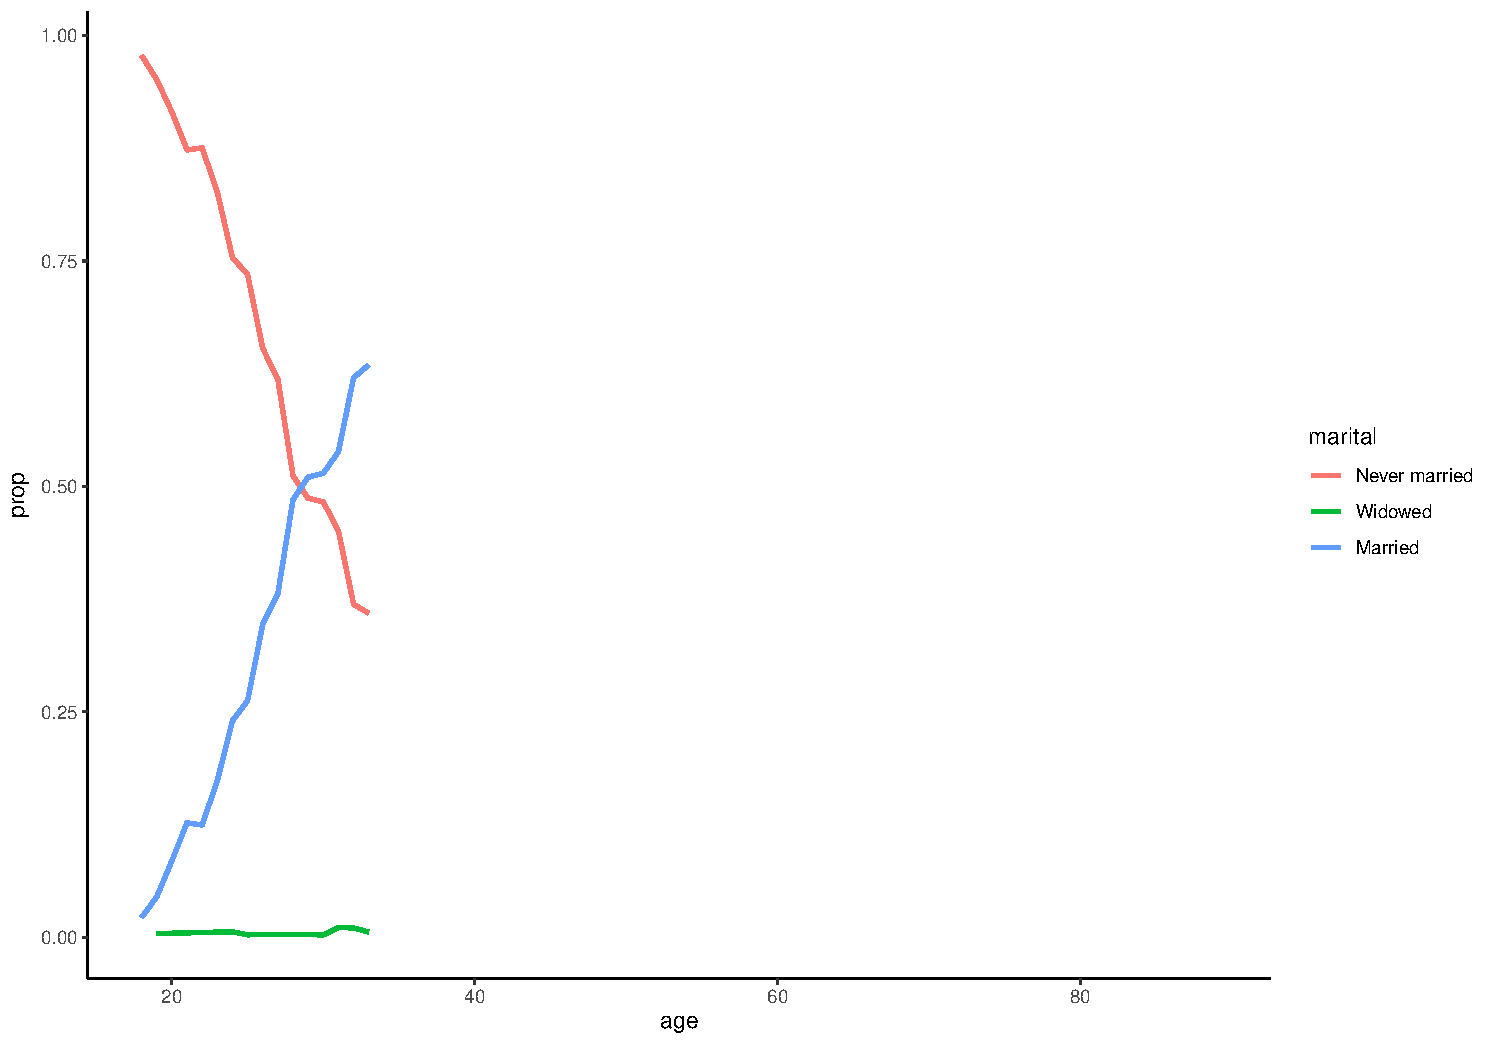
\includegraphics{gss_cat_files/figure-beamer/unnamed-chunk-1-26.pdf}

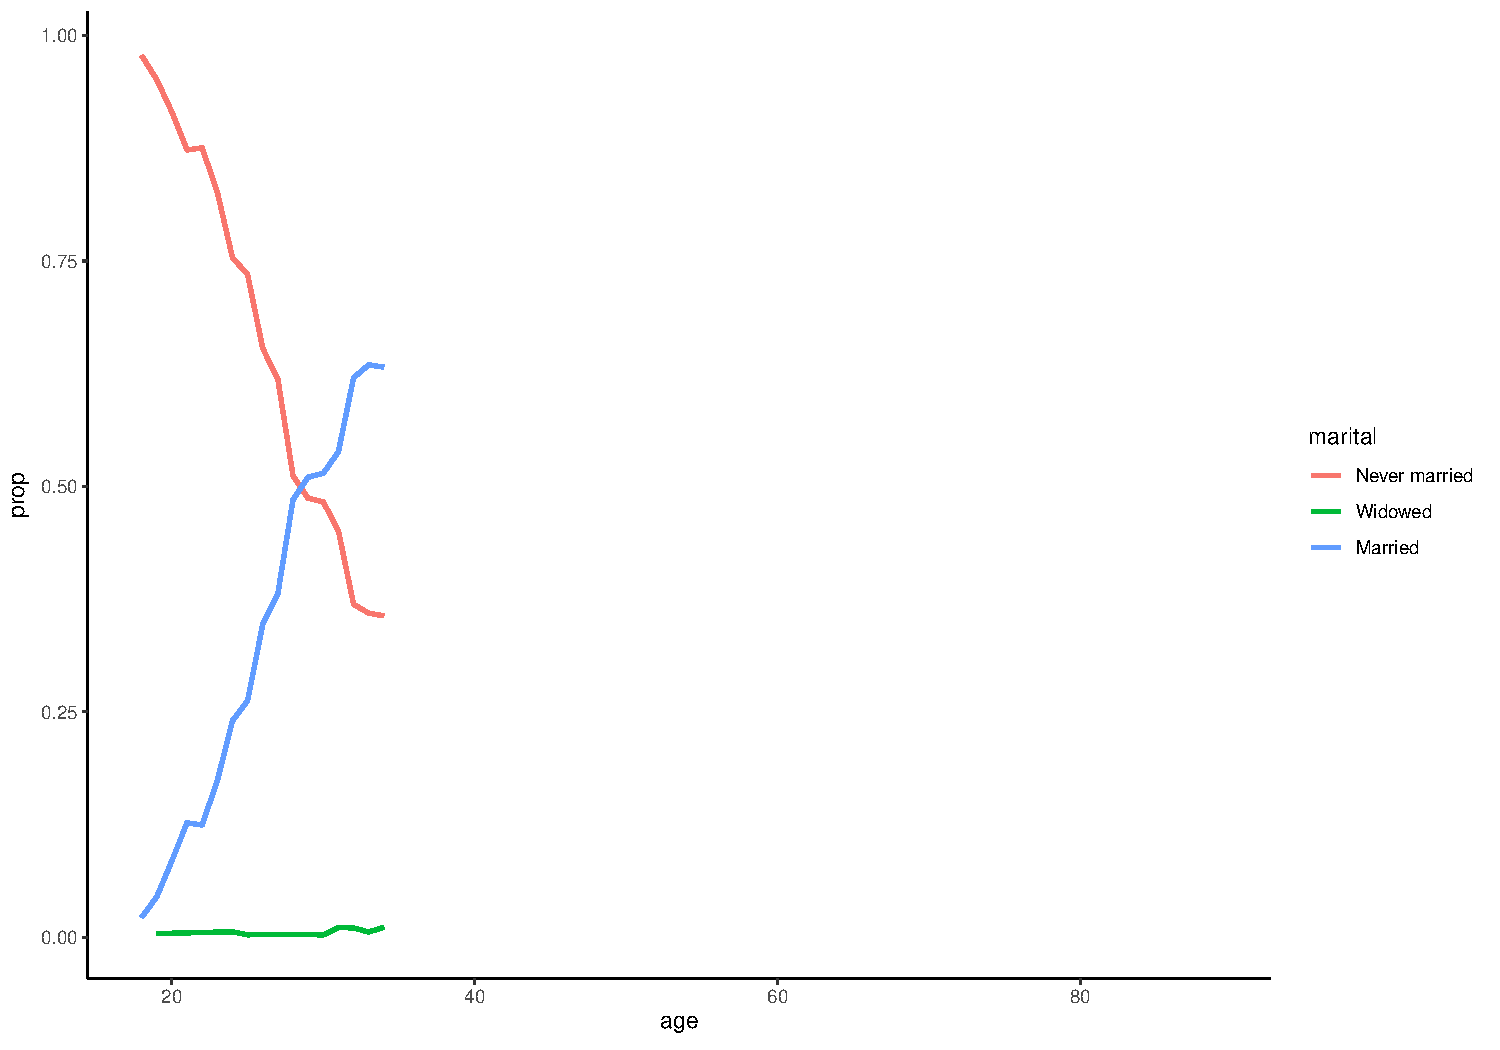
\includegraphics{gss_cat_files/figure-beamer/unnamed-chunk-1-27.pdf}

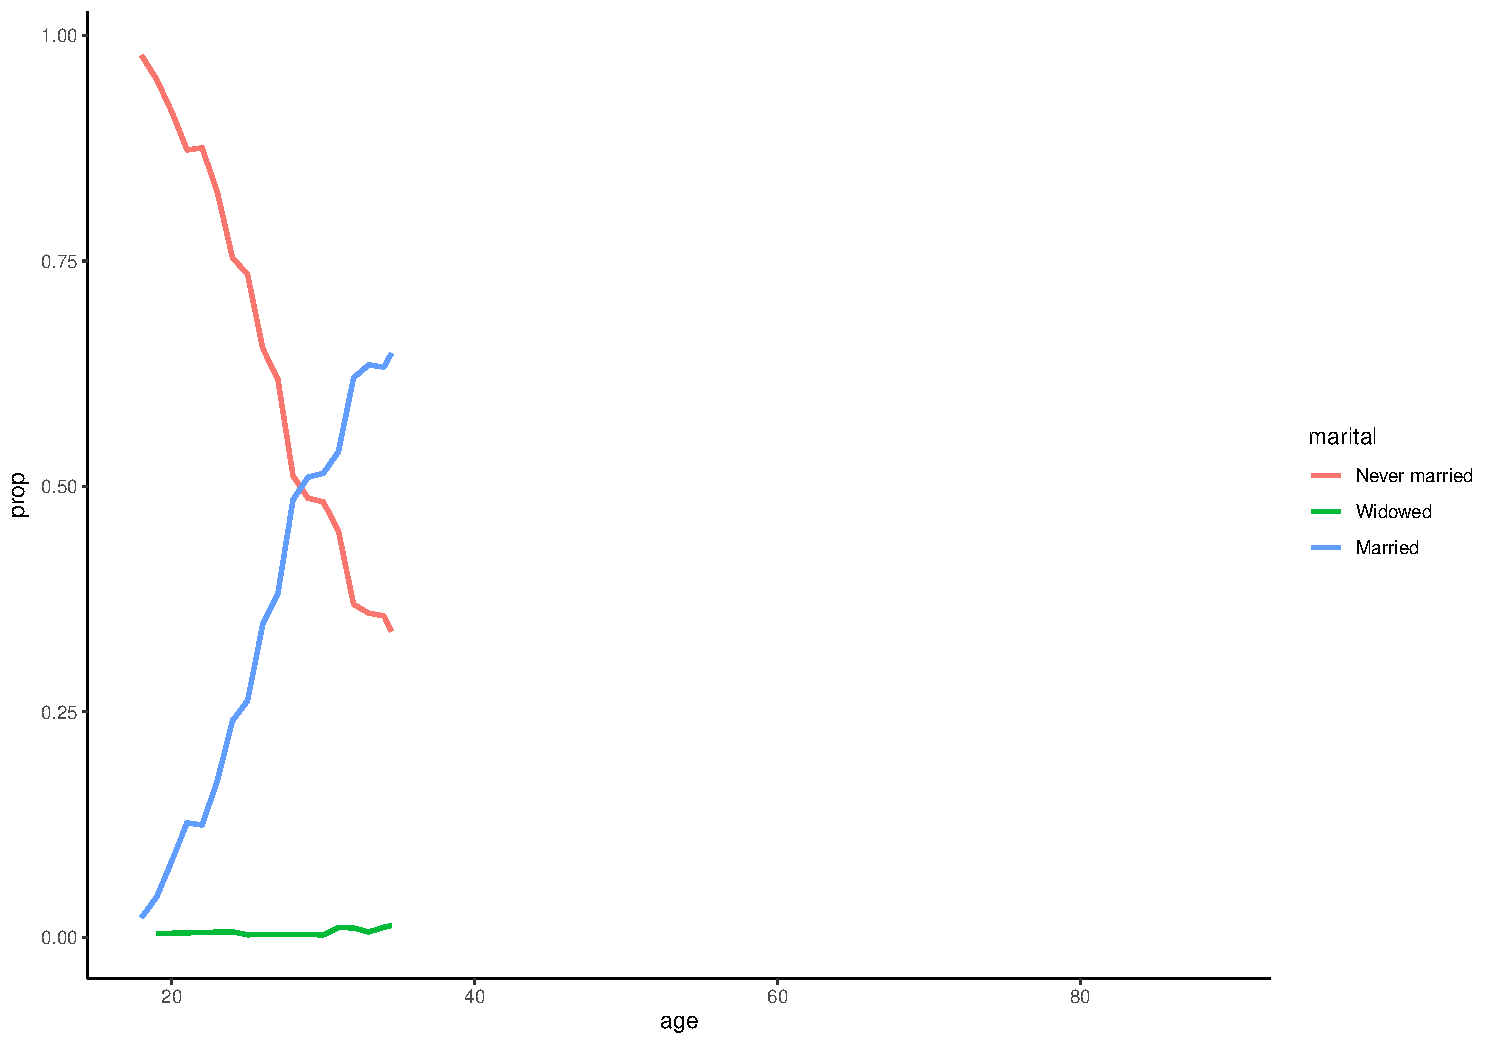
\includegraphics{gss_cat_files/figure-beamer/unnamed-chunk-1-28.pdf}

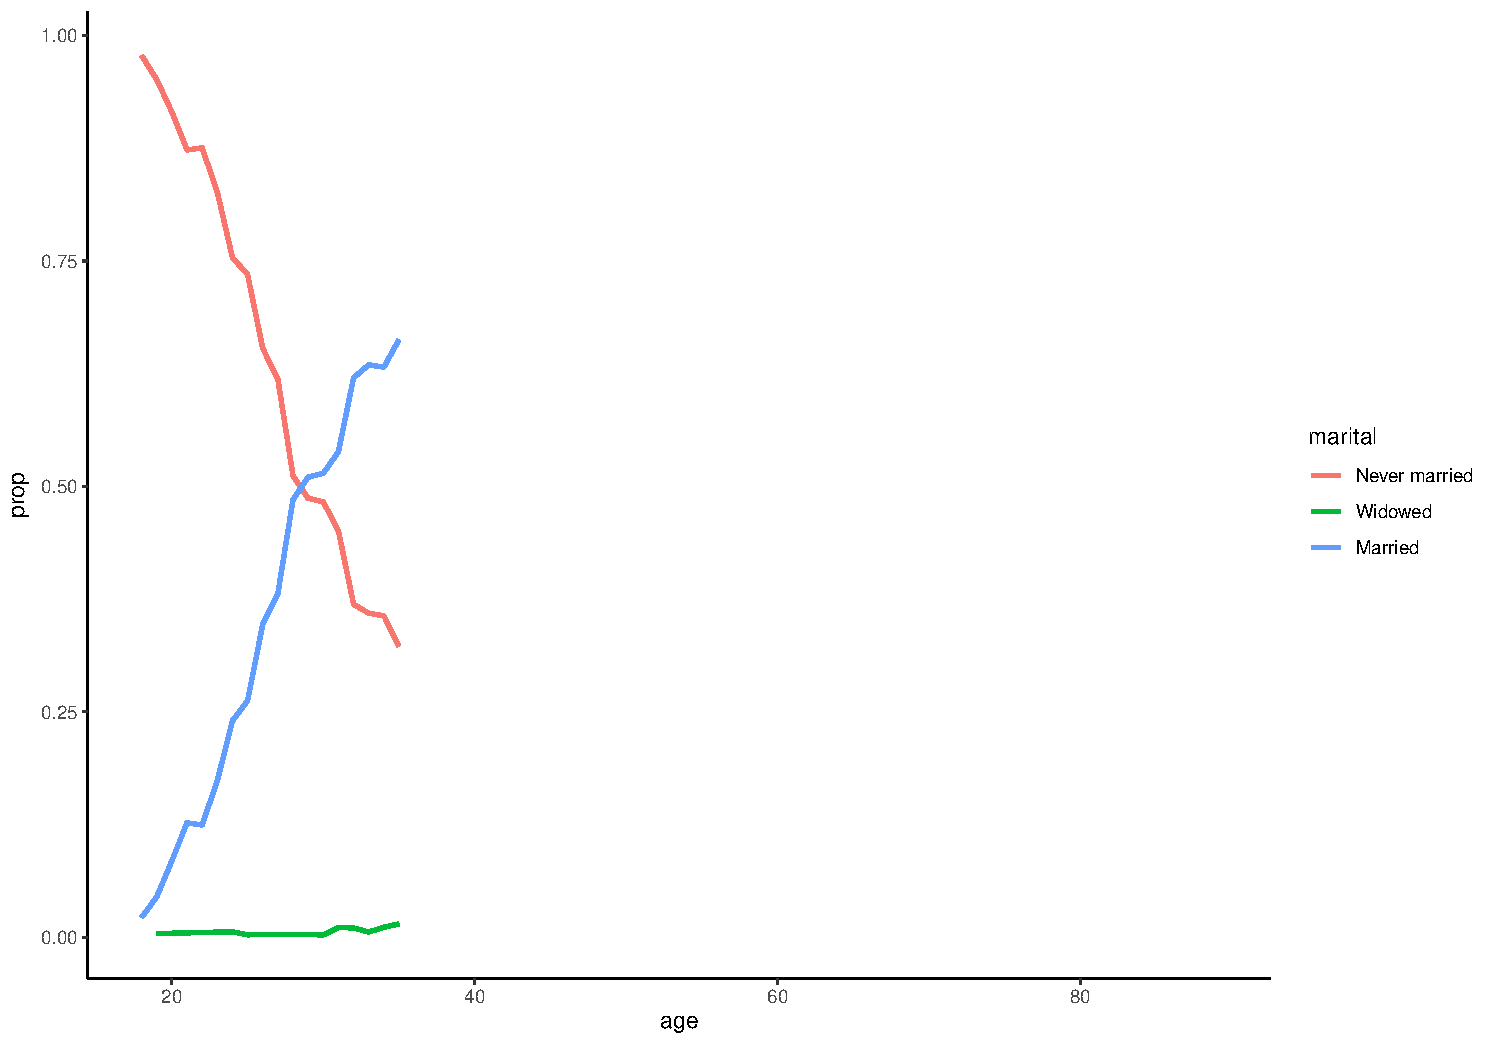
\includegraphics{gss_cat_files/figure-beamer/unnamed-chunk-1-29.pdf}

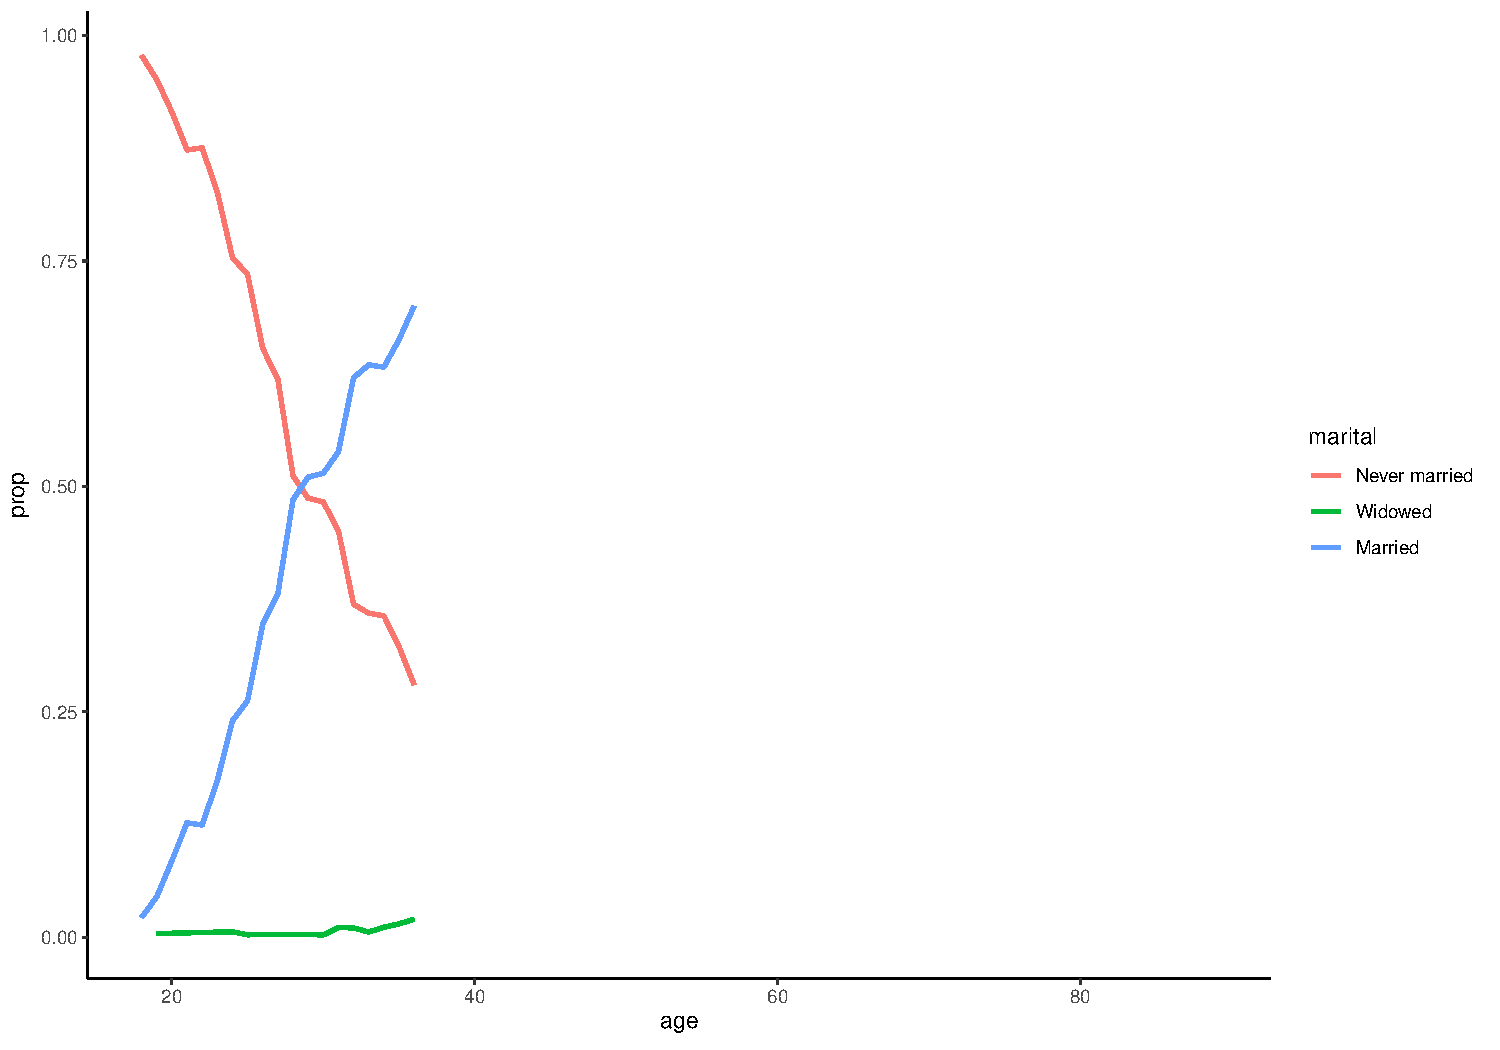
\includegraphics{gss_cat_files/figure-beamer/unnamed-chunk-1-30.pdf}

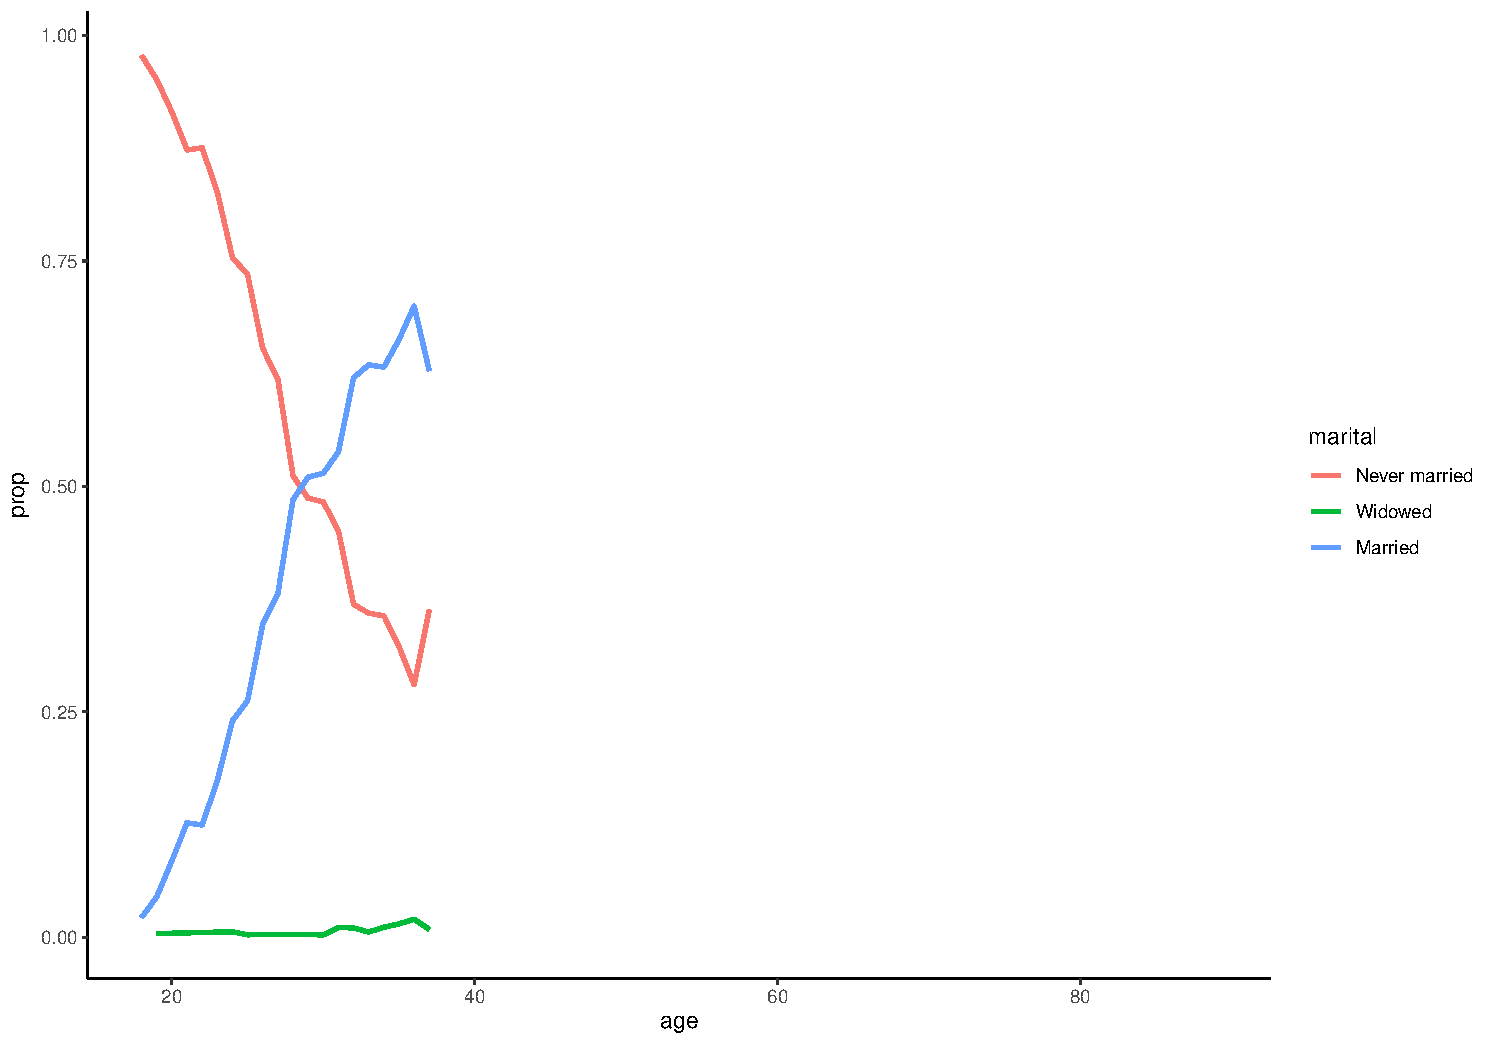
\includegraphics{gss_cat_files/figure-beamer/unnamed-chunk-1-31.pdf}

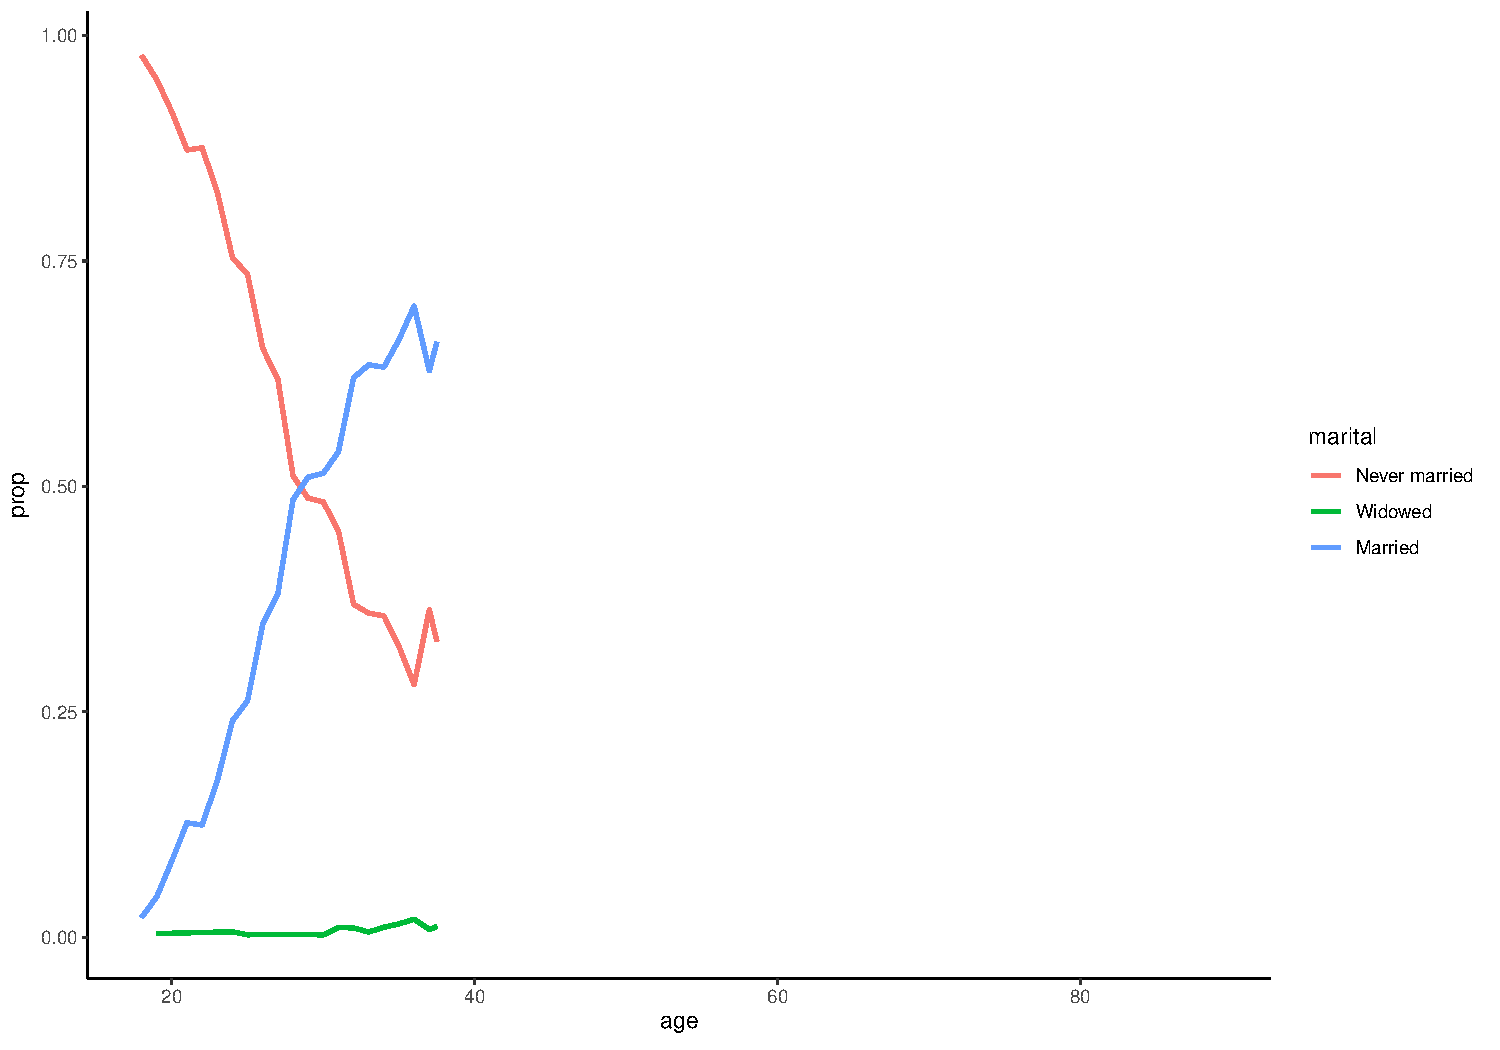
\includegraphics{gss_cat_files/figure-beamer/unnamed-chunk-1-32.pdf}

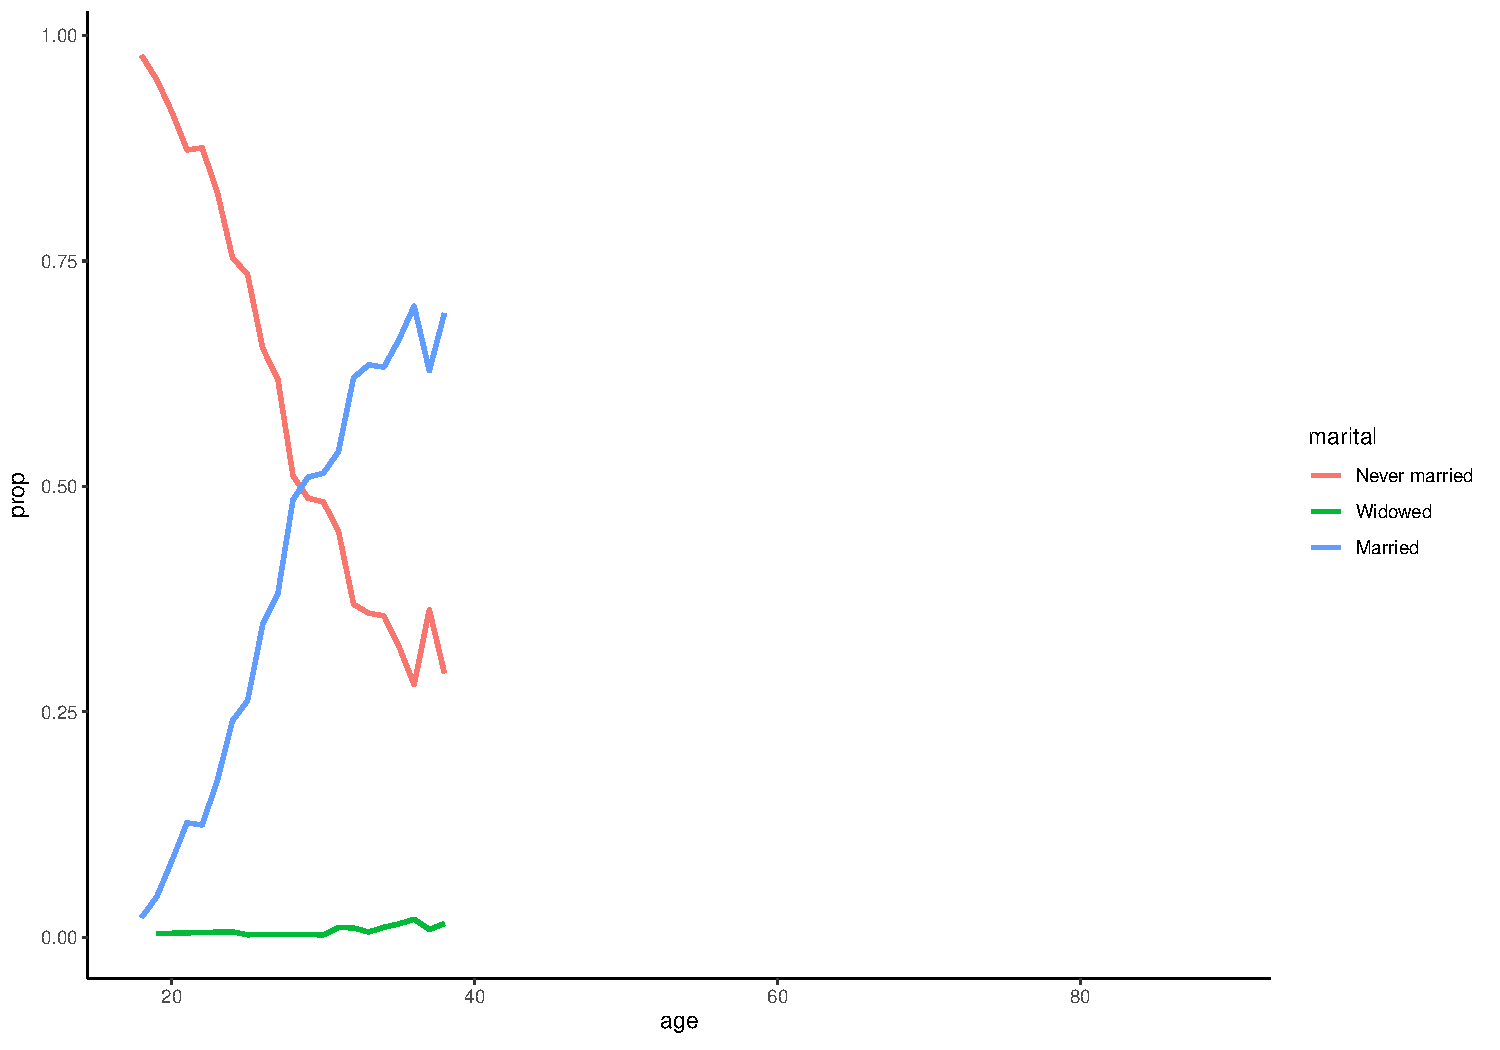
\includegraphics{gss_cat_files/figure-beamer/unnamed-chunk-1-33.pdf}

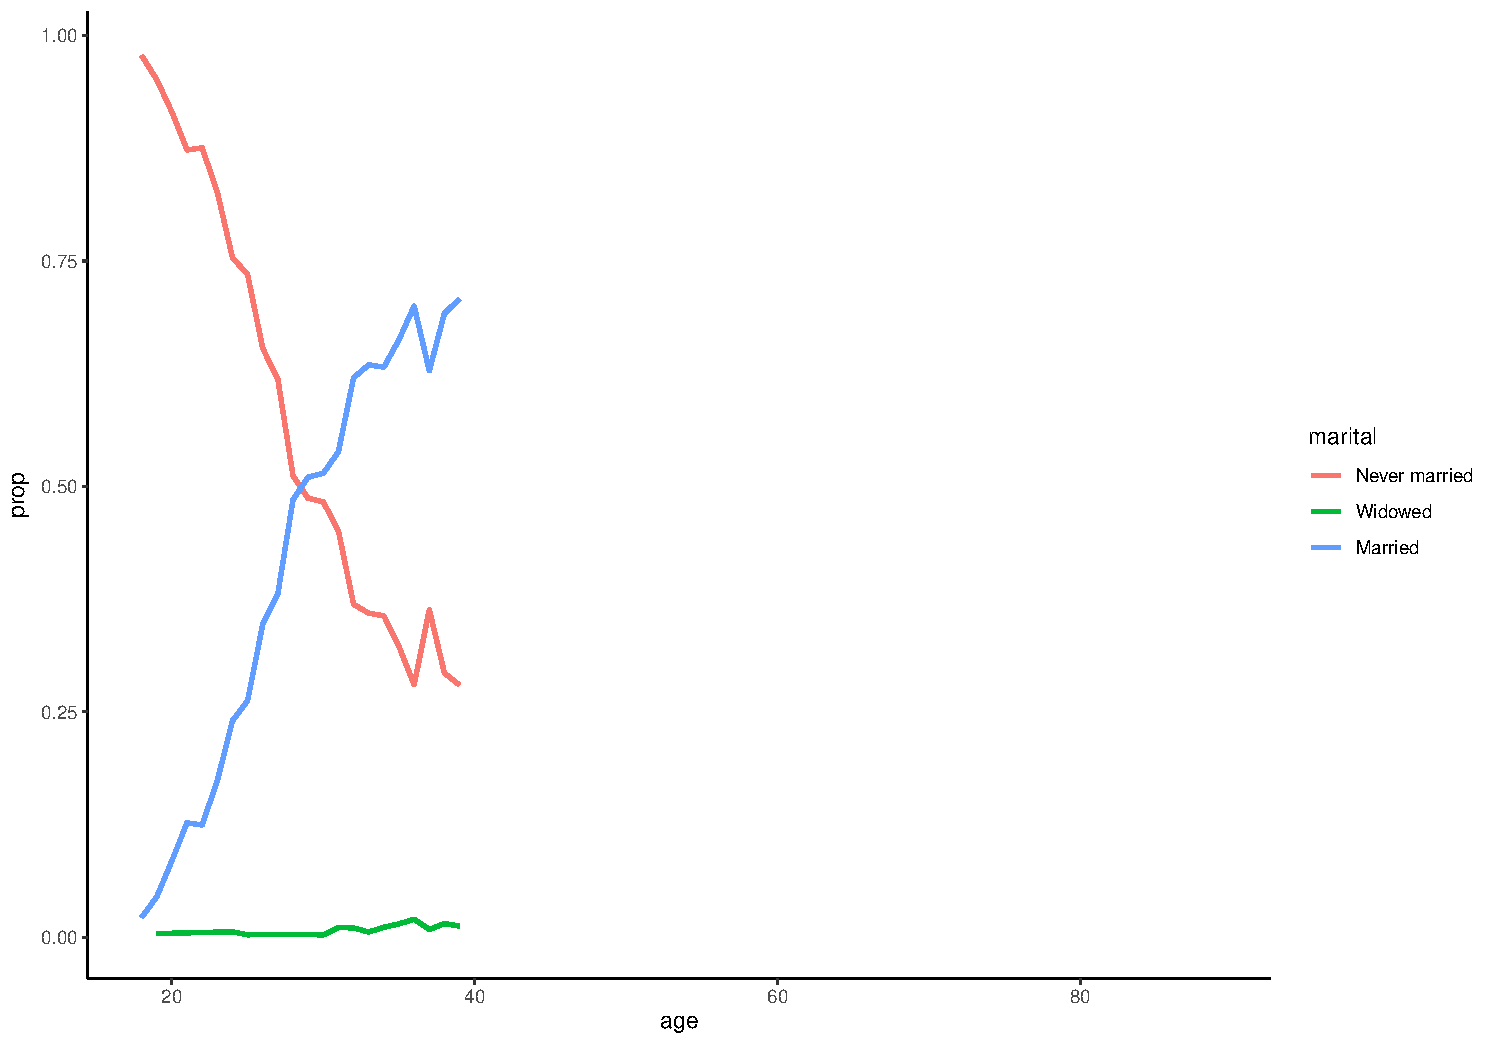
\includegraphics{gss_cat_files/figure-beamer/unnamed-chunk-1-34.pdf}

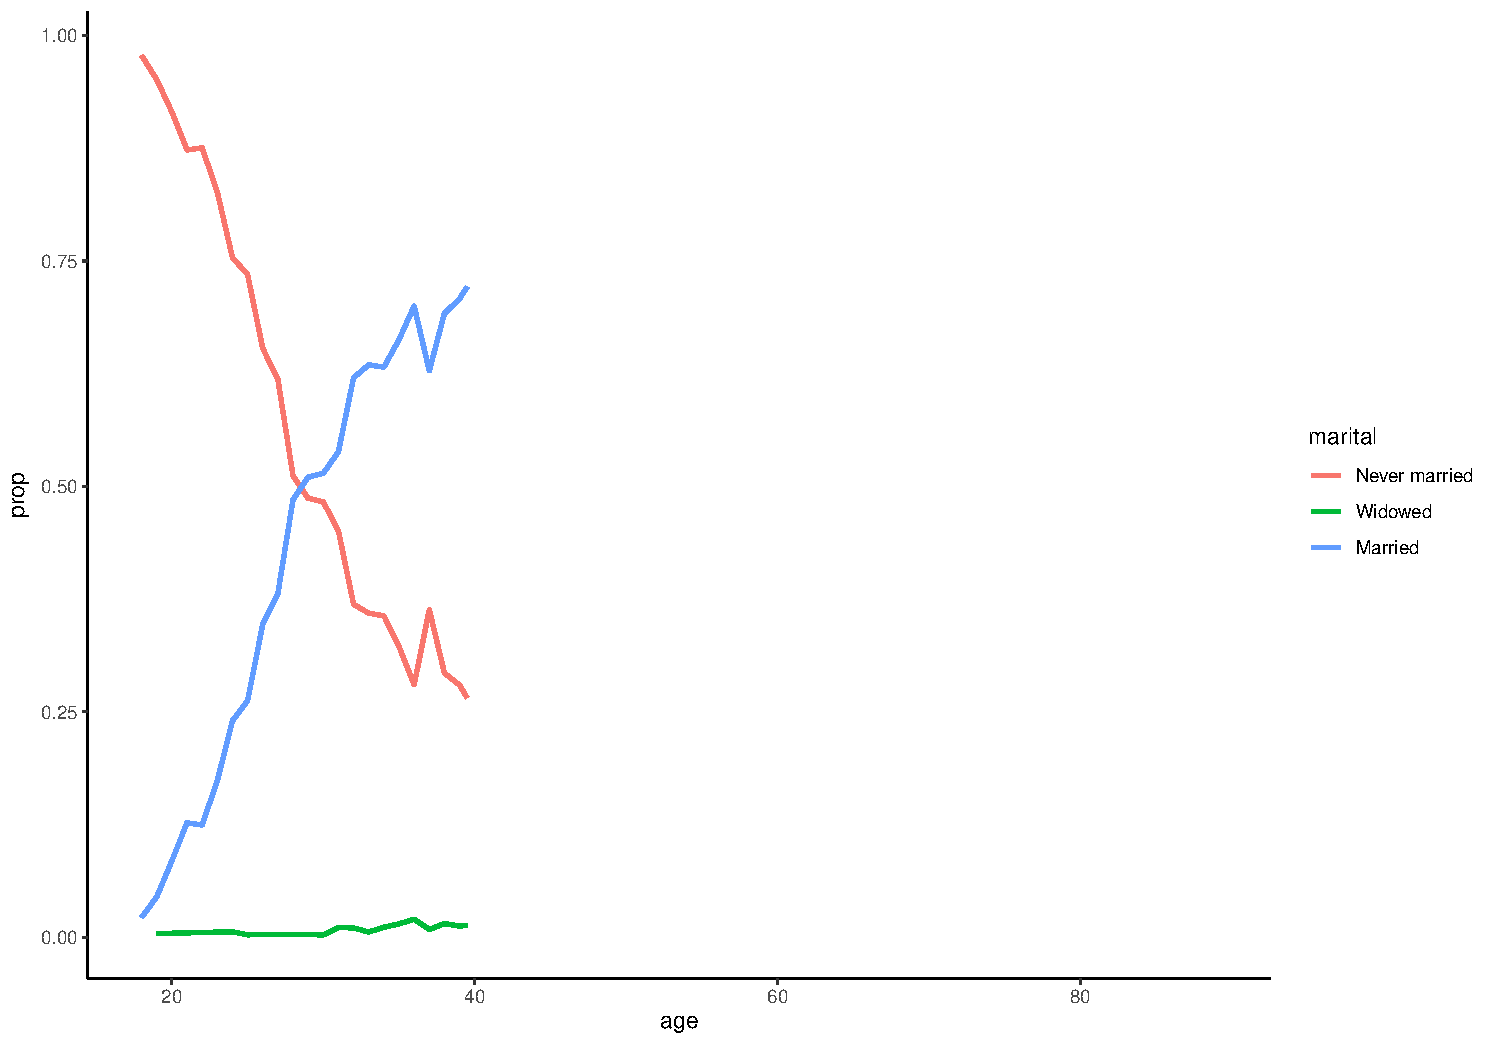
\includegraphics{gss_cat_files/figure-beamer/unnamed-chunk-1-35.pdf}

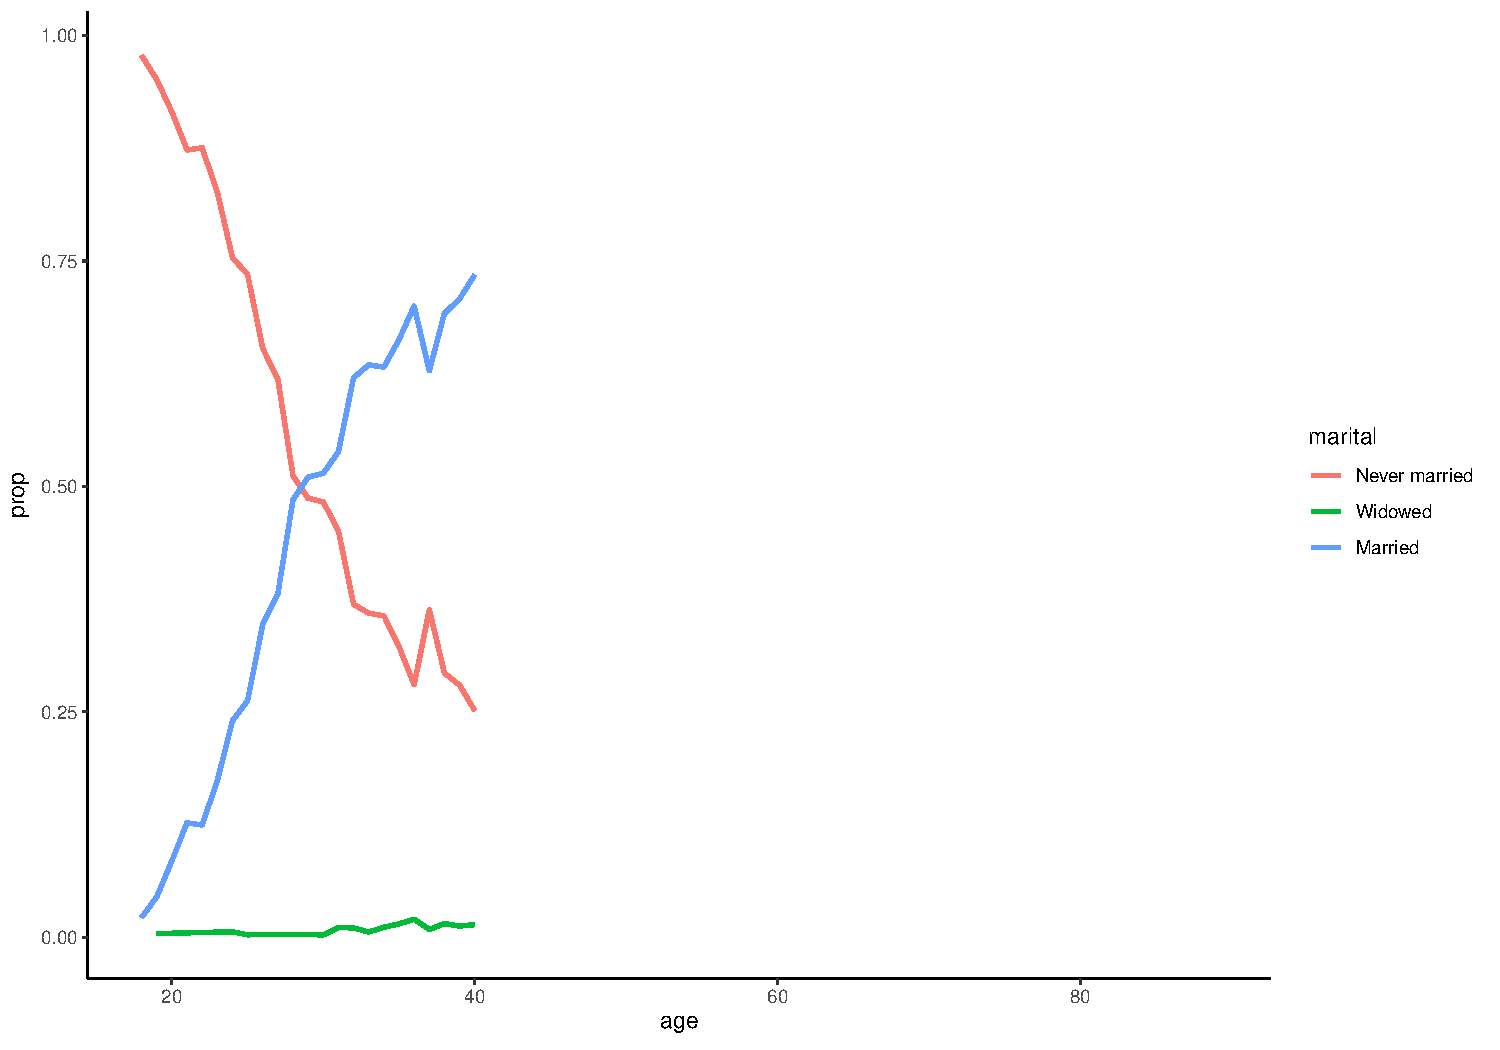
\includegraphics{gss_cat_files/figure-beamer/unnamed-chunk-1-36.pdf}

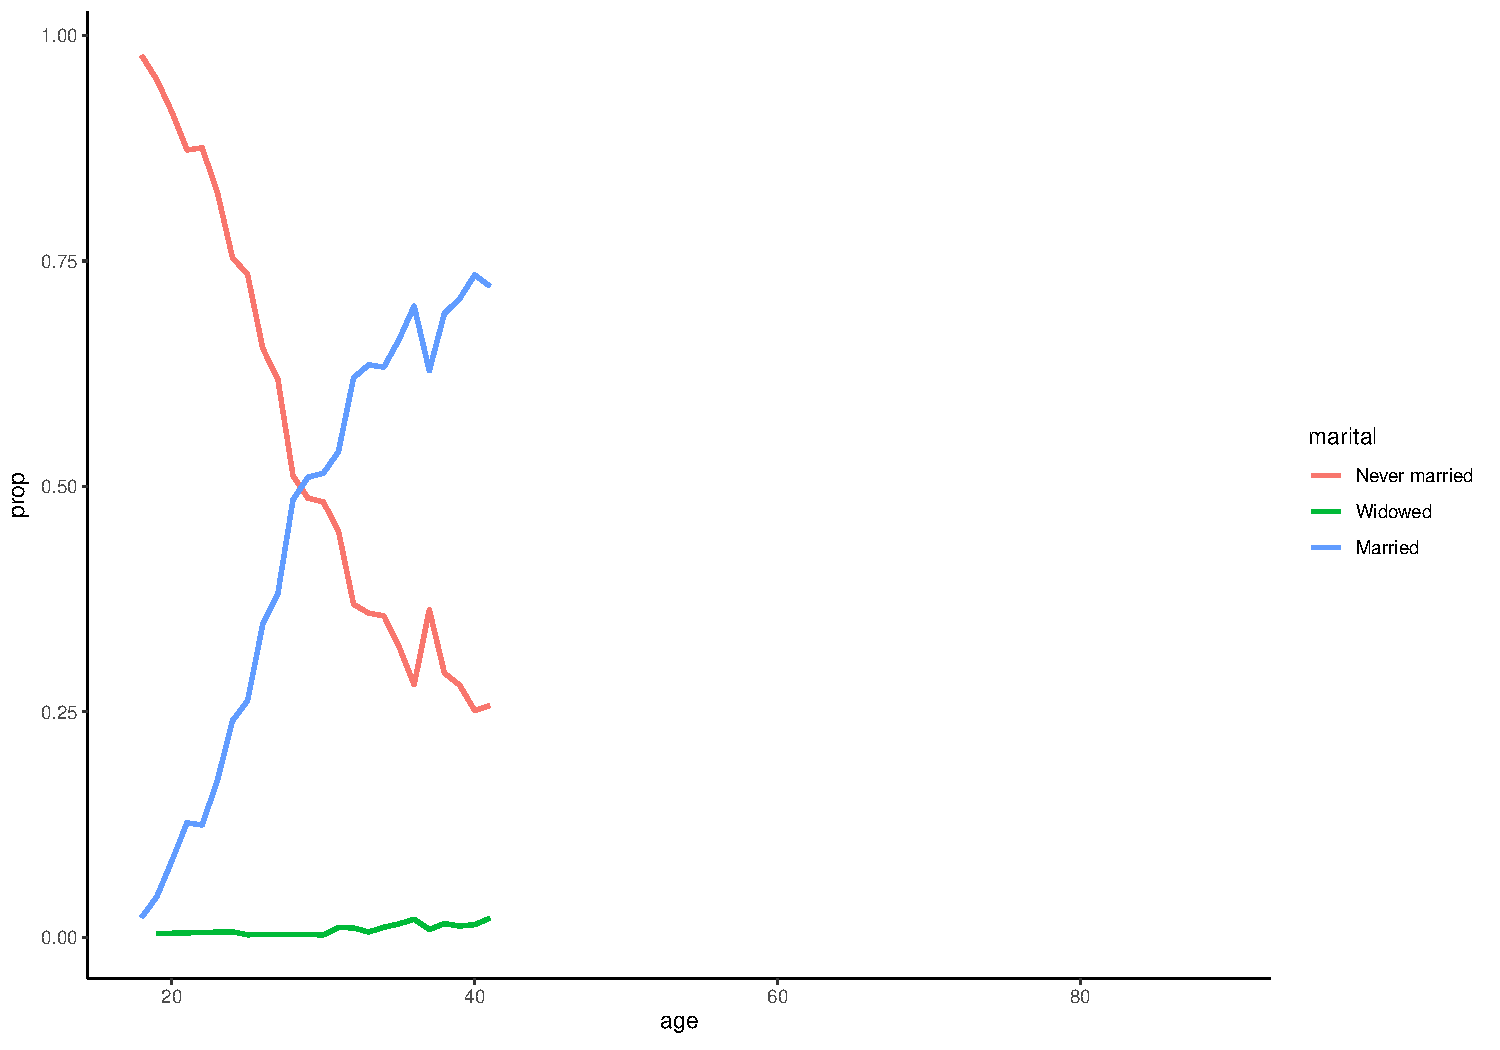
\includegraphics{gss_cat_files/figure-beamer/unnamed-chunk-1-37.pdf}

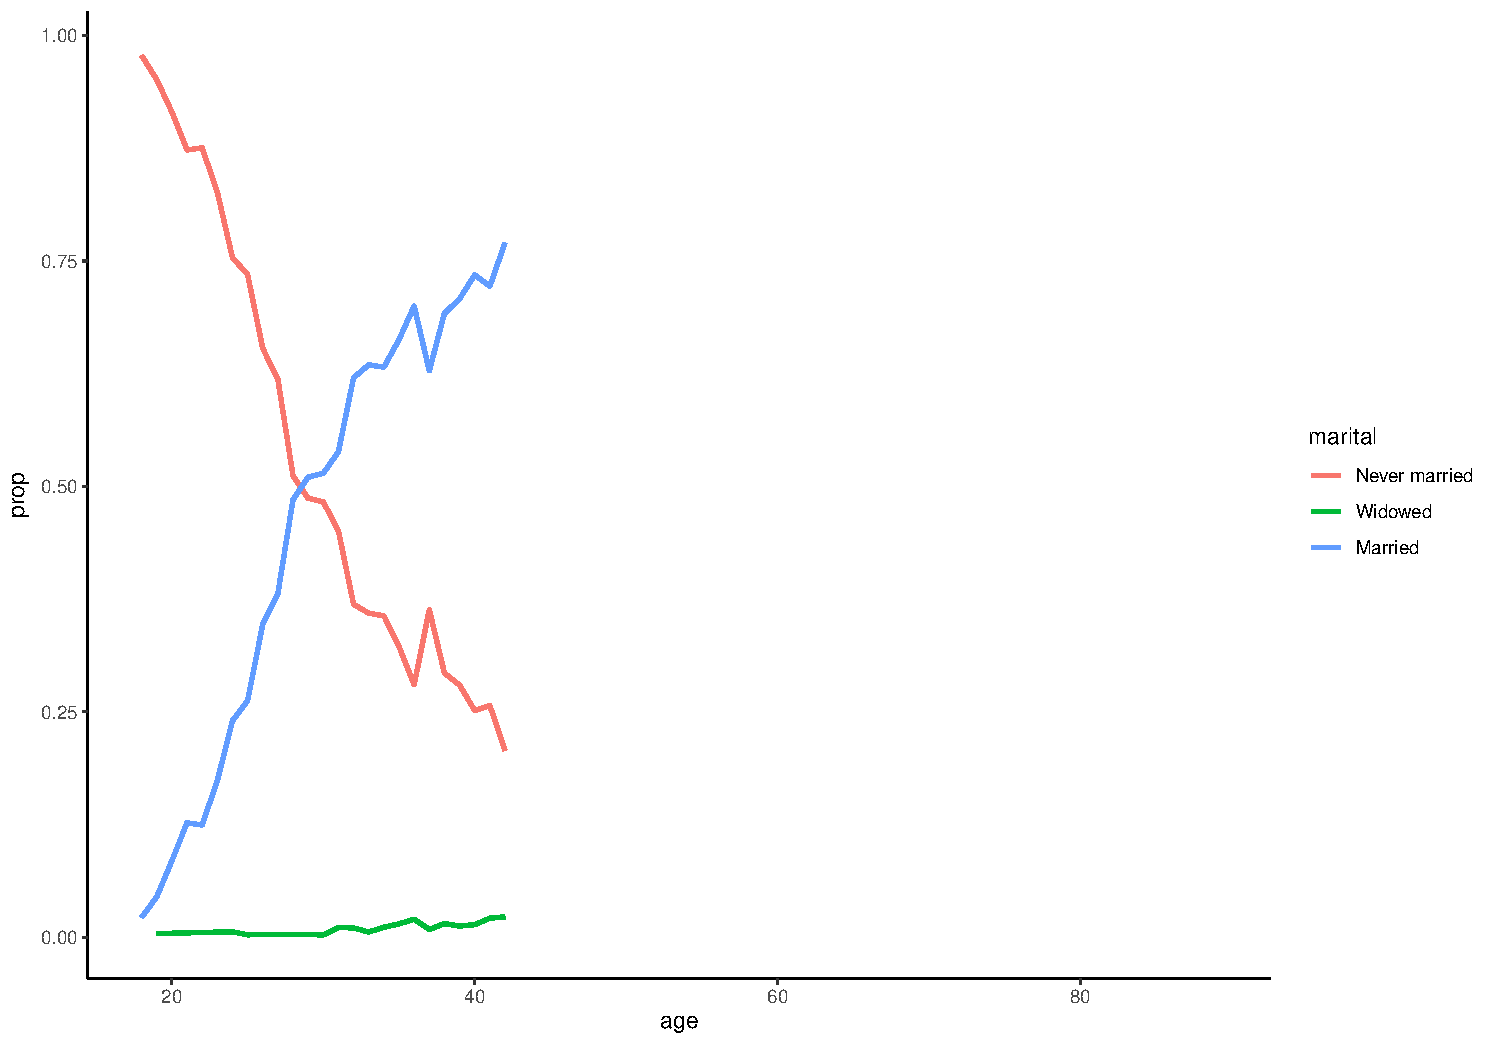
\includegraphics{gss_cat_files/figure-beamer/unnamed-chunk-1-38.pdf}

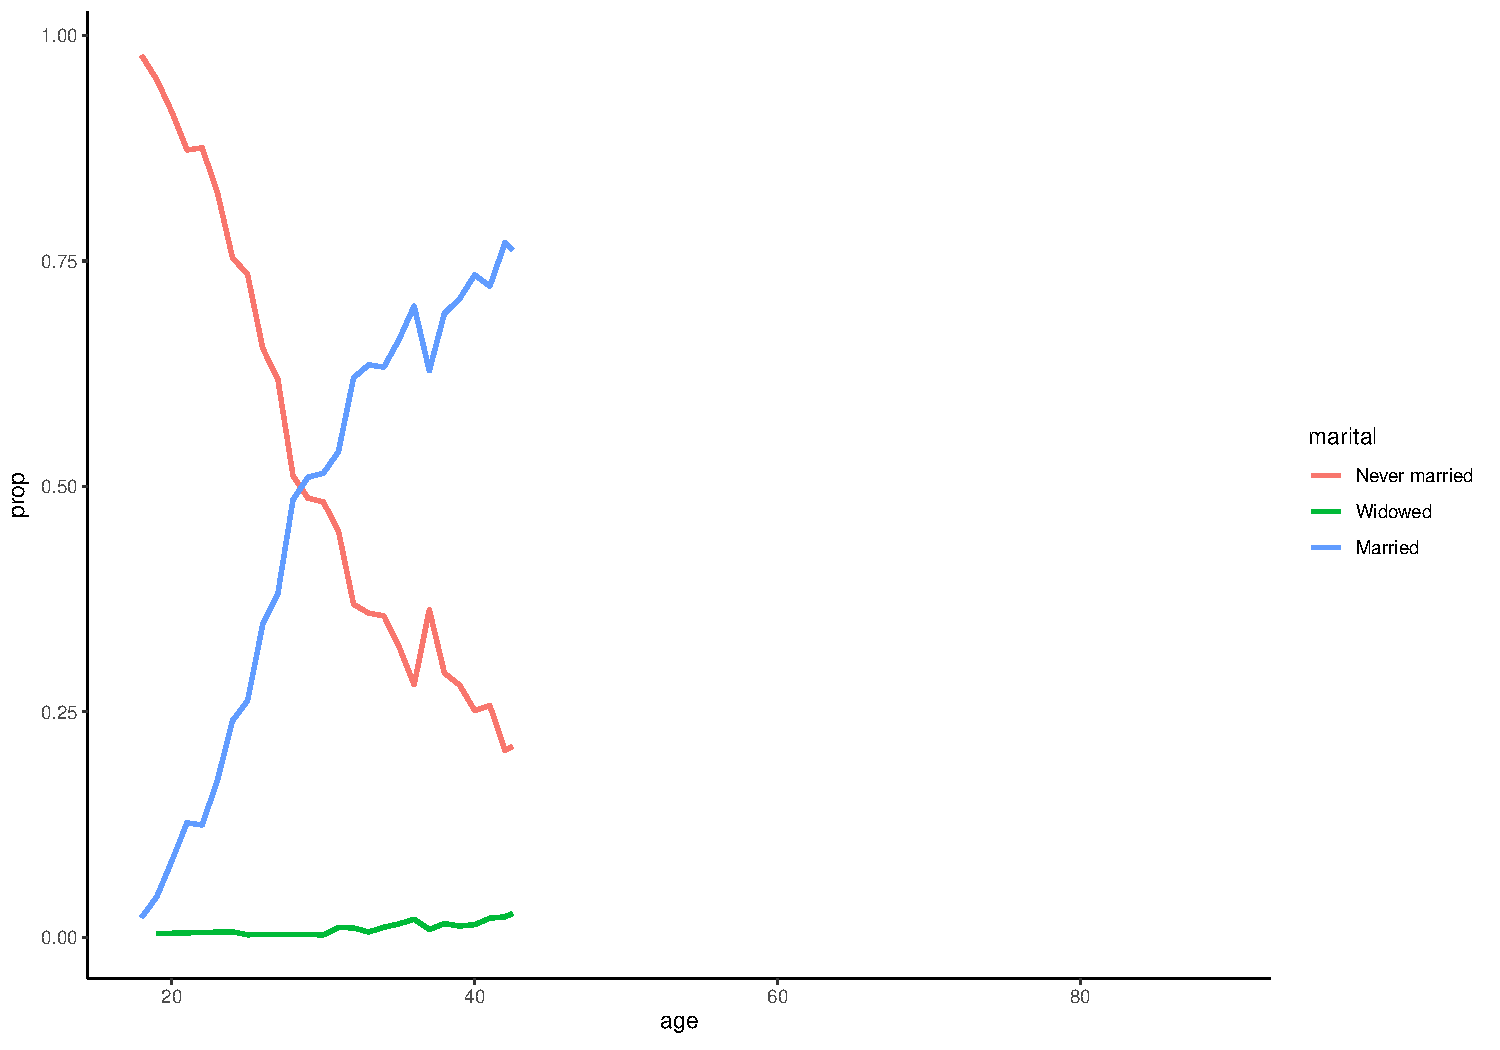
\includegraphics{gss_cat_files/figure-beamer/unnamed-chunk-1-39.pdf}

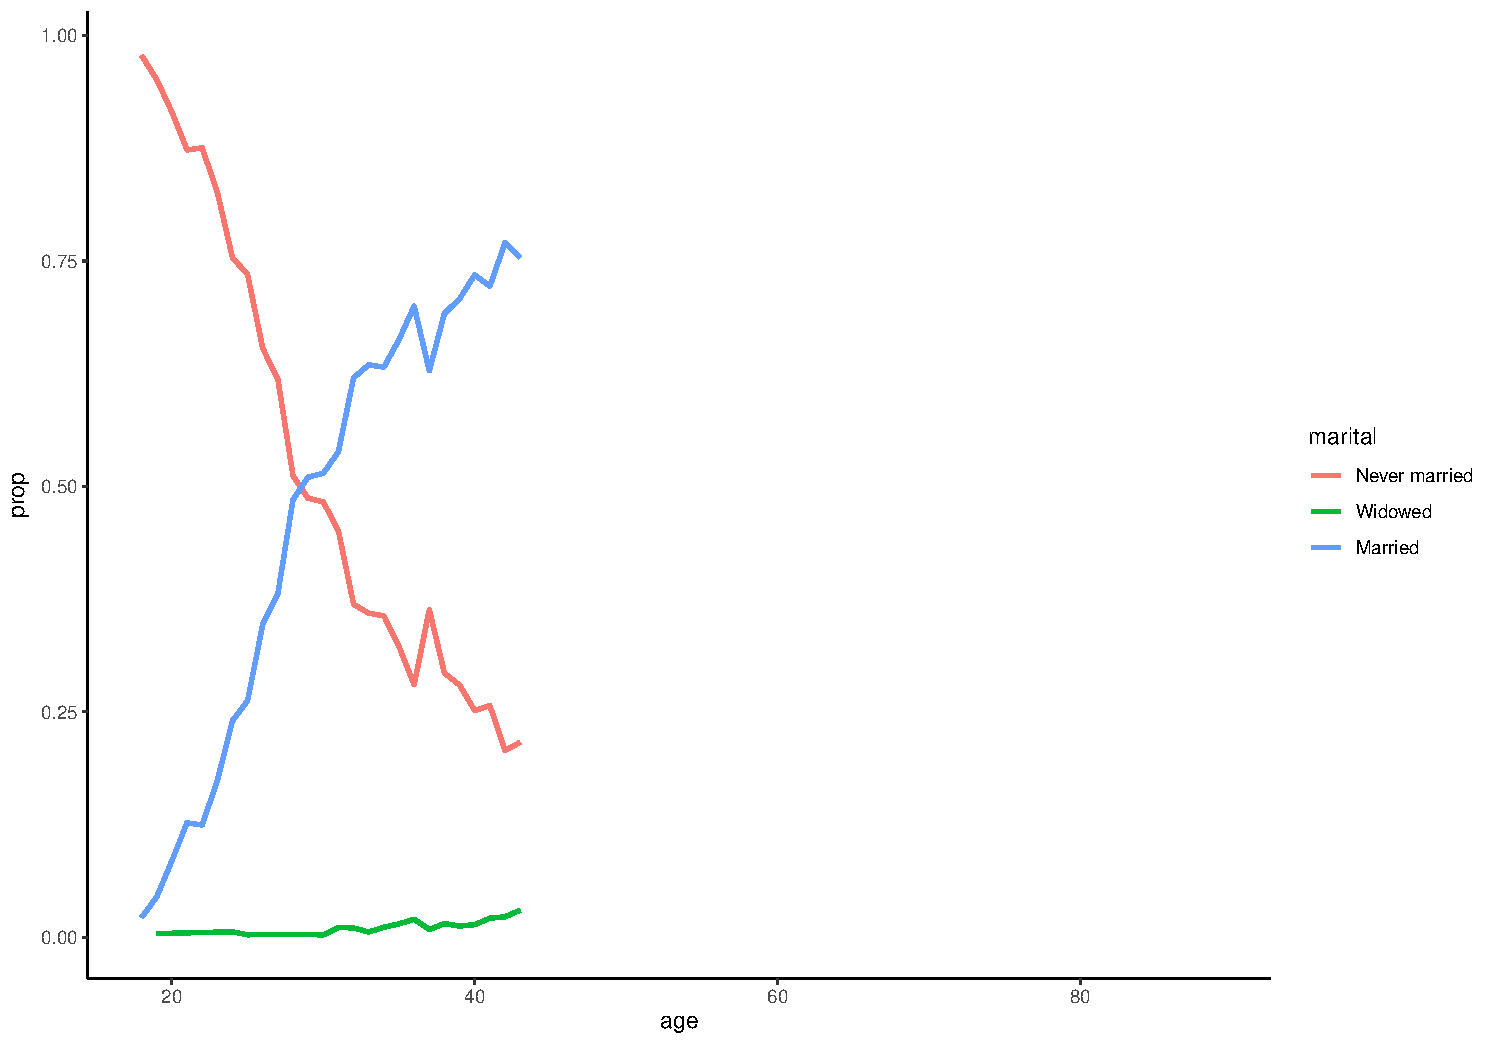
\includegraphics{gss_cat_files/figure-beamer/unnamed-chunk-1-40.pdf}

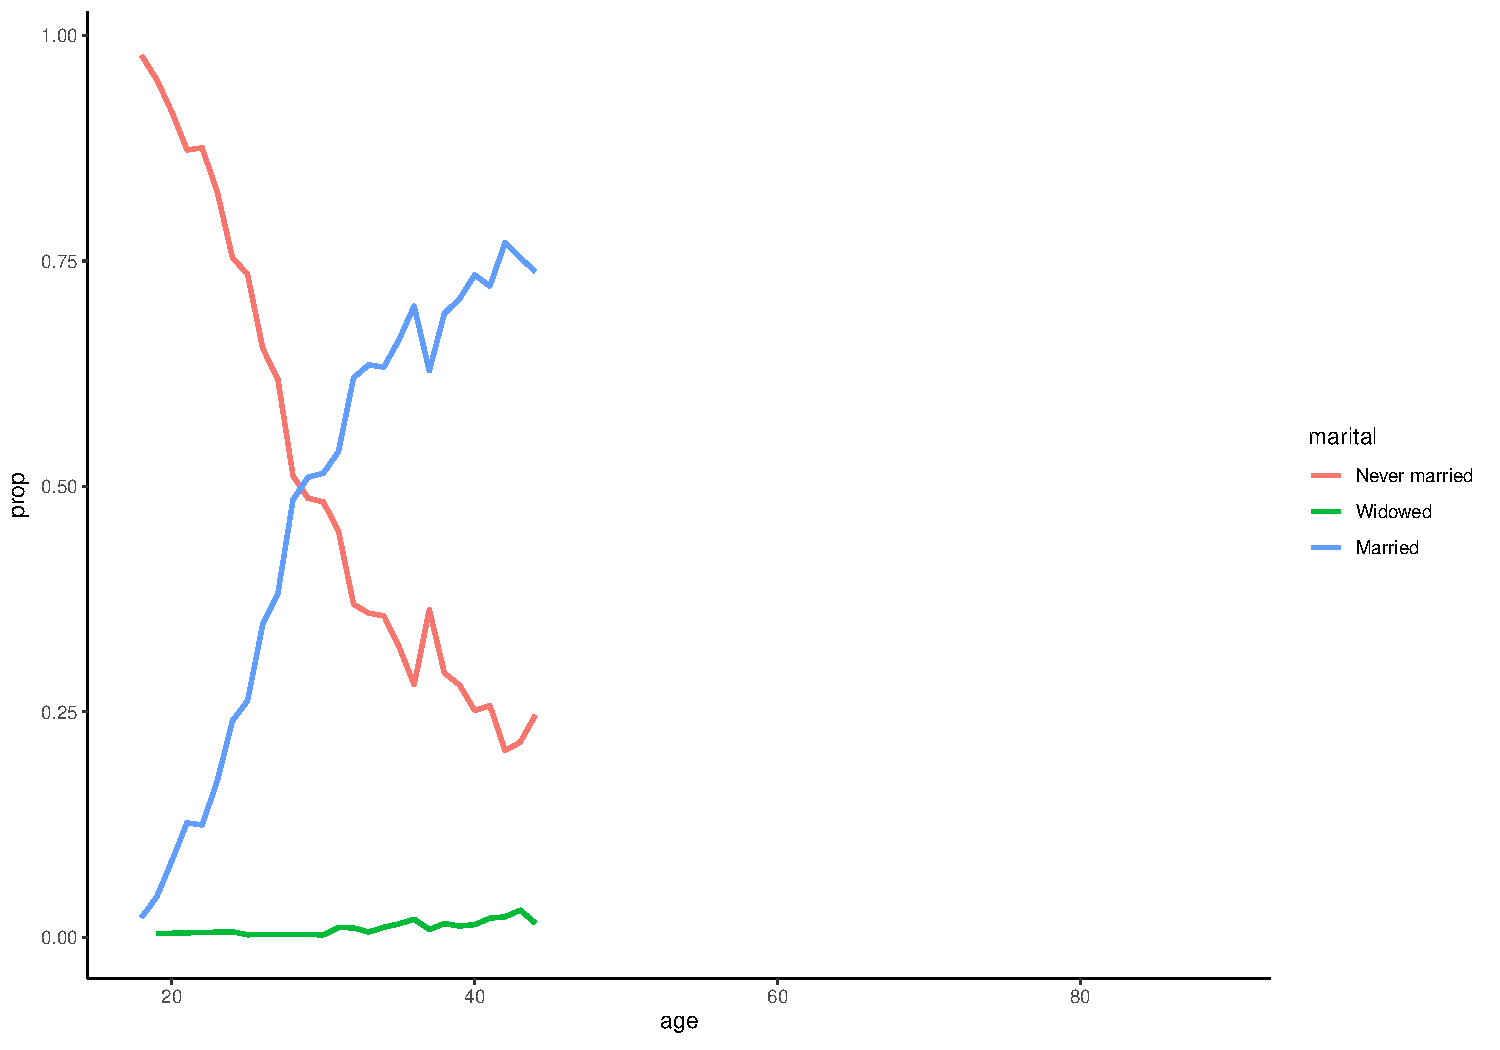
\includegraphics{gss_cat_files/figure-beamer/unnamed-chunk-1-41.pdf}

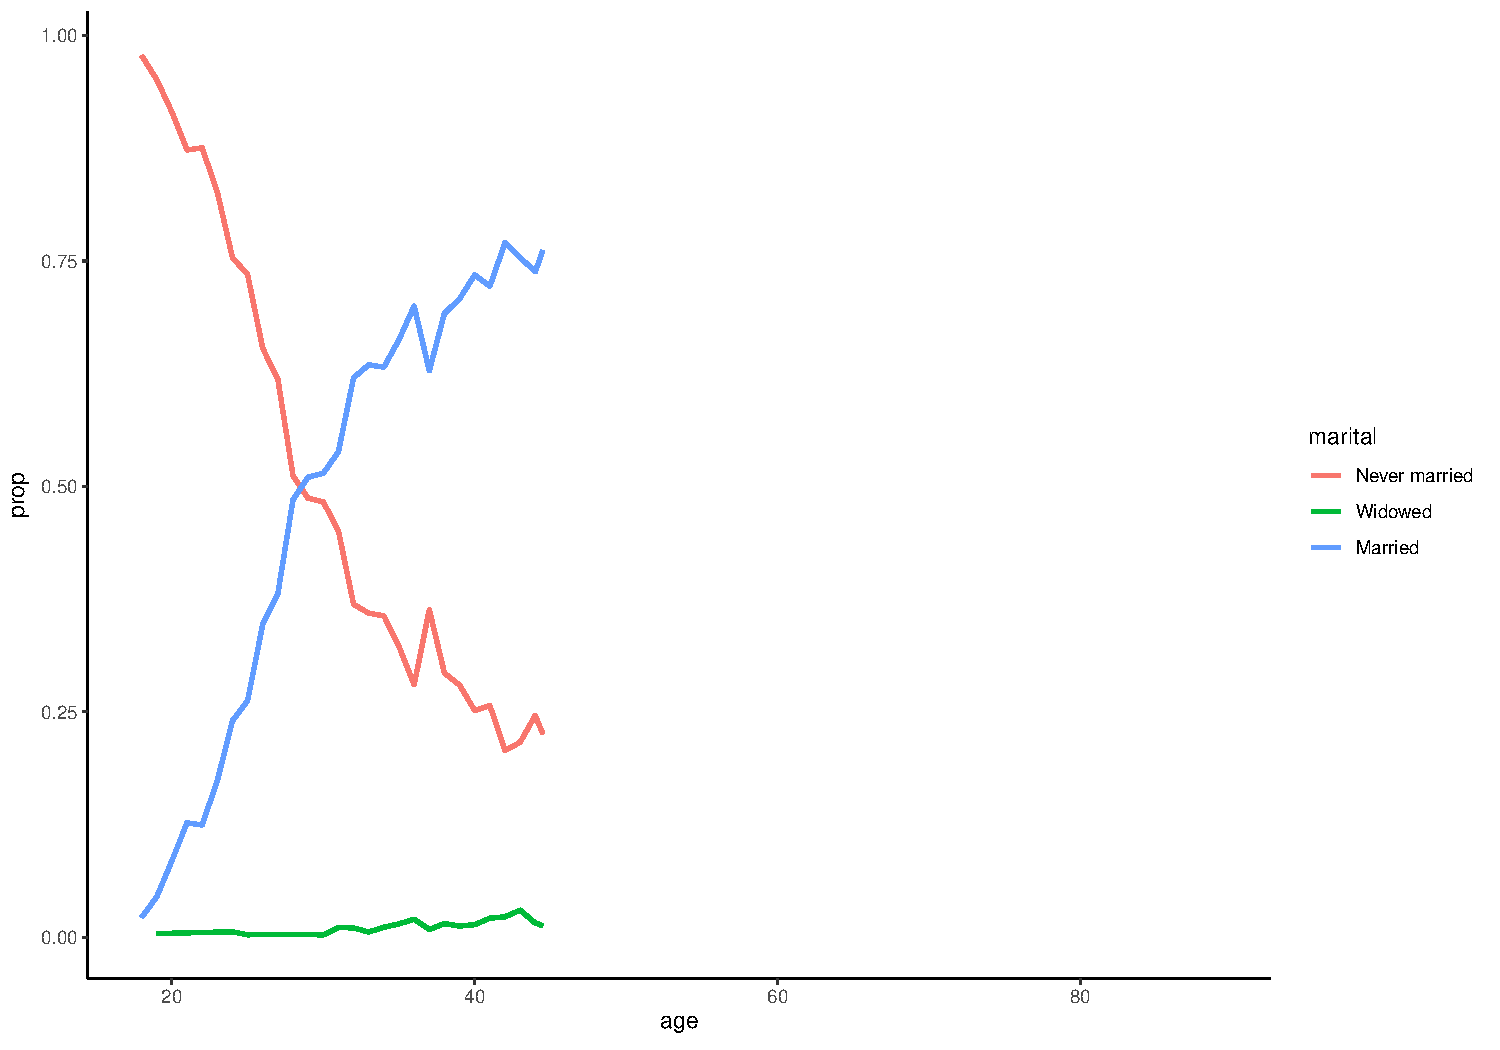
\includegraphics{gss_cat_files/figure-beamer/unnamed-chunk-1-42.pdf}

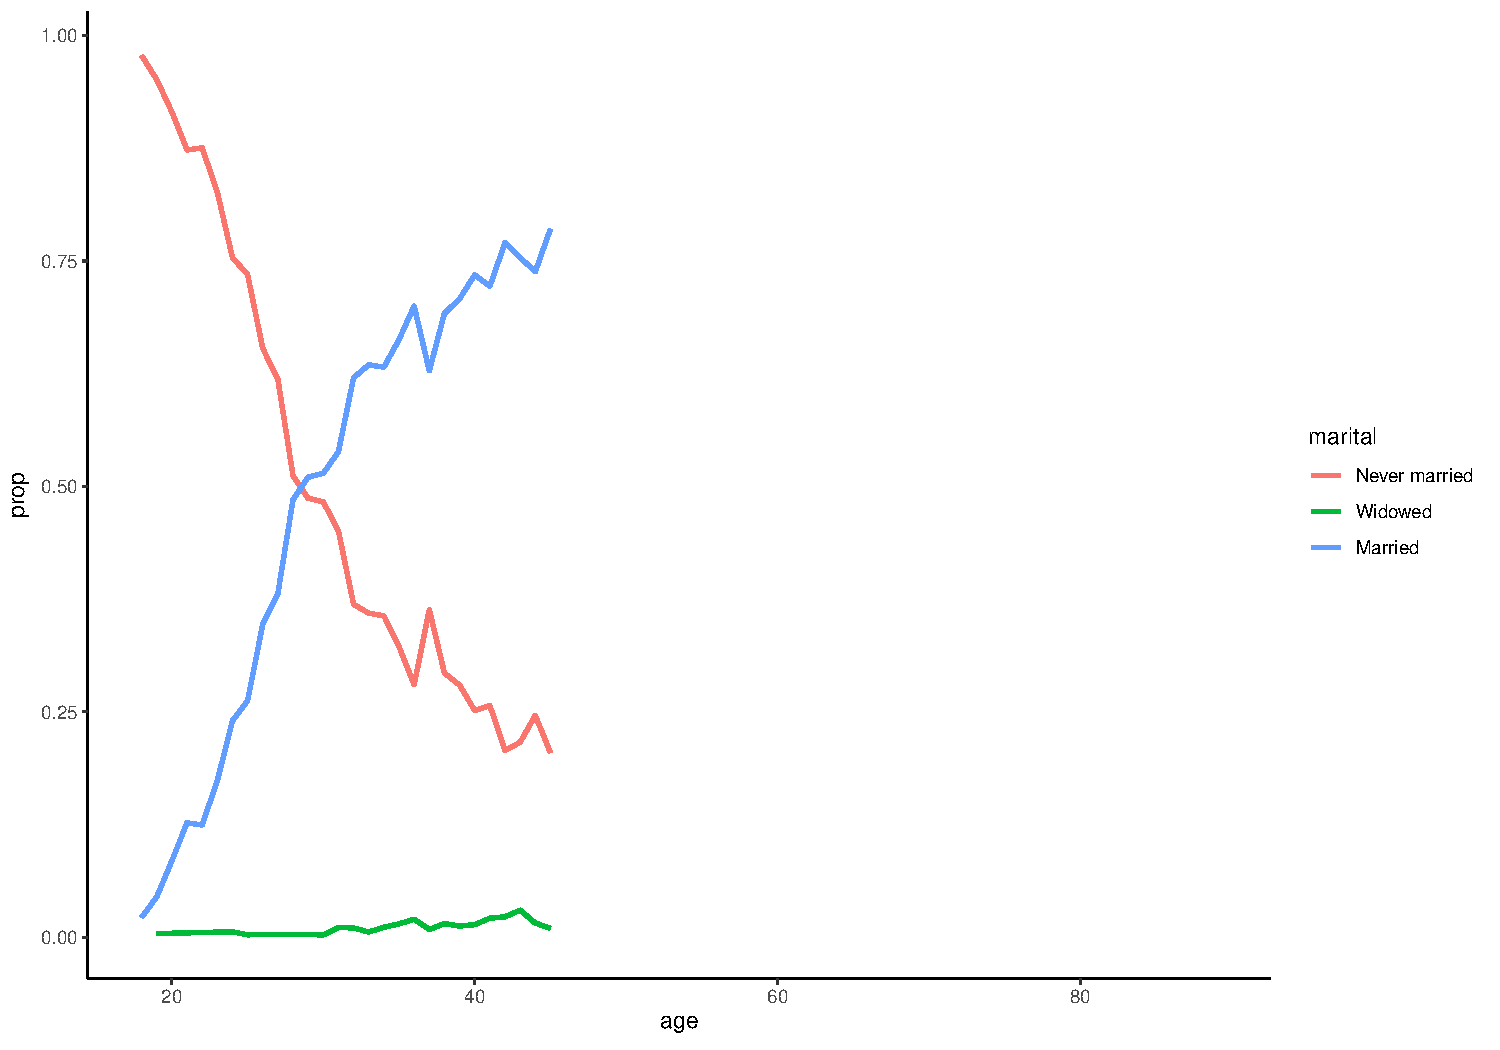
\includegraphics{gss_cat_files/figure-beamer/unnamed-chunk-1-43.pdf}

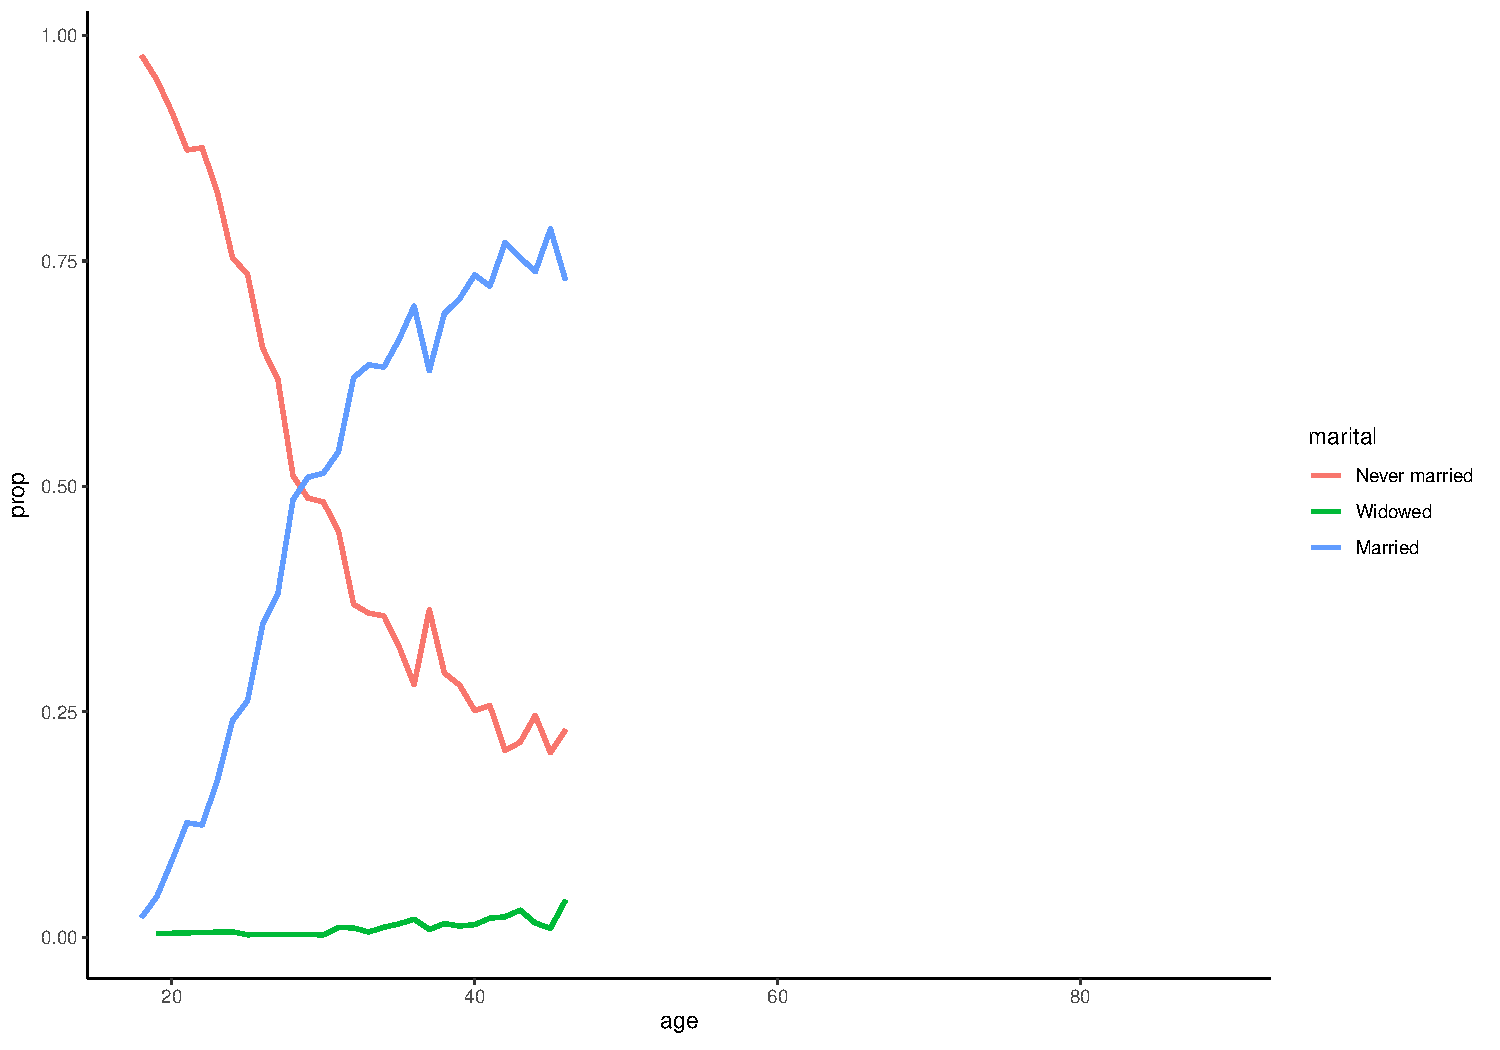
\includegraphics{gss_cat_files/figure-beamer/unnamed-chunk-1-44.pdf}

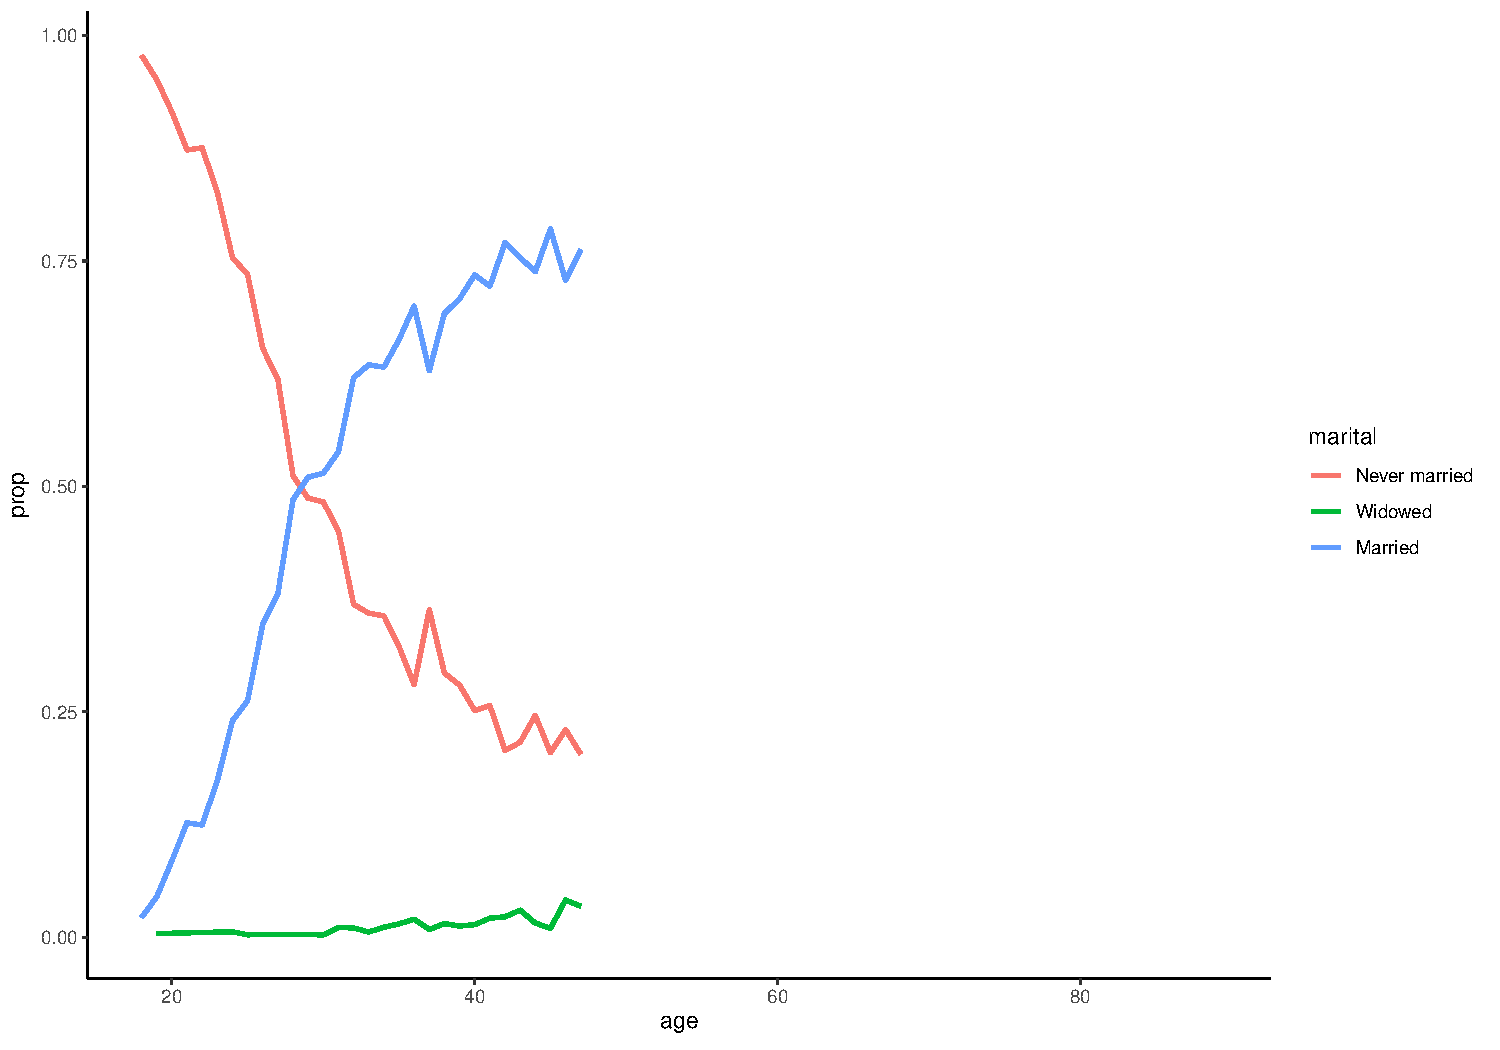
\includegraphics{gss_cat_files/figure-beamer/unnamed-chunk-1-45.pdf}

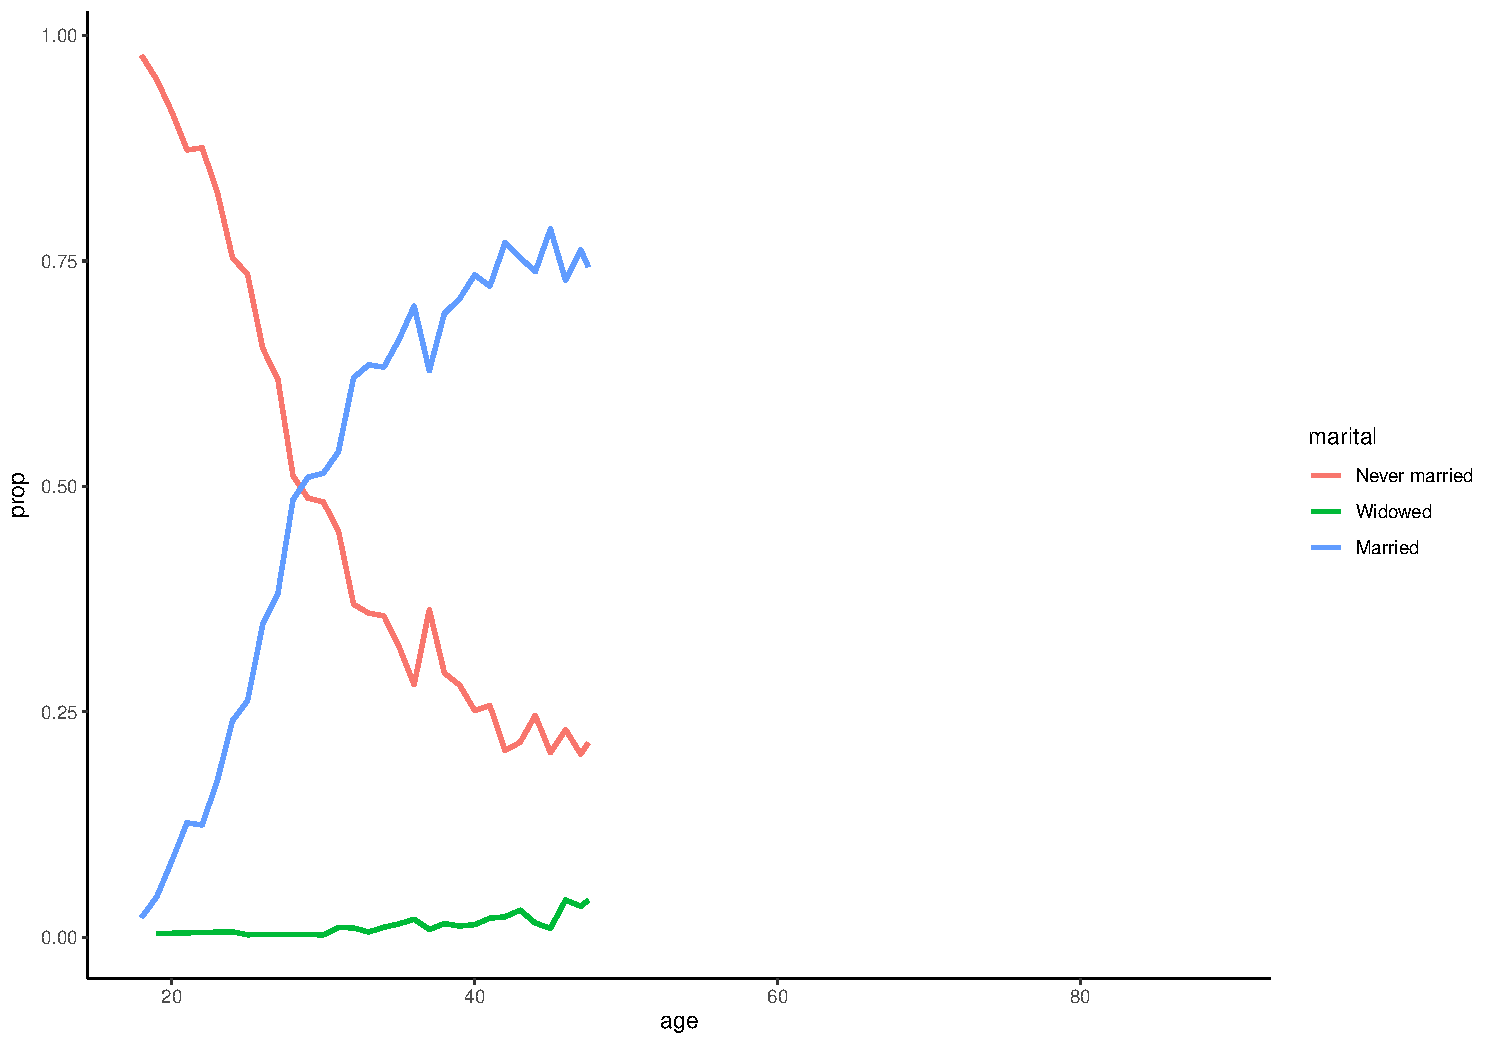
\includegraphics{gss_cat_files/figure-beamer/unnamed-chunk-1-46.pdf}

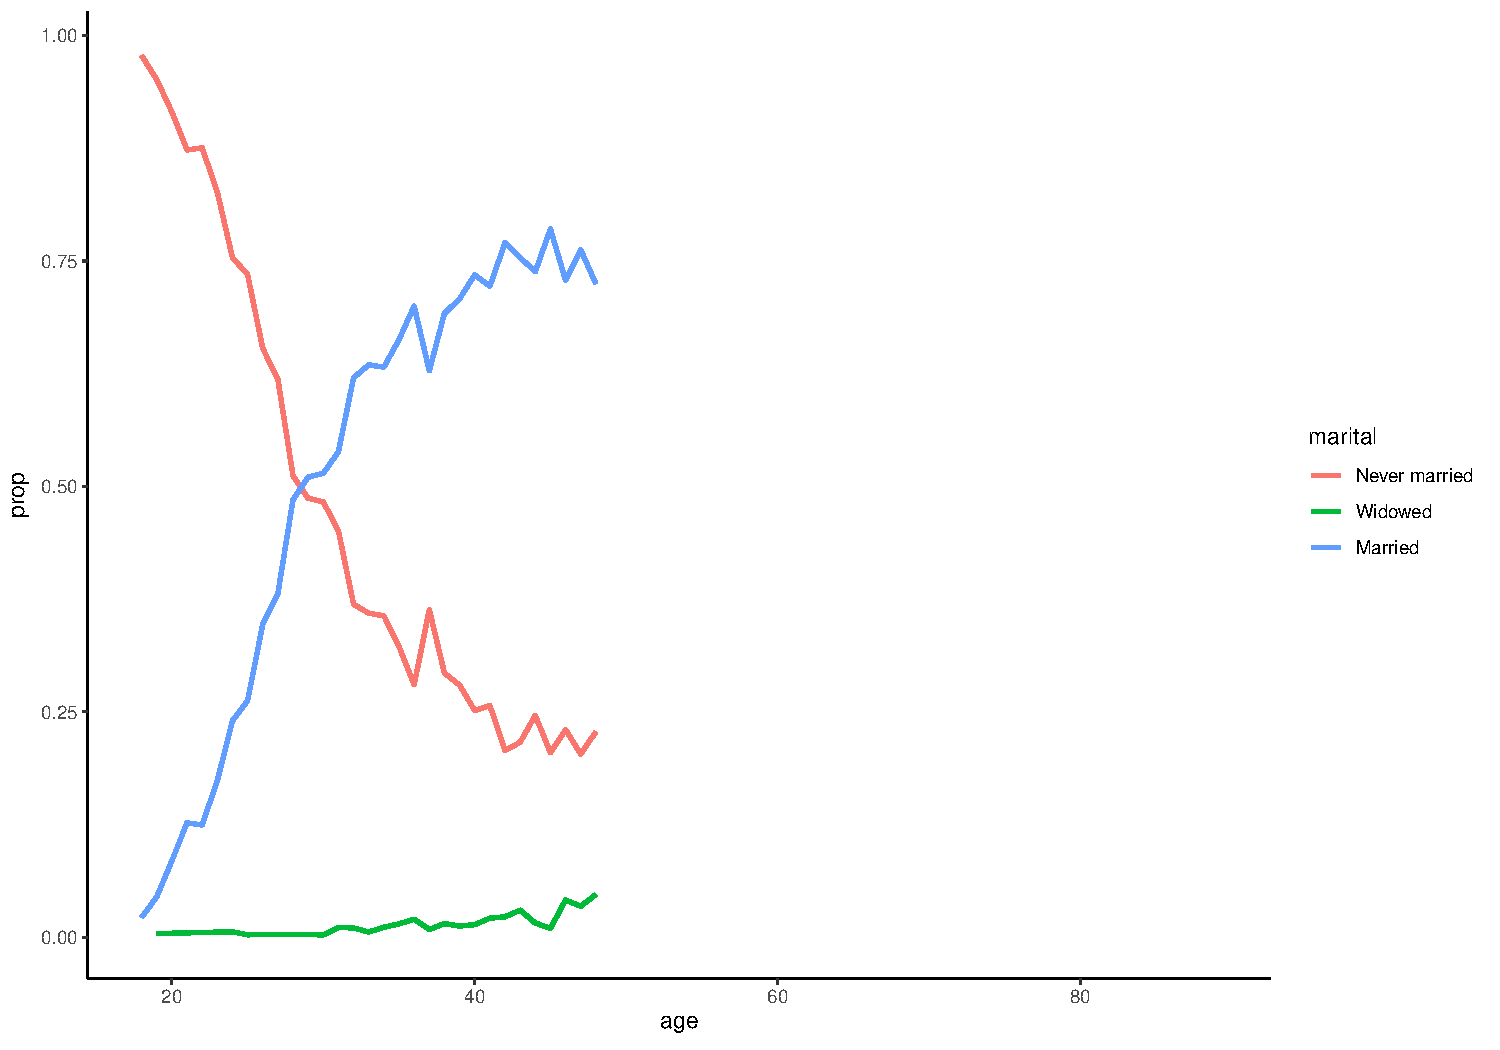
\includegraphics{gss_cat_files/figure-beamer/unnamed-chunk-1-47.pdf}

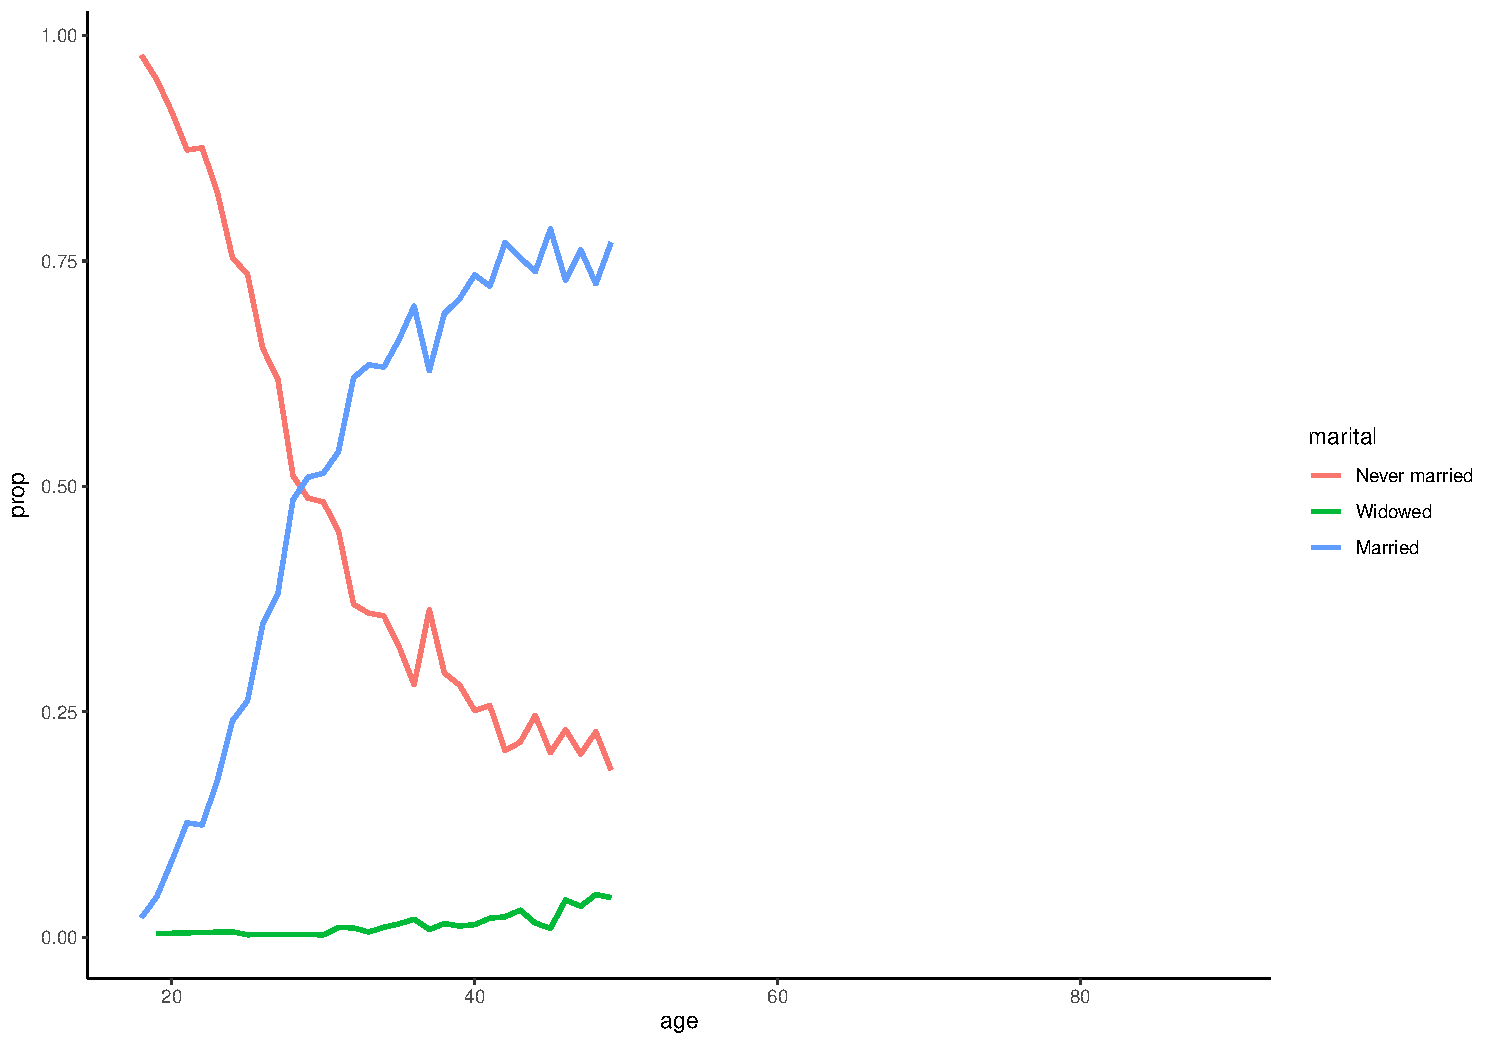
\includegraphics{gss_cat_files/figure-beamer/unnamed-chunk-1-48.pdf}

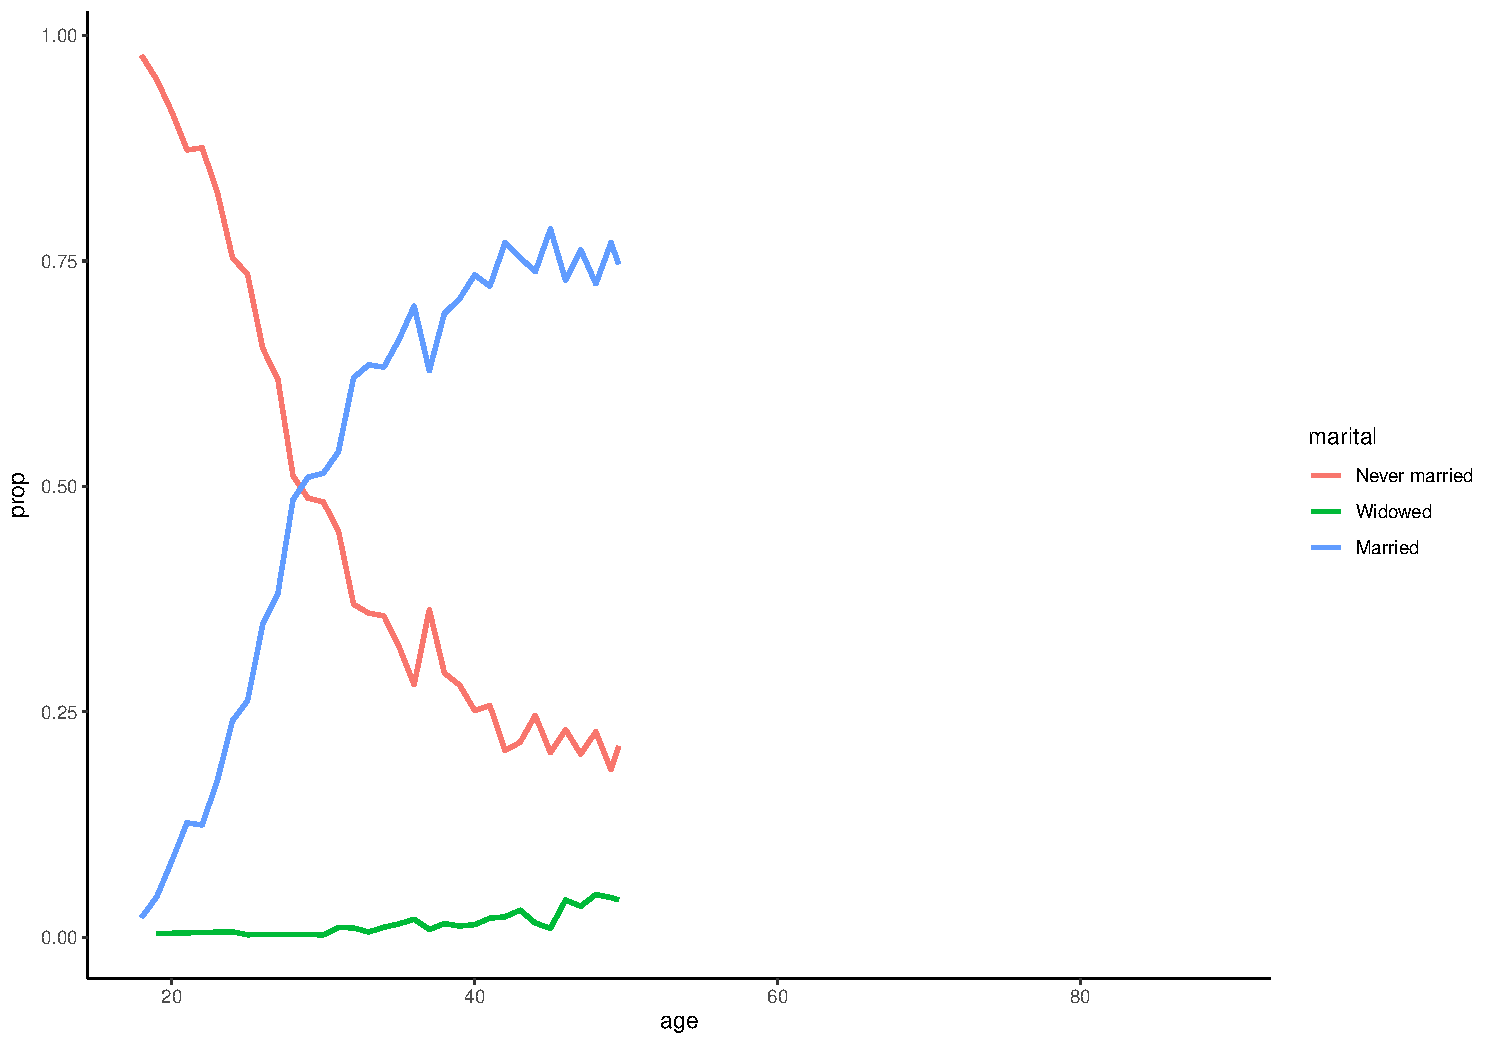
\includegraphics{gss_cat_files/figure-beamer/unnamed-chunk-1-49.pdf}

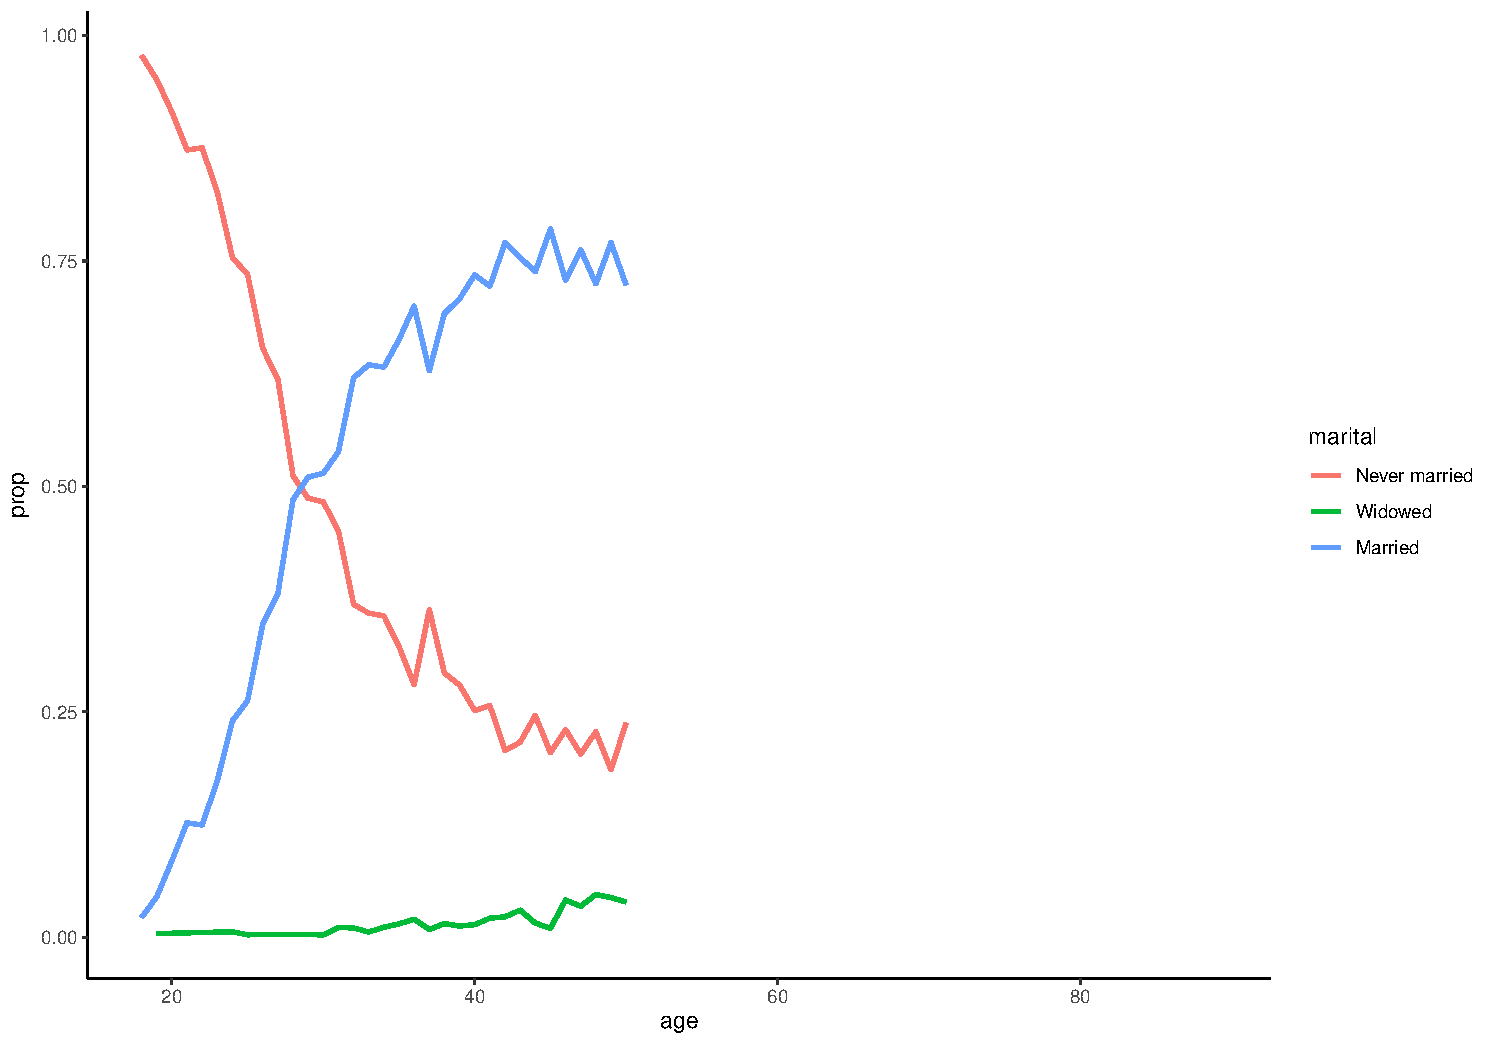
\includegraphics{gss_cat_files/figure-beamer/unnamed-chunk-1-50.pdf}

\includegraphics{gss_cat_files/figure-beamer/unnamed-chunk-1-51.pdf}

\includegraphics{gss_cat_files/figure-beamer/unnamed-chunk-1-52.pdf}

\includegraphics{gss_cat_files/figure-beamer/unnamed-chunk-1-53.pdf}

\includegraphics{gss_cat_files/figure-beamer/unnamed-chunk-1-54.pdf}

\includegraphics{gss_cat_files/figure-beamer/unnamed-chunk-1-55.pdf}

\includegraphics{gss_cat_files/figure-beamer/unnamed-chunk-1-56.pdf}

\includegraphics{gss_cat_files/figure-beamer/unnamed-chunk-1-57.pdf}

\includegraphics{gss_cat_files/figure-beamer/unnamed-chunk-1-58.pdf}

\includegraphics{gss_cat_files/figure-beamer/unnamed-chunk-1-59.pdf}

\includegraphics{gss_cat_files/figure-beamer/unnamed-chunk-1-60.pdf}

\includegraphics{gss_cat_files/figure-beamer/unnamed-chunk-1-61.pdf}

\includegraphics{gss_cat_files/figure-beamer/unnamed-chunk-1-62.pdf}

\includegraphics{gss_cat_files/figure-beamer/unnamed-chunk-1-63.pdf}

\includegraphics{gss_cat_files/figure-beamer/unnamed-chunk-1-64.pdf}

\includegraphics{gss_cat_files/figure-beamer/unnamed-chunk-1-65.pdf}

\includegraphics{gss_cat_files/figure-beamer/unnamed-chunk-1-66.pdf}

\includegraphics{gss_cat_files/figure-beamer/unnamed-chunk-1-67.pdf}

\includegraphics{gss_cat_files/figure-beamer/unnamed-chunk-1-68.pdf}

\includegraphics{gss_cat_files/figure-beamer/unnamed-chunk-1-69.pdf}

\includegraphics{gss_cat_files/figure-beamer/unnamed-chunk-1-70.pdf}

\includegraphics{gss_cat_files/figure-beamer/unnamed-chunk-1-71.pdf}

\includegraphics{gss_cat_files/figure-beamer/unnamed-chunk-1-72.pdf}

\includegraphics{gss_cat_files/figure-beamer/unnamed-chunk-1-73.pdf}

\includegraphics{gss_cat_files/figure-beamer/unnamed-chunk-1-74.pdf}

\includegraphics{gss_cat_files/figure-beamer/unnamed-chunk-1-75.pdf}

\includegraphics{gss_cat_files/figure-beamer/unnamed-chunk-1-76.pdf}

\includegraphics{gss_cat_files/figure-beamer/unnamed-chunk-1-77.pdf}

\includegraphics{gss_cat_files/figure-beamer/unnamed-chunk-1-78.pdf}

\includegraphics{gss_cat_files/figure-beamer/unnamed-chunk-1-79.pdf}

\includegraphics{gss_cat_files/figure-beamer/unnamed-chunk-1-80.pdf}

\includegraphics{gss_cat_files/figure-beamer/unnamed-chunk-1-81.pdf}

\includegraphics{gss_cat_files/figure-beamer/unnamed-chunk-1-82.pdf}

\includegraphics{gss_cat_files/figure-beamer/unnamed-chunk-1-83.pdf}

\includegraphics{gss_cat_files/figure-beamer/unnamed-chunk-1-84.pdf}

\includegraphics{gss_cat_files/figure-beamer/unnamed-chunk-1-85.pdf}

\includegraphics{gss_cat_files/figure-beamer/unnamed-chunk-1-86.pdf}

\includegraphics{gss_cat_files/figure-beamer/unnamed-chunk-1-87.pdf}

\includegraphics{gss_cat_files/figure-beamer/unnamed-chunk-1-88.pdf}

\includegraphics{gss_cat_files/figure-beamer/unnamed-chunk-1-89.pdf}

\includegraphics{gss_cat_files/figure-beamer/unnamed-chunk-1-90.pdf}

\includegraphics{gss_cat_files/figure-beamer/unnamed-chunk-1-91.pdf}

\includegraphics{gss_cat_files/figure-beamer/unnamed-chunk-1-92.pdf}

\includegraphics{gss_cat_files/figure-beamer/unnamed-chunk-1-93.pdf}

\includegraphics{gss_cat_files/figure-beamer/unnamed-chunk-1-94.pdf}

\includegraphics{gss_cat_files/figure-beamer/unnamed-chunk-1-95.pdf}

\includegraphics{gss_cat_files/figure-beamer/unnamed-chunk-1-96.pdf}

\includegraphics{gss_cat_files/figure-beamer/unnamed-chunk-1-97.pdf}

\includegraphics{gss_cat_files/figure-beamer/unnamed-chunk-1-98.pdf}

\includegraphics{gss_cat_files/figure-beamer/unnamed-chunk-1-99.pdf}

\includegraphics{gss_cat_files/figure-beamer/unnamed-chunk-1-100.pdf}

\includegraphics{gss_cat_files/figure-beamer/unnamed-chunk-1-101.pdf}

\includegraphics{gss_cat_files/figure-beamer/unnamed-chunk-1-102.pdf}

\includegraphics{gss_cat_files/figure-beamer/unnamed-chunk-1-103.pdf}

\includegraphics{gss_cat_files/figure-beamer/unnamed-chunk-1-104.pdf}
\end{frame}




\end{document}
